\documentclass[a4paper, 11pt]{article}

\usepackage[version=3]{mhchem}
\usepackage{siunitx}
\usepackage{graphicx}
\usepackage{amsmath}
\usepackage[total={16cm,25cm}, top=3cm, left=2.5cm, includefoot]{geometry}
\usepackage{pgfplots}
\usepackage{float}
\usepackage{amsfonts}
\usepackage{booktabs}
\usepackage{easytable}
\usepackage{mathtools}
\usepackage{comment}
\usepackage[makeroom]{cancel}
\renewcommand{\figurename}{Obrázek}
\renewcommand{\refname}{Zdroje}
\renewcommand{\tablename}{Tabulka}
\renewcommand{\contentsname}{Obsah}

\setlength\parindent{0pt}
\setcounter{section}{0}
\renewcommand{\labelenumi}{\alph{enumi}.}
\usepackage{xcolor}
\definecolor{light-gray}{gray}{0.95}
\newcommand{\code}[1]{\colorbox{light-gray}{\texttt{#1}}}
\newcommand{\logoCVUT}{
\includegraphics[width = 0.5\textwidth]{img/symbol_cvut_konturova_verze_cb.pdf}}
\newcommand{\logoFJFI}{
\includegraphics[width = 0.4\textwidth]{img/fjfi_logo.png}}

\begin{document}
% \section*{Seznam použitých veličin}
\addcontentsline{toc}{section}{Seznam použitých veličin}
\markboth{Seznam použitých veličin}{Seznam použitých veličin}

\renewcommand{\arraystretch}{1.2}
\begin{table}[H]
\begin{tabular}{p{1cm}l}
  $B_g$           & geometrický faktor (1/cm) \\
  $B_m$           & materiálový faktor (1/cm) \\
  $B_n$           & vlastní číslo (1/cm) \\
  $D$             & difúzní koeficient (cm) \\
  $\Phi$          & hustota toku neutronů (1/cm$^2$s) \\
  $k_{\text{ef}}$ & koeficient násobení (-) \\
  $k_{\infty}$    & koeficient násobení pro nekonečný systém (-) \\
  $\ell$          & střední doba života neutronů (s) \\
  $L$             & difúzní délka (cm) \\
  $L^2$           & difúzní plocha (cm$^2$) \\
  $\Lambda$       & střední doba vzniku neutronů (s) \\
  $n$             & hustota neutronů (1/cm$^3$) \\
  $N$             & počet neutronů (-) \\
  $P$             & výkon (tepelný) (W) \\
  $\Psi_n$        & vlastní funkce (-) \\
  $Q$             & zdroj neutronů (1/cm$^3$s) \\
  $\textbf{r}$    & polohový vektor (cm) \\
  $\rho$          & reaktivita (-) \\
  $\Sigma$        & makroskopický účinný průřez (1/cm) \\
  $\Sigma_a$      & makroskopický účinný průřez pro absorbci (1/cm) \\
  $\Sigma_f$      & makroskopický účinný průřez pro štěpení (1/cm) \\
  $t$             & čas (s) \\
  $T_e$           & perioda reaktoru (s) \\
  $v$             & rychlost (m/s) \\

\end{tabular}
\end{table}
\renewcommand{\arraystretch}{1}

% \section*{Seznam použitých zkratek}
\addcontentsline{toc}{section}{Seznam použitých zkratek}
\markboth{Seznam použitých zkratek}{Seznam použitých zkratek}

\renewcommand{\arraystretch}{1.2}
\begin{table}[H]
\begin{tabular}{p{1cm}l}
  AZ           & aktivní zóna \\
  1G           & 1-grupová \\
  2G           & 2-grupová \\
  FR           & rychlý reaktor -- Fast Reactor \\
  LS           & levá strana \\
  LT           & Laplaceova transformace \\
  LWR          & lehkovodní reaktor -- Light Water Reactor \\
  PS           & pravá strana \\
  ZV           & zpětná vazba \\
\end{tabular}
\end{table}
\renewcommand{\arraystretch}{1}


% titulní strana
\thispagestyle{empty}

\begin{center}
	{\LARGE
		České vysoké učení technické v Praze \par
		Fakulta jaderná a fyzikálně inženýrská
	}
    \vspace{10mm}

    \begin{tabular}{c}
		\textbf{Katedra jaderných reaktorů} \\[3pt]
    \end{tabular}

   \vspace{10mm} \logoCVUT \vspace{15mm}

   {\huge \textbf{Fyzika jaderných reaktorů}\par}
   \vspace{5mm}
   {\huge \textbf{Magisterské studium}\par}

   \vspace{15mm}
   {\Large \MakeUppercase{Státnicové otázky}}

   \vfill
   {\large
    \begin{tabular}{ll}
    Rok: & 2025
    \end{tabular}
   }
\end{center}

% Prohlášení
\newpage
\thispagestyle{empty}

%~
\vfill

\vspace{1em}
Čau ahoj. Právě čtete soubor magisterských státnicových otázek k předmětu Fyzika jaderných reaktorů, který byl vypracován za dlouhých zimních večerů v pokojíku ve Švýcarsku. Jedná se o sepis všech prezentací, skript a materiálů, ze kterých jsme během výuky čerpali, a které jsou dle mého názoru k pochopění nejdůležitější. Šlo zejména o:

\begin{itemize}
    \item prezentace k předmětu ZAF (J. Frýbort, L. Frýbortová, M. Štefánik),
    \item prezentace k předmětu FARE (J. Frýbort),
    \item prezentace k předmětu DERF (J. Frýbort a P. Suk),
    \item přednášky z předmětu SMRF (O. Huml),
    \item přednášky z předmětu KID (O. Huml),
    \item zápisky z předmětu KID (O. Huml),
    \item Dynamika jaderných reaktorů -- B. Heřmanský,
    \item Nuclear Reactor Physics -- W. Stacey,
    \item Introduction to Nuclear Engineering -- J. Lamarsch,
    \item Development of a New Monte Carlo Reactor Physics Code -- J. Leppänen,
    \item Numerical Methods for Nuclear Fuel Burnup Calculations -- M. Pusa,
    \item manuál ke kódu NJOY,
    \item manuál ke kódu SCALE,
    \item manuál ke kódu MCNP,
    \item manuál ke kódu Serpent,
    \item prezentace MCNP z LANL,
    \item a spoustu dalšího.
\end{itemize}

Pokud najdete chybu, hoďte issue na Git: \it{https://github.com/saboljos/FJR\_statnicove-otazky}.\\

\rm Hodně zdaru!

\rm J.S.

\vspace{2em}

\clearpage{\pagestyle{empty}}

\include{none}

\newpage
\parskip=0pt
\begin{small}
\tableofcontents
\end{small}
\parskip=7pt
\newpage

\section[Difúzní teorie]{Odvození a využití difuzní teorie v reaktorové fyzice}
\section[Metody jader a vlastních funkcí]{Zavedení metody jader a metody vlastních funkcí pro řešení úloh z reaktorové fyziky a transportu záření}
\section[Transportní rovnice]{Odvození a využití transportní teorie v reaktorové fyzice}

Transportní rovnice je základní matematický model používaný v reaktorové fyzice k popisu pohybu a interakce neutronů v materiálu. Její cílem je určit rozložení neutronů v prostoru, energii a čase v jaderném reaktoru nebo jiném prostředí.

Momentálně se jedná o rovnici, která co nejvěrněji popisuje chování a šíření neutronů, nicméně její zápis je příliš složitý a neexistuje obecné analytické řešení. Z toho důvodu je nutné přecháet k určitým zjednodušením, kterými může být například difúzní rovnice.

\subsection{Boltzmanova integro-diferenciální transportní rovnice}

Odvození musí nutně vycházet z dějů, které má popisovat. Vzhledem k běžným podmínkám v reaktorech je možné popis chování neutronů zúžit na úlohu neutrálních částic pohybujících se podle zákonitostí klasické mechaniky s kvantovým popisem jejich interakcí s jádry okolního prostředí.

Cílem je převést izolovanou částicovou povahu interakcí neutronů na spojitou veličinu.

\subsubsection{Předpoklady}

Pro odvození musíme předpokládat:

\begin{itemize}
  \item dostatečná populace neutronů, abychom mohli uvažovat statistické středování,
  \item neutrony interagují pouze s jádry okolí (která jsou v klidu) a nikoliv mezi sebou $\rightarrow$ v reaktorech splněno vždy (projevuje se až pro $\Phi > 10^{20}$ 1/cm$^2$/s).
\end{itemize}

\subsubsection{Matematický aparát}

Pro odvození je potřeba zavést:

\textbf{a) Nezávislé proměnné}:

Nezávislé proměnné představují souřadnice, pomocí kterých jsme schopni neutronům přiřadit bod fázového prostoru. Pro jednoznačné určení je potřeba 6~nezávislých proměnných (v klasické mechanice jde o 3~složky polohového vektoru a 3~složky vektoru rychlosti), nicméně v tomto případě se od vektoru rychlosti přechází ke směru pohybu a velikosti rychlosti.

Pro popis tedy předpokládáme:

\begin{itemize}
  \item polohový vektor $\textbf{r} = (x, y, z)$ -- 3 složky,
  \item směrový vektor $\Omega = (\phi, \theta)$ -- 2 složky,
  \item (kinetická) energie $E$ -- 1 složka.
\end{itemize}

Pro případný přepočet poté platí:

$$ v = \sqrt{\dfrac{2m}{E}}, $$
$$ \textbf{v} = v \Omega. $$

Časovou závislost zanedbáváme a na čas nahlížíme jako na parametr, nikoliv souřadnici.

\textbf{b) Fázový prostor:}

Představuje prostor pro popis neutronových interakcí. Základním předpokladem je zachování částicové povahy neutronů při využití statistické povahy pohybu velkého množství částic. Jednotlivé srážky se proto odehrávají ve statisticky středovaném \textbf{elementu fázového prostoru} $\Delta \textbf{P}$:

$$ \Delta \textbf{P} = \Delta \textbf{r} \Delta \Omega \Delta \textbf{E}. $$

Počet neutronů v $\Delta \textbf{P}$ se může změnit vlivem změny v dílčích parametrech, tedy:

\begin{itemize}
  \item v $\Delta \textbf{r}$ -- únikem z $\Delta \textbf{r}$, případně absorbcí nebo vznikem v $\Delta \textbf{r}$,
  \item v $\Delta \Omega$ -- rozptylem,
  \item v $\Delta E$ -- zpomalením, nebo zrychlením.
\end{itemize}

\textbf{c) Závislé proměnné:}

Dále je potřeba zavést závislé proměnné (závislé od toho, že jsou závislé na těch nezávislých a času), které představují sledované veličiny.

Sem řadíme 3 základní:

\begin{itemize}
  \item úhlová hustota neutronů $n(\textbf{r}, \Omega, E, t)$ (1/cm$^3$) -- skalár,
  \item úhlová hustota toku neutronů $\Omega(\textbf{r}, \Omega, E, t)$ (1/cm$^2$/s) -- skalár (ale bacha, neplést se směrovým vektorem $\Omega$),
  \item úhlová hustota proudu neutronů $\textbf{J}(\textbf{r}, \Omega, E, t)$ (1/cm$^2$/s) -- vektor
\end{itemize}

s definovanými vztahy:

\begin{equation}
  \boxed{
  \Phi(\textbf{r}, \Omega, E, t) = v \cdot n(\textbf{r}, \Omega, E, t),
  \label{definice_hustota_toku}}
\end{equation}

\begin{equation}
  \boxed{
  \textbf{J}(\textbf{r}, \Omega, E, t) = \Omega \cdot \Phi(\textbf{r}, \Omega, E, t).
  \label{definice_hustota_proudu}}
\end{equation}

Pro kontext, \textbf{$\Phi$ udává celkový součet drah všech neutronů za sekundu v jednotkovém objemu fázového prostoru}, zatímco \textbf{$\textbf{J}$ udává počet neutronů, který prochází na steradián, energii a plochu ve směru $\Omega$ plochou kolmou k $\Omega$ v čase}. Tedy, zatímco $n$ a $\Phi$ se vztahují k objemu, $\textbf{J}$ se vztahuje k ploše.

\subsubsection{Odvození}

Nejprve je potřeba si uvědomit, jak popisujeme interakce neutronů s jádry. Pravděpodobnost interakce je dána $\sigma$ (cm$^2$) a $\Sigma$ (1/cm), přičemž mezi možné interakce řadíme pouze: rozptyl, radiační záchyt a štěpení, případně absorbci (což je součet štěpení a radiačního záchytu).

\textbf{Makroskopický účinný průřez pro interakci $i$ na jádře $j$} -- $\Sigma_{ij}(\textbf{r}, E, t)$ definujeme jako podíl pravděpodobnosti interakce neutronu reakcí $i$ s jádrem $j$ na jednotku délky dráhy.

Dále \textbf{reakční rychlost pro interakci $i$ na jádře $j$} -- $F_{ij}(\textbf{r}, E, t)$ určíme jako:

$$ F_{ij}(\textbf{r}, E, t) = \Sigma_{ij}(\textbf{r}, E, t) \Phi(\textbf{r}, E, t). $$

Při předpokladu nezávislosti jednotlivých interakcí (abychom mohli průřezy sčítat) je možné definovat totální makroskopický účinný průřez:

$$ \Sigma_i(\textbf{r}, E, t) = \sum_{j=1}^J \Sigma_{ij}(\textbf{r}, E, t) = \sum_{j=1}^J N_j(\textbf{r}, t) \sigma_{ij}(E). $$

Dále si pro popis rozptylu zavedeme \textbf{diferenciální rozptylové jádro} -- $f_s(\Omega' \cdot \Omega, E' \rightarrow E)$ (-) tak, že:

\begin{itemize}
  \item $f_s(\Omega' \cdot \Omega, E' \rightarrow E) \Delta \Omega \Delta E$ značí poměrnou pravděpodobnost rozptylu ze směru $\Omega'$ a energie $E'$ do rozsahu směrů $\Delta \Omega$ a energií $\Delta E$,
  \item pro rozptyl na jádře $j$ platí:
\end{itemize}
$$\Sigma_{sj}(\textbf{r}, \Omega' \cdot \Omega, E' \rightarrow E, t) = \Sigma_{sj}(\textbf{r}, E', t) f_s(\Omega' \cdot \Omega, E' \rightarrow E), $$

\begin{itemize}
  \item pro účely normalizace platí:
\end{itemize}
$$\int_\mathbb{R^+} \int_{4 \pi} f_s(\Omega' \cdot \Omega, E' \rightarrow E) \text{d} \Omega \text{d}E = 1. $$


Pro odvození musíme vycházet z bilanční rovnice neutronů, kde sledujeme změnu počtu neutronů v libovolném elementu fázového prostoru tvořeném objemem $V$ a $\Delta \Omega \Delta E$ během časového intervalu $\Delta t$.

Jednodušeji řečeno posuzujeme jednotlivé příspěky či ztráty neutronů:

\begin{equation}
  \boxed{
  \begin{pmatrix} \text{počet neutronů} \\ \text{v čase } t + \Delta t \end{pmatrix} = \begin{pmatrix} \text{počet neutronů} \\ \text{v čase } t \end{pmatrix} + \begin{pmatrix} \text{zisk neutronů} \\ \text{během } \Delta t \end{pmatrix} - \begin{pmatrix} \text{ztráta neutronů} \\ \text{během } \Delta t \end{pmatrix}.
  \label{bilancni_rovnice}}
\end{equation}

Nyní popíšeme jednotlivé stavy:

\textbf{a) Počet neutronů v čase $t + \Delta t$:}

$$ \Delta \Omega \Delta E \int_V n(\textbf{r}, \Omega, E, t + \Delta t) \text{d}V $$

\textbf{b) Počet neutronů v čase $t$:}

$$ \Delta \Omega \Delta E \int_V n(\textbf{r}, \Omega, E, t) \text{d}V $$

\textbf{c) Zisk neutronů během $\Delta t$:}

Zisk neutronů se skládá ze zisku:

\begin{itemize}
  \item rozptylem:
\end{itemize}
$$ \Delta \Omega \Delta E \Delta t \int_V \int_\mathbb{R^+} \int_{4 \pi} f_s(\Omega' \cdot \Omega, E' \rightarrow E) \Sigma_s(\textbf{r}, E', t) \Phi(\textbf{r}, \Omega', E', t) \text{d}\Omega' \text{d}E' \text{d}V, $$

\begin{itemize}
  \item štěpením:
\end{itemize}
$$ \Delta \Omega \Delta E \Delta t \dfrac{\chi(E)}{4 \pi} \int_V \int_\mathbb{R^+} \int_{4 \pi} \nu(E') \Sigma_f(\textbf{r}, E', t) \Phi(\textbf{r}, \Omega', E', t) \text{d}\Omega' \text{d}E' \text{d}V. $$


Štěpení se předpokládá izotropní (skutečně je) a neuvažují se zpožděné neutrony. Pro distribuční funkci $\chi(E)$ musí platit:

$$ \int_\mathbb{R^+} \chi(E) \text{d} E = 1. $$

\textbf{d) Ztráta neutronů během $\Delta t$:}

Ztráta neutronů se skládá ze ztráty:

\begin{itemize}
  \item rozptylem:
\end{itemize}
$$ \Delta \Omega \Delta E \Delta t \int_V \int_\mathbb{R^+} \int_{4 \pi} f_s(\Omega' \cdot \Omega, E \rightarrow E') \Sigma_s(\textbf{r}, E, t) \Phi(\textbf{r}, \Omega, E, t) \text{d}\Omega' \text{d}E' \text{d}V. $$

Veličiny $\Sigma_s$ a $\Phi$ nejsou závislé na čárkovaných veličinách (u zisku neutronů jsou, tam to provést nejde), takže je možné je z integrálu $\text{d}\Omega'$ a $\text{d}E'$ vytknout a využít normalizace rozptylového jádra (viz někde nahoře), čímž dostaneme:

$$ \Delta \Omega \Delta E \Delta t \int_V  \Sigma_s(\textbf{r}, E, t) \Phi(\textbf{r}, \Omega, E, t) \text{d}V, $$

\begin{itemize}
  \item absorbcí:
\end{itemize}
$$ \Delta \Omega \Delta E \Delta t \int_V  \Sigma_a(\textbf{r}, E, t) \Phi(\textbf{r}, \Omega, E, t) \text{d}V, $$

\begin{itemize}
  \item únikem:
\end{itemize}
$$ \Delta \Omega \Delta E \Delta t \oint_S  \textbf{J}(\textbf{r}, \Omega, E, t) \cdot \text{d}\textbf{S} = \Delta \Omega \Delta E \Delta t \int_V  \text{div} \textbf{J}(\textbf{r}, \Omega, E, t) \text{d}V.$$

Dohromady to vše dává nepřehlednou motanici:

\small
\begin{equation*}
\begin{multlined}
  \Delta \Omega \Delta E \int_V n(\textbf{r}, \Omega, E, t + \Delta t) \text{d}V = \Delta \Omega \Delta E \int_V n(\textbf{r}, \Omega, E, t) \text{d}V + \\
  + \Delta \Omega \Delta E \Delta t \int_V \int_\mathbb{R^+} \int_{4 \pi} f_s(\Omega' \cdot \Omega, E' \rightarrow E) \Sigma_s(\textbf{r}, E', t) \Phi(\textbf{r}, \Omega', E', t) \text{d}\Omega' \text{d}E' \text{d}V + \\
  + \Delta \Omega \Delta E \Delta t \dfrac{\chi(E)}{4 \pi} \int_V \int_\mathbb{R^+} \int_{4 \pi} \nu(E') \Sigma_f(\textbf{r}, E', t) \Phi(\textbf{r}, \Omega', E', t) \text{d}\Omega' \text{d}E' \text{d}V - \\ 
  - \Delta \Omega \Delta E \Delta t \int_V  \Sigma_s(\textbf{r}, E, t) \Phi(\textbf{r}, \Omega, E, t) \text{d}V - \Delta \Omega \Delta E \Delta t \int_V  \Sigma_a(\textbf{r}, E, t) \Phi(\textbf{r}, \Omega, E, t) \text{d}V - \\
  - \Delta \Omega \Delta E \Delta t \int_V  \text{div} \textbf{J}(\textbf{r}, \Omega, E, t) \text{d}V
\end{multlined}
\end{equation*}
\normalsize

Vykrátíme rovnici diferencemi $\Delta \Omega \Delta E \Delta t$, z definice nahradíme $n = \dfrac{\Phi}{v}$ a $\textbf{J} = \Omega \cdot \Phi$, uzavřeme do jednoho integrálu přes objem, výrazy přesuneme na jednu stranu a trochu přeskládáme:

\small
\begin{equation*}
\begin{multlined}
  \int_V \left [ \dfrac{1}{v} \left [ \dfrac{\Phi(\textbf{r}, \Omega, E, t + \Delta t) - (\textbf{r}, \Omega, E, t)}{\Delta t} \right ] + \left [ \Sigma_a + \Sigma_s \right ] \cdot \Phi(\textbf{r}, \Omega, E, t) + \text{div} \left [ \Omega(\textbf{r}, \Omega, E, t) \cdot \Phi(\textbf{r}, \Omega, E, t) \right ] \right ] \text{d}V - \\
  - \int_V \int_\mathbb{R^+} \int_{4 \pi} \left [ f_s(\Omega' \cdot \Omega, E' \rightarrow E) \Sigma_s(\textbf{r}, E', t) \Phi(\textbf{r}, \Omega', E', t) - \dfrac{\chi(E)}{4 \pi} \nu(E') \Sigma_f(\textbf{r}, E', t) \Phi(\textbf{r}, \Omega', E', t) \right ] \text{d}\Omega' \text{d}E' \text{d}V = 0.
\end{multlined}
\end{equation*}
\normalsize

Dále se limitně přejde z diferencí k diferenciálům, čímž se první zlomek s $\Phi$ změní v parciální derivaci. Součet průřezů dá: $\Sigma_s + \Sigma_a = \Sigma_t$, z rozepsání divergence přes indexy a aplikace derivace součinu vznikne: $\text{div} \left [ \Omega \cdot \Phi(\textbf{r}, \Omega, E, t) \right ] = \Omega \cdot \text{grad} \Phi(\textbf{r}, \Omega, E, t)$, součin rozptylového jádra s průřezem pro rozptyl dá: $f_s(\Omega' \cdot \Omega, E' \rightarrow E) \Sigma_s(\textbf{r}, E', t) = \Sigma_s(\textbf{r}, \Omega' \cdot \Omega, E' \rightarrow E, t)$ a zbavíme se integrálu přes objem, čímž lze dospět k tvaru:

\small
\begin{equation*}
\begin{multlined}
  \left [ \dfrac{1}{v} \dfrac{\partial}{\partial t} + \Sigma_t(\textbf{r}, E, t) + \Omega \cdot \text{grad} \right ]\Phi(\textbf{r}, \Omega, E, t) = \\
  = \int_\mathbb{R^+} \int_{4 \pi} \left [ \Sigma_s(\textbf{r}, \Omega' \cdot \Omega, E' \rightarrow E, t) + \dfrac{\chi(E)}{4 \pi} \nu(E') \Sigma_f(\textbf{r}, E', t)\right ] \Phi(\textbf{r}, \Omega', E', t) \text{d}\Omega' \text{d}E'.
\end{multlined}
\end{equation*}
\normalsize

Ještě se na pravou stranu přidá zdrojová podmínka $Q(\textbf{r}, \Omega, E, t)$, čímž se dochází k \textbf{Boltzmanově integro-diferenciální transportní rovnici}:

\begin{equation}
  \boxed{
  \begin{multlined}
    \left [ \dfrac{1}{v} \dfrac{\partial}{\partial t} + \Sigma_t(\textbf{r}, E, t) + \Omega \cdot \text{grad} \right ]\Phi(\textbf{r}, \Omega, E, t) = \\
    = \int_\mathbb{R^+} \int_{4 \pi} \left [ \Sigma_s(\textbf{r}, \Omega' \cdot \Omega, E' \rightarrow E, t) + \dfrac{\chi(E)}{4 \pi} \nu(E') \Sigma_f(\textbf{r}, E', t)\right ] \Phi(\textbf{r}, \Omega', E', t) \text{d}\Omega' \text{d}E' + \\
    + Q(\textbf{r}, \Omega, E, t).
  \end{multlined}}
  \label{integro-diferencialni_transportka}
\end{equation}

\subsubsection{Podmínky platnosti a řešitelnost}

Pro zopakování je důležité znát podmínky platnosti takovéto rovnice. Jde o předpoklady, které se musely zavést pro odvození:

\begin{itemize}
  \item Srážky je možné popisovat zvlášť od pohybu částic, tj. procesy se nijak neovlivňují a na každý je možné zavést speciální fyziální aparát (klasická mechanika pohybu vs. kvantový popis interakcí).
  \item Časové trvání srážek je zanedbatelné k času mezi srážkami.
  \item Srážky mezi neutrony se zanedbávají.
  \item Dostatečná populace neutronů umožňující středování přes element fázového prostoru.
\end{itemize}

V reaktorové fyzice je možné teorii bez obavu použít, jelikož populace se pohybuje cca v rozmezí 10$^{15}$ 1/cm$^2$/s, což je vhodný kompromis mezi dostatečnou populací pro středování a limitní populací, nad kterou už neutrony interagují mezi sebou.

Jelikož se jedná o integro-diferenciální rovnici, je třeba znát okrajové a počáteční podmínky. Nicméně zatím neexistuje numerické, natož analytické řešení v libovolné 3D geometrii $\rightarrow$ jsou potřeba různé zjednodušení:

\begin{itemize}
  \item stacionární případ,
  \item směrové omezení.
\end{itemize}

Takovýmito zjednodušeními je např. možné přejít zpět k difúzní teorii. Pro numerické řešení je dále třeba dostatečné množství jaderných dat (průřezy, štěpné spektrum apod.), aplikuje se bodové řešení:

\begin{itemize}
  \item Rozsekání energetické spojitosti na grupy,
  \item rozsekání směrové spojitosti pomocí S$_n$ metody,
  \item rozsekání prostoru pomocí sítí a diferencí.
\end{itemize}

Víc je o tom v další kapitole.

\subsection{Integrální tvar transportní rovnice}

Jedná se o případ, kdy se aplikuje integrování a středování Boltzmanovy stacionární rovnice přes dráhu neutronu $\textbf{s}$ ve směru $\Omega$ mezi body $\textbf{r}$ a $\textbf{r}'$. 

\subsubsection{Odvození}

Je to trochu čarování. Předpokládáme tedy, že se neutron pohybuje po dráze $\textbf{s}$ ve směru $\Omega$ mezi body $\textbf{r}$ a $\textbf{r}'$, což ve vektorovém zápisu je možné zapsat jako:

$$\textbf{r}'(s) = \textbf{r} + s \cdot \Omega. $$
  
Vyjde se z výrazu:

$$\Phi(\textbf{r}', \Omega, E) \cdot \text{exp} \left ( -\int_0^s \Sigma_t(\textbf{r}'(\tilde{s}), E) \text{d} \tilde{s} \right ),$$
  
což vlastně představuje vystředování $\Phi$ přes dráhu $\textbf{s}$. Výraz se zderivuje podle $\textbf{s}$, trošku se přeskládají závorky, dosadí se Boltzmanova transportní rovnice ve stacionárním tvaru a nakonec se výraz zpětně zintegruje přes $\textbf{s}$ od 0 do nekonečna. Ještě se v odvození vyhodí člen se štěpením a zahrne se do zdrojové podmínky (z nepřehledného výrazu se stane míň nepřehledný). Nechce se mi to vypisovat, stejně se to nebude nikdo učit nazpaměť, ale není to nic složitého. Nakonec vyjde \textbf{Integrální tvar transportní rovnice}:

\begin{equation}
  \boxed{
  \begin{multlined}
    \Phi(\textbf{r}, \Omega, E) = \int_0^\infty \text{exp} \left ( -\int_0^s \Sigma_t(\textbf{r} + \Omega \tilde{s}, E) \text{d} \tilde{s} \right ) \\
    \left [ \int_\mathbb{R^+} \int_{4 \pi}  \Sigma_s(\textbf{r} + \Omega s, \tilde{\Omega} \cdot \Omega, \tilde{E} \rightarrow E) + \Sigma_s(\textbf{r} + \Omega s, \tilde{\Omega}, \tilde{E}) \text{d}\tilde{\Omega} \text{d}\text{E} + Q(\textbf{r} + \Omega s, \Omega, E) \right ] \text{d}s.
  \end{multlined}}
  \label{integralni_transportka}
\end{equation}

V ofiko prezentacích na FARE jsou v závorkách mínusy, protože je jinak zavedená vektorová notace. Ale dle mého je to logičtější (a i správnější) takhle. Tak jak je obrázek v prezentaci, tak se nejde od $\textbf{r}$ do $\textbf{r}'$, ale opačně, což pak nedává smysl a je tam chyba. Nebo si pamatujte výraz z prezentace, ale pak ignorujte ten obrázek, který tomu neodpovídá.

\subsection{Možná řešení}

\subsubsection{Deska}

Desková geometrie (1D) a monoenergetické přiblížení (1G) ve stacionárním stavu:

$$\left [ \mu \dfrac{\partial}{\partial x} + \Sigma \right ] \Phi(x, \mu) = Q(x, \mu),$$

\noindent kde $\mu$ představuje směrovou závislost a platí $\mu = \text{cos}(\vartheta)$. Předpokládají se konstantní průřezy, deska v rozmezí $0$ až $a$ a že zdroje neutronů jsou umístěny pouze v desce. Poté jsou okrajové podmínky ve tvaru:

$$\Phi(0, \mu) = 0, \mu > 0$$
$$\Phi(a, \mu) = 0, \mu < 0$$

Výsledkem jsou funkce:

$$\Phi(x, \mu) = \dfrac{1}{\mu} \int_0^x e^{\dfrac{-\Sigma (x-x')}{\mu}} Q(x', \mu) \text{d}x', \mu > 0$$
$$\Phi(x, \mu) = \dfrac{1}{\mu} \int_a^x e^{\dfrac{-\Sigma (x-x')}{\mu}} Q(x', \mu) \text{d}x', \mu > 0$$

Tyto integrály není možné analyticky vyjádřit v obecném tvaru pro $Q(x, \mu)$, ale je to možné například pro konstantní člen $Q_0$. Pokud bychom se chtěli zbavit i směrové závislosti, musel by se výraz $\Phi(x, \mu)$ vyintegrovat přes $\mu$ (180° rozmezí pro $\vartheta$, tedy od -1 do +1 pro $\mu$), čímž by se z diferenciální hustoty toku stala "normální" hustota toku. Není to vidět, ale obě veličiny jsou rozdílné, mají i rozdílné jednotky (1/cm$^2$/s/rad vs. 1/cm$^2$/s). Takže bacha jaké píšete proměnné, je potřeba si to ohlídat.

\subsection{Využití}

Momentálně jde o njpřesnější popis transportu neutronů v látce, která bere v potaz energetické, polohové i úhlové rozdělení. Problém je, že není analyticky řešitelná, a musí se přejít k numerice (čemuž se věnuje další otázka).

V současnosti se využívá na úrovni lattice výpočtu pro deterministické výpočty (NEWT, Helios apod.).
\section[$S_n$ a $P_n$ metody]{Základy $S_n$ a $P_n$ metody a metody charakteristik, diskretizace proměnných v transportní rovnici a rozvoj úhlových závislostí do Legendrových polynomů}

Momentálně neexistuje obecné analytické řešení transportní rovnice. Pokud ji chceme řešit, je nutné přejít ke zjednodušení. Obvykle se aplikuje přechod ze spojitosti na bodovou aproximaci, tj. grupové rozsekání pro energii, metoda sítí pro prostor a S$_n$ metoda pro směr. Výsledkem je strašně moc elementů a do té doby, než se začnou prodávat kvantové počítače, tak pro celozónový výpočet nevhodné.

Dále se pro zjednodušení aplikuje oddělení velikosti a úhlové závislosti průřezu pro rozptyl, protože je závislý na všech proměnných a složitě by se vyčísloval. Zní to sice nóbl, ale ve výsledku se z funkce o více proměnných udělá součin dvou funkcí o méně proměnných pomocí rozvoje do Legendrových polynomů  (tím se oddělí směrová závislost) a sférických harmonických funkcí (tím se oddělí závislost původního a nového směru). 

Problém je, že tímto získáme poměrně přesné řešení, ale pouze na základě definovaného modelu. Největším problémem tedy není řešení, ale to, jakým způsobem provedu daná zjednodušení při definování modelu. Model se musí vhodně:

\begin{itemize}
  \item rozgrupovat (počet grup a jejich velikost tak, aby se zachytily případně rezonance),
  \item homogenizovat (správná homogenizace účinných průřezů),
  \item provést patřičné předpoklady (izotropní rozptyl, nezávislost hustoty toku mezi palivovou a mimopalivovou oblastí apod.).
\end{itemize}

\subsection{Metody řešení transportní rovnice}

Máme transportní rovnici ve stacionárním tvaru, kterou chceme řešit:

\begin{equation*}
  \boxed{
  \begin{multlined}
    \left[ \Omega \cdot \nabla + \Sigma_t(\textbf{r},E) \right] \Phi(\textbf{r}, \Omega, E) = \int_\mathbb{R^+} \int_{4\pi} \Sigma_s(\textbf{r}, \Omega' \cdot \Omega, E' \rightarrow E) \Phi(\textbf{r}, \Omega', E') \: \text{d}\Omega' \text{d}E' + \\
    + \dfrac{\chi(E)}{4\pi} \int_\mathbb{R^+} \int_{4\pi} \nu(E') \Sigma_f(\textbf{r}, E') \Phi(\textbf{r}, \Omega', E') \: \text{d}\Omega' \text{d}E' + S(\text{r},\Omega,E)
  \end{multlined}}
\end{equation*}

Tato rovnice je příliš složitá (účinný průřez pro rozptyl je závislý úplně na všem), tudíž se přejde k rozkladu funkcí za pomoci Fourierových řad. Nejprve se za pomoci Legendrových polynomů oddělí poloha od směru:

$$\Sigma_s(\textbf{r}, \Omega' \cdot \Omega, E' \rightarrow E) = \sum_{l=0}^{\infty} \dfrac{2l + 1}{4 \pi} \Sigma_{s,l}(\textbf{r}, E' \rightarrow E) P_l(\Omega' \cdot \Omega),$$

$$\Sigma_{s,l}(\textbf{r}, E' \rightarrow E) = \int_{-1}^1 \Sigma_s(\textbf{r}, \Omega' \cdot \Omega, E' \rightarrow E) P_l(\Omega' \cdot \Omega) \: \text{d}\mu,$$

\noindent kde $\Sigma_{s,l}$ je $l$-tý Legendrův koeficient pro rozptyl a $P_l$ je $l$-tý Legandrův polynom. Dále se oddělí původní směr od nového směru za pomoci sférických harmonických funkcí:

$$P_l(\Omega' \cdot \Omega) = \sum_{m=-l}^{+l} R_l^m(\Omega) R_l^m(\Omega'),$$

\noindent kde $R_l^m$ jsou zmiňované sférické harmonické funkce. Rozptyl pak vypadá:

$$\Sigma_s(\textbf{r}, \Omega' \cdot \Omega, E' \rightarrow E) = \sum_{l=0}^{\infty} \sum_{m=-l}^{+l} \dfrac{2l + 1}{4 \pi} \Sigma_{s,l}(\textbf{r}, E' \rightarrow E) R_l^m(\Omega) R_l^m(\Omega').$$

Matematická vsuvka: Legandrovy polynomy i sférické harmonické funkce jsou bázové funkce, jsou tedy navzájem ortonormální (Legendrovy polynomy nejsou ortogonální, proto je tam ten normalizační zlomek). Legendrovy polynomy rozkládají prostor $(-1, +1)$ se skalárním součinem definovaným přes obyčejný integrál a sférické harmonické funkce sféru $(0, 4 \pi)$ a je možné je získat jako vlastní funkce Laplaciánu.

Dále se zavádějí \textbf{úhlové momenty} $\phi_l^m$, které zjednodušují zápis. Jde o průmět do sférických harmonických funkcí, takže zjednodušeně řečeno, pokud jsou sférické harmonické funkce bází prostoru, tak vezmu hustotu toku a pomocí superpozice ji vyjádřím v těchto bázových souřadnicích:

$$\phi_l^m(\textbf{r}, E') = \int_{4 \pi} R_l^m (\Omega') \Phi(\textbf{r}, \Omega', E') \: \text{d}\Omega'.$$

Pro následný zápis transportní rovnice pak tedy platí:

\begin{equation*}
  \begin{multlined}
    \text{PS 1} = \int_\mathbb{R^+} \int_{4 \pi} \Sigma_s(\textbf{r}, \Omega' \cdot \Omega, E' \rightarrow E) \Phi(\textbf{r}, \Omega', E') \text{d}\Omega' \text{d}E' = \\
    = \int_\mathbb{R^+} \int_{4 \pi} \left [ \sum_{l=0}^{\infty} \sum_{m=-l}^{+l} \dfrac{2l + 1}{4 \pi} \Sigma_{s,l}(\textbf{r}, E' \rightarrow E) R_l^m(\Omega) R_l^m(\Omega') \right ] \Phi(\textbf{r}, \Omega', E') \text{d}\Omega' \text{d}E' = \\
    = \sum_{l=0}^{\infty} \dfrac{2l + 1}{4 \pi} \sum_{m=-l}^{+l} R_l^m(\Omega) \int_\mathbb{R^+} \Sigma_{s,l}(\textbf{r}, E' \rightarrow E) \left ( \int_{4 \pi} R_l^m(\Omega') \Phi(\textbf{r}, \Omega', E') \text{d}\Omega' \right ) \text{d}E' =\\
    = \sum_{l=0}^{\infty} \dfrac{2l + 1}{4 \pi} \sum_{m=-l}^{+l} R_l^m(\Omega) \int_\mathbb{R^+} \Sigma_{s,l}(\textbf{r}, E' \rightarrow E) \phi_l^m(\textbf{r}, E') \text{d}E'
  \end{multlined}
\end{equation*}

\begin{equation*}
  \begin{multlined}
    \text{PS 2} = \dfrac{\chi(E)}{4\pi} \int_\mathbb{R^+} \int_{4\pi} \nu(E') \Sigma_f(\textbf{r}, E') \Phi(\textbf{r}, \Omega', E') \: \text{d}\Omega' \text{d}E' + S(\text{r},\Omega,E)
  \end{multlined}
\end{equation*}

V posledním kroku se zbavíme energetické závislosti (integrálu) grupováním a rovnice provážeme přes $k_\text{ef}$, čímž se vytvoří $G$ soustav energeticky nezávislých monoenergetických rovnic:

\begin{equation*}
  \boxed{
  \begin{multlined}
    \left[ \Omega \cdot \nabla + \Sigma_t^g(\textbf{r}) \right] \Phi^g(\textbf{r}, \Omega) = \sum_{g'=1}^{G} \sum_{l=0}^{\infty} \dfrac{2l+1}{4\pi} \sum_{m=-l}^{+l} \Sigma_{s,l}^{g' \to g}(\textbf{r}) \phi_l^{m,g'}(\textbf{r}) R_l^m(\Omega) + \\
    + \dfrac{1}{k_\text{ef}} \dfrac{\chi^g}{4\pi} \sum_{g'=1}^{G} \nu^{g'} \Sigma_f^{g'}(\textbf{r}) \phi^{g'}(\textbf{r}) + S^g(\text{r},\Omega)
  \end{multlined}}
\end{equation*}

A kvůli tomu se to dělá. Je to hezká matematika, ale reálně tomu na katedře skutečně rozumí jenom pár lidí, takže je asi zbytečný to umět nazpaměť.

\subsubsection{S$_n$ metoda}

Vychází z \textbf{diskretizace}, konkrétně ze směrové diskretizace prostorového úhlu $\Omega$. Neznámé poté představují úhlové hustoty toku neutronů $\Phi_d(\textbf{r})$ v $n$ vybraných směrech (jde o $d$-tý směr z $n$ diskretizací), čímž se z transportní rovnice odstraní směrová závislost (pro každý úhel se řeší samostatná rovnice, celkem $n$ rovnic).

Úhlové momenty se místo integrace počítají přibližnou kvadraturou $w_d$, což řešení zjednodušší:

$$\phi_l^m(\textbf{r}) = \int_{4 \pi} \Phi(\textbf{r}, \Omega') R_l^m (\Omega') \: \text{d}\Omega' \approx \sum_{d=1}^{n} w_d \Phi_d(\textbf{r}) R_l^m(\Omega_d). $$

Pro výsledné řešní platí:

$$\Phi(\textbf{r}, \Omega) \approx \sum_{d=1}^{n} \Phi_d(\textbf{r}) \delta(1-\Omega \cdot \Omega_d).$$

(Tady upřímně moc nechápu, jak se ty momenty přesně získají. Nicméně prostě se musí nějak naleznout a poté posčítat.)

\subsubsection{P$_n$ metoda}

Vychází z \textbf{projekce}. Vyjde se z rozvoje do Legendrových polynomů a sférických harmonickcý funkcí, který se utne ve stupni $n$. Tento rozvoj se poté zpětně dosadí do transportní rovnice (viz předešlé kompletní dosazení), vynásobí se $R_l^m(\Omega)$ a zintegruje přes $\Omega$ a vyřeší se soustava $(n+1)^2$ rovnic, ve kterých neznámou hraje úhlový moment $\phi_l^m(\textbf{r})$. Tím se úplně zbavíme závislosti na $\Omega$. 

Výsledné řešení bude tvaru:

$$\Phi(\textbf{r}, \Omega) \approx \sum_{l=0}^{n} \dfrac{2l + 1}{4 \pi} \sum_{m=-l}^{+l} R_l^m(\Omega)  \phi_l^m(\textbf{r}). $$

\subsubsection{SP$_n$ metoda}

Takzvaná Simplified P$_n$ metoda. S$_n$ metoda řeší $n$ různých směrů, tedy $n$ rovnic. P$_n$ metoda vyžaduje dokonce $(n+1)^2$ rovnic. Nicméně P$_n$ metodu je možné modifikovat. Vyberou se dominantní směry transportu, které se rozvinou za pomoci Legendrových polynomů, čímž se počet rovnic zredukuje na $(n+3)$. V praxi se pak využívá hlavně asi SP3 metoda.

Poznámka: Je to magie, nějak to funguje. 

\subsection{Metoda charakteristik}

Vychází z integrace transportní rovnice podél trajektorie ve směru $\Omega_d$ (tzv. charakteristiky). 

Předpokládejme směr $d$, kolem kterého se vytkne prostor $m$ (analogie k elementu objemu) o délce $R$. Neutrony vstupují do prostoru $m$ o objemu $V_m$, interagují podél délky $R$ (látka je zde popsatelná za pomoci účinného průřezu $\Sigma_m$) a poté vystupují. 

Bilance pro hustotu toku je dána rozptylem a štěpením dle integrální transportní rovnice (štěpení pro zjednodušení popisuji funkcí $Q_d(m)$):

$$ \Phi_d^\text{out}(m) = \Phi_d^\text{in}(m) \: e^{-\Sigma_m R} + \dfrac{1 - e^{-\Sigma_m R}}{\Sigma_m} Q_d(m). $$

Bilance pro hustotu proudu je dána tím co reálně vstupuje a vystupuje:

$$ \textbf{J}_d^\text{out}(m) = \textbf{J}_d^\text{in}(m) - V_m \Sigma_m \Phi_d(m) + V_m Q_d(m), $$

přičemž hustota proudu se stanoví přes sumu všech trajektorií přes prostor $m$ podél dané charakteristiky:

$$ \textbf{J}_d (m) = \sum_{j \in \text{traj}} S_\perp \phi_{d,j}(m). $$

Tyto 3 rovnice mezi sebou provážu, čímž se získá finální řešení hustoty toku neutronů pro směr $d$:

$$ \Phi_d(m) = \dfrac{1}{\Sigma_m} \left[ \sum_{j \in \text{traj}} \dfrac{S_\perp}{V_m} \left( \Phi_{d,t}^\text{in}(m) - \Phi_{d,t}^\text{out}(m) \right) + Q_d(m) \right] $$

Pro vícegrupový výpočet je zapotřebí opět energetické provázání a grupování.
\section[Jaderná data]{Jaderná data v reaktorové fyzice, jejich validace a verifikace a zohlednění efektu samostínění ve výpočtech}

Jaderná data jsou prostředek, díky kterému matematický popis systému dostává skutečný fyzikální význam. Každé řešení difúzní či transportní rovnice je tak přesné, jak přesné jsou právě jaderná data. Obecně jsou 2 způsoby, jak data získat:

\begin{itemize}
  \item Teoretické určení -- je možné určit průřezy pro různé energetické oblasti (pružný rozptyl), či popsat izolovanou rezonanci (Breit-Wignerova formule), nicméně není možné je aplikovat obecně (neexistuje přesný matematický popis štěpení, komplikace v rezonanční oblasti apod.).
  \item Experimentální určení -- důležitější a významnější způsob určování dat, nicméně takovéto hodnoty mají pouze omezenou a konečnou přesnost.
\end{itemize}

Dále je důležité si klást otázku, k čemu data potřebujeme. Pro reaktorovou fyziku stačí energetické rozmezí 10 $\mu$eV až 20 MeV (knihovny ENDF/B, JEFF, atd.), jiné je to ale např. pro astrofyziku, částicovou fyziku atd.

Mezi jaderná data je možné řadit: mikroskopické účinné průřezy, diferenciální průřezy (úhlově i energeticky), rozpadové konstanty, výtěžky ze štěpení, spektra ze štěpení apod.

Dále existují 2 přístupy:

\begin{itemize}
  \item spojitá data (stochastické výpočty),
  \item grupová data (deterministické výpočty).
\end{itemize}

\subsection{Proces zaznamenávání jaderných dat}

\subsubsection{Příprava a shromažďování}

Veškeré experimentální výsledky jsou shromažďovány v mezinárodní databází \textbf{EXFOR} podle standardu z konference v Moskvě roku 1969. Současně obsahuje přibližně 23 tisíc sad experimentálních měření. Dále existuje ještě databáze \textbf{CINDA}, která obsahuje i dodatečné informace. 

K získávání dat se využívají různé metody. Pro získání celkového průřezu stačí změřit svazek před a za materiálem. Konkrétní reakce (štěpení, záchyt apod.) je možné dopočíst sledujeme-li i sekundární částice, které z reakcí vyletují. Úhlovou závislost je možné získat z různého pozicování detektoru. Pokud chceme vyfiltrovat určité energie, využívá se metoda ddoba letu (time of flight).

Tato data se dají získat např. v CERNu, dále laboratoř GELINA v Belgii, nebo v ORNL. Nicméně získají se pouze bodové hodnoty v daných energiích, které se musí dále zpracovat a rozšířit (evaluovat). Např. $^{135}$Xe má známých pouze 80 hodnot, což skutečně není mnoho.

\subsubsection{Evaluace (zhodnocení) a ukládání}

Následuje evaluace (zhodnocení) v jednom ze světových datových center (USA, Evropa, Jaoponsko, Rusko, Čína). Proces evaluace má za úkol data protřídit, něco vyházet, něco zkombinovat (hlavně v oblasti rezonancí, používá se metoda nejmenších čtverců, Breit-Wigner apod.). Využívají se k tomu specializované kódy, např. \textbf{GNASH}, \textbf{EMPIRE}, \textbf{SAMMY}, jejichž aplikace je závislá na energetické rozsahu. Důraz se klade na aktinoidy a štěpení.

Jednoduchou ukázkou evaluace je např. aplikace Breit-Wignerovy formule pro rezonance:

\begin{equation}
  \sigma_\gamma(E) = \sigma_0 \dfrac{\Gamma_\gamma}{\Gamma} \sqrt{\dfrac{E_0}{E}} \left ( \dfrac{1}{1+y^2} \right ).
\end{equation}

Takto zhodnocená data se ukládají v tabulce ve formátu \textbf{ENDF-6} (standard z roku 1968, ale za mě je nepřehledný a dost naprd), který je čitelný jazykem FORTRAN. V budoucnu se snad  nahradí modernějším a obecnějším formátem \textit{Generalized Nuclear Data}, který umí XML a JSON.

\subsubsection{Verifikace}

Jde pouze o kontrolu, jestli jsou zhodnocená data správná, dodržují fyziku a chovají se tak, jak se očekává.

\subsubsection{Validace}

Aby bylo možné data použít, je potřeba je ověřit s experimenty, tzv. validovat. To probíhá pomocí benchmarků, kde se srovnává $k_\text{ef}$, kinetické parametry či vyhořívání paliva. K validaci slouží mezinárodní projekt \textbf{ICSBEF} (International Criticality Safety Benchmark Evaluation Project) obsahující srovnávací úlohy pro kritické konfigurace a pro stínění. Dále může posloužit databáze \textbf{SFCOMPO-2.0}, která obsahuje data o složení palivových vzorků pro různé druhy reaktorů.

Tímto způsobem vznikají zvalidované jaderné knihovny, které si kdokoliv může stáhnout a použít. Existuje několik knihoven, v reaktorové fyzice se používají zejména:

\begin{itemize}
  \item ENDF/B -- původ USA (Brookhaven),
  \item JEFF -- původ Evropa,
  \item JENDL -- původ Japonsko,
  \item CENDL -- původ Čína.
\end{itemize}

Každá knihovna se pak hodí pro něco jiného, např. JEFF se hodí pro rychlé sodíkové reaktory, protože lépe zachycuje reakce se sodíkem. Ale asi záleží na osobním vkusu.

\subsection{Proces zpracování jaderných dat}

V následném zpracování je rozhodující, jestli nás zajímá spojitá či grupová struktura. V každém případě se k následujícímu popisu hodí např. kód \textbf{NJOY} (s jiným kódem jsme nepracovali, tudíž nic jiného neznám).

Ten funguje na principu jednotlivých modulů, které mezi sebou komunikují. Záleží na uživateli, co od dat požaduje. Dále jsou vyčteny ty nejdůležitější procedury, nicméně je jich celá řada dalších (moduly \textbf{GASPR} -- zahrnuje reakce produkující plyny (helium, vodík...), \textbf{HEATR} -- posuzuje radiační ohřev a radiační poškození, \textbf{PURR} -- příprava nerozlišených rezonancí pro stochastické kódy, či \textbf{THERMR} -- analýza rozptylu tepelných neutronů; které sem v životě nepoužil).

\subsubsection{Linearizace}

Získaná a zhodnocená data jsou bodová. Pro získání informací mimo body se používá interpolace (prvním krokem je vždy lineární interpolace) případně matematický popis pro rezonance. V dalším kroku následují nelineární interpolace, které se ověřují zpětným součtem totálního průřezu $\rightarrow$ iterativní proces.

NJOY nejprve vezme ENDF formát a přetvoří ho do PENDF formátu (Pointwise ENDF), se kterým dále pracuje. O to se stará modul \textbf{RECONR}, který umí zrekonstruovat rezonance a nelineární aproximace z ENDF. Opět probíhá kontrola přes součet totálního průřezu.

\subsubsection{Úprava na teplotu}

Zhodnocená jaderná data se ukládají pro teplotu 0~K. Nicméně díky Dopplerově efektu (rozšiřování rezonancí) je důležité data přepočíst na požadovanou teplotu (jde zejména o rezonanční a tepelnou oblast), čímž se mění energetická síť.

V NJOY provádí modul \textbf{BROADR}. Ten to provádí pomocí přesného řešení efektivního účinného průřezu (to je ten, který se ve FARE zaváděl pro popis Dopplerova efektu). Je definován tak, aby dával pro nuklidy v klidu stejnou reakční rychlost jako pro nuklidy v pohybu. Obecně klesá vrchol rezonancí na úkor šířky tak, aby plocha pod rezonancí zůstávala konstantní. Oblast 1/v je v pořádku, rovněž oblast nad 100~keV, nad kterou jsou rezonance nerozlišené.

\subsubsection{Grupování}

Pro deterministické kódy je důležité data energeticky zgrupovat. Tento proces požaduje zachování reakční rychlosti. V podstatě jde o vážený průměr přes hustotu toku neutronů, díky čemuž je hustota toku nepřímo úměrná celkovému makroskopickému průřezu, viz:

\begin{equation}
  \boxed{
    \bar{\sigma_g} = \dfrac{\int_g \sigma(E) \Phi(E) \text{d}E}{\int_g \Phi(E) \text{d}E}.}
    \label{grupovani}
\end{equation}

V závislosti na analyzovaném systému se musí vhodně odhadnout spektrum neutronů, neboli jakou vážící funkci použiji.

Také se musí zvolit vhodná grupová struktura zohledňující očekávané spektrum v systému. Příliš jemná struktura zvyšuje výpočetní náročnost, naopak příliš hrubá zkresluje výsledky (může přehlédnout potřebné rezonance, překryv rezonancí FPs, aktinoidů či okolního materiálu apod.). Obecně rychlé systémy vyžadují více (tisíce) grup, než tepelné systémy. Např. moji oblíbení zástupci jsou XMAS pro tepelný reaktor a Vitamin-j pro rychlý reaktor, což jsou podmnožiny velké grupové struktury zavedené v ERANOSu, které se nějak dochovaly a používají se stále.

V NJOY grupování provádí modul \textbf{GROUPR}, čímž vznikne formát GENDF (Groupwise ENDF). Ten dále připravuje matice přechodu mezi grupami (rozptylové přechody).

\subsubsection{Zohlednění samostínění}

Grupování průřezů musí rovněž zohledňovat vliv samostínění. S rostoucí hodnotou účinného průřezu se snižuje střední volná dráha neutronů (roste $\Sigma$, logicky z definice klesá $\lambda$), čímž klesá hustota toku (to je ten důvod, proč se projevuje samostínění v palivu. Na periferii peletky dochází k poklesu hustoty toku, proto střed vyhořívá pomaleji). V praxi se tento efekt projevuje v rezonancích, kde dochází právě k nárůstu průřezu, a tudíž k poklesu hustoty toku. Z toho tedy platí jednoduchá relace:

\begin{equation}
  \boxed{
    \Phi(E) \sim \dfrac{1}{\Sigma_t(E)},}
    \label{samostineni}
\end{equation}

\noindent (znamená to, že když se např. vykreslí hustota toku v palivu, tak dochází k prudkým poklesům v oblastech rezonance. I proto je dobré volit vhodnou grupovou strukturu, abychom tento efekt zaznamenali).

Pokud bychom chtěli dle rovnice \eqref{grupovani} data grupovat, je potřeba znát hustotu toku, což neznáme, protože je ovlivněna právě samostníněním. Pomocí přepisu \eqref{samostineni} do \eqref{grupovani} se pro vybraný nuklid $i$ rovnice přepíše do tvaru:

$$ \bar{\sigma}_g^i = \dfrac{\int_g \dfrac{\sigma^i(E)}{\Sigma_t(E)} \text{d}E}{\int_g \dfrac{1}{\Sigma_t(E)} \text{d}E} = \dfrac{\int_g \dfrac{\sigma^i(E)}{N^i \sigma_t^i(E) + \sum_j N^j \sigma_t^j(E)} \text{d}E}{\int_g \dfrac{1}{N^i \sigma_t^i(E) + \sum_j N^j \sigma_t^j(E)} \text{d}E} = \dfrac{\int_g \dfrac{\sigma^i(E)}{\sigma_t^i(E) + \sigma_0^i(E)} \text{d}E}{\int_g \dfrac{1}{\sigma_t^i(E) + \sigma_0^i(E)} \text{d}E},$$

\noindent kde $\sigma_0^i(E) = \sum_j \dfrac{N^j}{N^i} \sigma_t^j(E).$

Postupuje se pomocí tzv. \textbf{Bondarenkovy metody}, která zanedbává některé jemné efekty tím, že zavede efektivní hodnotu $\bar{\sigma}_0^i$ středovanou přes energii grupy:

$$ \bar{\sigma}_0^i = \dfrac{\int_g \sigma^i_0(E) \text{d}E}{\int_g \text{d}E}.$$

Dále se používají tzv. \textbf{Bondarenkovy faktory} $F_g^i(\bar{\sigma}_0^i, T)$, který určují poměr mezi konkrétním grupovým průřezem $\bar{\sigma}_g^i(\bar{\sigma}_0^i, T)$ (ten který hledáme, tedy reakce na $i$-tém nuklidu v sumě okolí přes $j$) a efektivním průřezem, který by platil v nekonečně zředěném prostředí $\bar{\sigma}_g^{i,\infty}$ (jde o největší možný, tedy pokud by tam ten okolní samostínící materiál $j$ nebyl a $\bar{\sigma_0^i} \rightarrow \infty$):

$$ \bar{\sigma}_g^{i,\infty} = \dfrac{\int_g \dfrac{\sigma^i(E)}{\sigma_t^i(E) + \bar{\sigma}_0^i} \text{d}E}{\int_g \dfrac{1}{\sigma_t^i(E) + \bar{\sigma}_0^i} \text{d}E} = |\bar{\sigma_0^i} \rightarrow \infty| = \dfrac{\int_g \sigma^i(E) \text{d}E}{\int_g \text{d}E},$$
$$ F_g^i (\bar{\sigma_0^i}, T) = \dfrac{\bar{\sigma}_g^i(\bar{\sigma}_0^i, T)}{\bar{\sigma}_g^{i,\infty}}. $$

V praxi jsou napočteny různé hodnoty Bondarenkových faktorů pro odlišné $\bar{\sigma}_0^i$ a teploty (ty jsou uloženy v logaritmických rozestupech a dá se mezi nimi interpolovat), nekonečné zředění $\bar{\sigma}_g^{i,\infty}$ není těžké spočíst, jelikož se nestředuje přes hustotu toku, tudíž výsledné určení grupového průřezu se stanoví:

\begin{equation}
  \boxed{
    \bar{\sigma}_g^i(\bar{\sigma}_0^i, T) = \bar{\sigma}_g^{i,\infty} \cdot F_g^i (\bar{\sigma}_0^i, T).}
\end{equation}

Ve zkratce: pokud grupový průřez pro daný nuklid  $i$ převyšuje průřez skutečného okolí $j$ (rezonance), dochází k efektu samostínění a reakční rychlost klesá, což se vyjádří poklesem grupového průřezu, což má na svědomí právě Bondarenkův faktor.

I tento proces má na svědomí modul \textbf{GROUPR}. Použije se tradiční váhová funkce hustoty toku neutronů (Maxwell, 1/v apod.), která má ale reálně propady, k čemuž se aproximuje pomocí rozkladu do Legendrových polynomů $\Phi_l(E)$:

$$\Phi_l(E) = \dfrac{C(E)}{\left [ \sigma_t^i(E) + \bar{\sigma}_0^i \right ]^{l+1}},$$

\noindent kde $C(E)$ představuje váhovou funkci.

\subsubsection{Spojování}

Pokud nás nezajímá grupová struktura ale spojitá knihovna pro stochastické kódy, je možné hodnoty exportovat pomocí modulu \textbf{ACER}. Ten využívá lineární aproximace a vytváří ACE knihovnu (A Compact ENDF), která může být vyexportována do formátu XSDIR vhodné např. pro \textbf{Serpent}.
\section[Poruchová teorie]{Poruchová teorie a její využití v reaktorové fyzice}

\subsection{Odůvodnění}

Při provozu reaktoru dochází k častým dochylkám v parametrech od běžného stavu, tzv. \textbf{odchylky}. Ty se vyznačují:

\begin{itemize}
  \item prostorovou závislostí; jedná se o lokální změny v důsledku akumulace FP, lokálního vyhoření, vkládání vzorků k ozařování apod.
\end{itemize}

Pokud bychom chtěli systém analyzovat pomocí 2G, čí vícegrupového přístupu, nelze použít klasickou teorii, jelikož grupové konstanty se vztahují k celému objemu a nikoliv k lokálním změnám $\rightarrow$ bylo by potřeba velmi náročného 3D vícegrupového přístupu s prostorově závislými konstantami $\rightarrow$ vzhledem k výpočetní náročnosti nelze použít.

Alternativou je tzv. \textbf{poruchová teorie}, kterou lze využít pouze za předpokladu, že \textbf{daná porucha neovlivňuje výrazně hustotu toku neutronů v blízkosti poruchy}. Lze ji využít pro analýzu lokálních i celozónových poruch.

\subsection{Odvození poruchy reaktivity}

Uvažujme, že máme \textbf{holý homogenní tepelný reaktor} a hledáme poruchu v reaktivitě $\rho$. Pro koeficient násobení v takovém systému platí:

$$ k = \varepsilon p f \eta P_{NL} = \nu \left ( \dfrac{\Sigma_f}{\Sigma_a^F} \varepsilon p f P_{NL} \right ), $$

kde:

\begin{itemize}
  \item $\varepsilon$ (-) značí koeficient násobění rychlými neutrony,
  \item $p$ (-) značí pravděpodobnost úniku rezonančního záchytu,
  \item $f$ (-) značí koeficient využití tepelných neutronů $\left ( f = \dfrac{\Sigma_a^F}{\Sigma_a} \right )$,
  \item $\eta$ (-) značí regenerační faktor $\left ( \eta = \nu \dfrac{\Sigma_f}{\Sigma_a^F} \right )$,
  \item $P_{NL}$ (-) značí pravděpodobnost, že neutron neunikne ze systému,
  \item $\nu$ (-) značí průměrný počet neutronů uvolněných ze štěpení.
\end{itemize}

Označíme-li si:

$$  g = \left ( \dfrac{\Sigma_f}{\Sigma_a^F} \varepsilon p f P_{NL} \right ), $$

tak pro kritický systém musí platit, že:

$$ k = \nu g = 1, $$

kde parametr $\nu$ je pevně daný typem použitého paliva a vlivem poruchy se nemůže změnit, zatímco $g$ je závislý na složení a rozměrech systému a vlivem poruchy se změní. Nastane-li nějaká porucha, změní se koeficient násobení na $k'$, což vyústí na změnu v parametru $g'$, tedy:

$$ k' = \nu g' \neq 1. $$

Poté reaktivitu v systému s poruchou určíme podle vztahu:

$$ \rho = \dfrac{k'-1}{k} = \dfrac{k'-k}{k} = \dfrac{\cancel{\nu} g' - \cancel{\nu} g}{\cancel{\nu} g} = \dfrac{g'-g}{g}. $$

Naším cílem je vrátit reaktor zpět do kritického stavu. Předpokládejme, že nového kritického stavu jde docílit změnou parametru $\nu'$ (ačkoliv fyzikálně to možné není) tak, že:

$$ \nu' g' = 1. $$

Po vyjádření $g'$ a dosazení do předešlé rovnice získáme \textbf{vztah pro reaktivitu systému s poruchou jako}:

\begin{equation}
  \boxed{
  \rho = \dfrac{g'-g}{g} = \dfrac{\nu-\nu'}{\nu} = - \dfrac{\nu'-\nu}{\nu} = - \dfrac{\Delta \nu}{\nu}.
  \label{reaktivita_s_poruchou}}
\end{equation}

Chceme-li zjistit reaktivitu systému s poruchou, stačí pouze nalézt vyjádření pro $\Delta \nu$ (pouze matematická představa, fyzikálně nic takového neexistuje) a tu dosadit do vztahu \eqref{reaktivita_s_poruchou}.

\subsection{Způsoby výpočtu $\Delta \nu$}

\subsubsection{Matematický aparát}

\textbf{Operátorový zápis:}

Pro zjednodušení je vhodné vycházet z difúzní rovnice v operátorovém zápisu. Zavedeme si tzv. \textbf{difúzní operátor} $\mathcal{M}$ tak, že pro kritický systém musí platit:

\begin{equation}
  \boxed{
  \mathcal{M} \Phi = 0.
  \label{definice_maticovy_operator}}
\end{equation}

Jeho tvar je závislý na geometrii a počtu uvažovaných grup. Tvary mohou být následovné:

\begin{itemize}
  \item \textbf{1G v 1D:} \hspace{1.5cm} $\mathcal{M} = \dfrac{\text{d}}{\text{d}x} D(x) \dfrac{\text{d}}{\text{d}x} + F(x)$,
  \item \textbf{1G ve 3D:} \hspace{1.3cm} $\mathcal{M} = \text{div} D \text{grad} + F$,
  \item \textbf{2G ve 3D:} \hspace{1.3cm} $\mathcal{M} = \begin{pmatrix} \text{div} D_1 \text{grad} + F_{1,1} & F_{1,2} \\ F_{2,1} & \text{div} D_2 \text{grad} + F_{2,2} \end{pmatrix}$.
\end{itemize}

\textbf{Sdružený operátor:}

Dále je potřeba zavést \textbf{sdružený operátor} $\mathcal{M}^+$ tak, že pro každé 2 funkce $u$, $v$ splňující hraniční podmínky (nulovost na extrapolovaném rozhraní) platí:

\begin{equation}
  \boxed{
  \int_{reaktor} u \mathcal{M} v = \int_{reaktor} v \mathcal{M}^+ u.
  \label{definice_sdruzeny_operator}}
\end{equation}

Navíc, platí-li:

\begin{equation}
  \boxed{
  \mathcal{M} = \mathcal{M}^+,
  \label{definice_samosdruzeny_operator}}
\end{equation}

pak operátor $\mathcal{M}$ nazveme \textbf{samosdružený}.

Jednoduchým aplikováním metody per partes a s trochou důvtipu jde dokázat, že:

\begin{itemize}
  \item všechny 1G operátory jsou samosdružené,
  \item 2G operátor není samosdružený, ale platí $\mathcal{M}^+ = \mathcal{M}^T$ (tudíž je jednoduché ho vytvořit).
\end{itemize}

\textbf{Sdružená hustota toku:}

Jako \textbf{sdruženou hustotu toku}, neboli \textbf{funkci vlivu} definujeme funkci $\Psi$ tak, že funkce musí splňovat stejné okrajové podmínky jako funkce $\Phi$ (nulovost na extrapolovaném rozhraní) a zároveň rovnici:

\begin{equation}
  \boxed{
  \mathcal{M}^+ \Psi = 0.
  \label{definice_sdruzena_funkce}}
\end{equation}

Je tedy očividné, že pro 1G přiblížení platí $\Psi = \Phi$, ale pro 2G přiblížení už tato relace neplatí. Funkci $\Psi$ musíme v takovém případě dopočíst (např. numericky) pomocí vztahu \eqref{definice_sdruzena_funkce} (což ovšem není těžké, jelikož sdružený operátor $\mathcal{M}^+$ lze získat prostou transpozicí).

Stejně jako u funkce $\Phi$, tak i u funkce $\Psi$ lze z hraničních podmínek určit pouze tvar, a nikoliv velikost (tu získáme z normování výkonu), nicméně pro poruchovou teorii nic takového není potřeba.

\subsubsection{1G poruchová teorie}

V 1G difúzní rovnici pro kritický reaktor platí vztah:

\begin{equation}
  \text{div} D \text{grad} \Phi + (\nu \Sigma_f - \Sigma_a) \Phi = 0,
  \label{1G_difuzka}
\end{equation}

což v operátorové notaci značí:

$$ \mathcal{M} \Phi = 0 \text{, kde:} $$
$$ \mathcal{M} = \text{div} D \text{grad} + (\nu \Sigma_f - \Sigma_a). $$

\textbf{a) Porucha v $\Sigma$:}

Nejprve uvažujme poruchu pouze v $\Sigma_f$ a $\Sigma_a$, přičemž difúzní koeficient $D$ zůstává zachován. Takovou poruchu lze vyjádřit pomocí malého přírůstku $\delta \Sigma$ jako:

$$ \Sigma_f' = \Sigma_f + \delta \Sigma_f, $$
$$ \Sigma_a' = \Sigma_a + \delta \Sigma_a. $$

Nyní uvažujme, že dojde k poruše (změní se $\Sigma'$ a $\Phi'$) a reaktor se opět uvede do kritického stavu změnou $\nu'$. V takovém (teď už novém stavu) musí opět platit rovnice \eqref{1G_difuzka} v označení:

$$ \mathcal{M'} \Phi' = 0 \text{, kde:} $$
$$ \mathcal{M'} = \text{div} D \text{grad} + (\nu' \Sigma_f' - \Sigma_a'). $$

Předpokládejme malou změnu v $\nu'$ jako:

$$ \nu' = \nu + \Delta \nu, $$

kterou spolu se změnami pro $\Sigma'$ dosadíme do operátoru $\mathcal{M'}$, upravíme a získáme:

$$ \mathcal{M'} = \mathcal{M} + \nu \delta \Sigma_f + \Delta \nu \Sigma_f + \Delta \nu \delta \Sigma_f - \delta \Sigma_a. $$

Dále zanedbáme člen $\Delta \nu \delta \Sigma_f$ (zajímá nás porucha pouze do 1. řádu) a výraz upravíme pomocí \textbf{poruchového operátoru} $\mathcal{P}$ na:

$$ (\mathcal{M} + \mathcal{P}) \Phi' = 0 \text{, kde:} $$
$$ \mathcal{P} = \nu \delta \Sigma_f + \Delta \nu \Sigma_f - \delta \Sigma_a. $$

Nyní zašátráme v paměti a vylovíme definici sdružené hustoty toku \eqref{definice_sdruzena_funkce}:

$$ \mathcal{M^+} \Psi = 0, $$

kterou spolu se zavedeným vztahem:

$$ (\mathcal{M} + \mathcal{P}) \Phi' = 0 $$

vynásobíme zleva $\Phi'$, resp. $\Psi$, zintegrujeme přes objem reaktoru $V$ a vzájemně odečteme (na pravé straně odečítám 0 od 0, což je stále 0), čímž dostaneme:

$$ \int_V (\Psi \mathcal{M} \Phi' - \Phi' \mathcal{M^+} \Psi) \text{d}V + \int_V \Psi \mathcal{P} \Phi' \text{d}V = 0. $$

Z definice sdruženého operátoru \eqref{definice_sdruzeny_operator} se nám první člen vynuluje, u druhého členu rozepíšeme poruchový operátor $\mathcal{P}$ a integrál rozsekáme přes sčítání, čímž získáme:

$$ \int_V \Psi \nu \delta \Sigma_f \Phi' \text{d}V + \int_V \Psi \Delta \nu \Sigma_f \Phi' \text{d}V - \int_V \Psi \delta \Sigma_a \Phi' \text{d}V = 0. $$

Nyní pouze vyjádříme hledané $\Delta \nu$, dosadíme do vztahu \eqref{reaktivita_s_poruchou} a získáme:

$$ \rho = - \dfrac{\Delta \nu}{\nu} = \dfrac{\int_V \Psi (\nu \delta \Sigma_f - \delta \Sigma_a) \Phi' \text{d}V}{\nu \int_V \Psi \Sigma_f \Phi' \text{d}V}. $$

Ještě využijeme předpokladu, že v lokálním místě poruchy se nám hustota toku příliš nemění (tedy $\Phi = \Phi'$) a faktu, že operátor $\mathcal{M}$ je samosdružený (tedy $\mathcal{M^+} = \mathcal{M}$). Čímž konečně získáváme finální vztah pro reaktivitu s poruchou:

\begin{equation}
  \boxed{
  \rho = \dfrac{\int_V (\nu \delta \Sigma_f - \delta \Sigma_a) \Phi^2 \text{d}V}{\nu \int_V \Sigma_f \Phi^2 \text{d}V}.
  \label{reaktivita_1G_Sigma}}
\end{equation}

Z výše uvedené rovnice tedy vyplývá, že \textbf{efekt poruchy makroskopických účinných průřezů lze získat jejím vážením přes druhou mocninu hustoty toku neutronů}.

Jako poruchu v účinných průřezech lze uvažovat například vkládání štěpného ($\Sigma_f$) či absorbčního ($\Sigma_a$) materiálu dovnitř AZ. Např. na VR-1, pokud zavádíme vzorek či detektor do AZ, musíme se v její úrovni pohybovat pomaleji, aby regulační tyče stihly kompenzovat přebytek reaktivity a ta nevzrostla nad bezpečnostní úroveň, při jejíž překročení se reaktor sám odstaví.

\textbf{b) Porucha v $D$:}

Nyní naopak předpokládejme poruchu v $D$ při zachování $\Sigma$, přičemž poruchu opět vyjádříme pomocí lineárního přírůstku:

$$D' = D + \delta D.$$

Následující postup je zcela identický, změní se nám pouze poruchový operátor na:

$$ \mathcal{P} = \text{div} \delta D \text{grad} + \Delta \nu \Sigma_f, $$

což po zintegrování dává:

$$ \int_V \Psi \mathcal{P} \Phi' \text{d}V = 0. $$

Nyní opět budeme uvažovat samosdruženost operátoru a minimální vliv poruchy na hustotu toku, dosadíme do \eqref{reaktivita_s_poruchou} a dostáváme:

$$ \rho = - \dfrac{\Delta \nu}{\nu} = - \dfrac{\int_V \Phi \text{div} \delta D \text{grad} \Phi \text{d}V}{\nu \int_V \Sigma_f \Phi^2 \text{d}V}. $$

Trošku začarujeme s operátorem divergence a gradientu a získáváme finální tvar:

\begin{equation}
  \boxed{
  \rho = - \dfrac{\int_V \delta D (\text{grad}\Phi)^2 \text{d}V}{\nu \int_V \Sigma_f \Phi^2 \text{d}V}.
  \label{reaktivita_1G_D}}
\end{equation}

Rovnice nám tedy říká, že \textbf{změny v difúzním koeficientu jsou váženy pomocí druhé mocniny změny hustoty toku}. Nárůst difúzního koeficientu vede k záporné změně reaktivity, protože se zvyšuje únik neutronů.

Efekt poruchy v difúzním koeficientu lze na VR-1 způsobit např. vypouštěním bublinek do AZ.

\textbf{c) Součet poruch:}

Pokud dochází k poruše v $D$ i $\Sigma$ současně, lze vzorce \eqref{reaktivita_1G_Sigma} a \eqref{reaktivita_1G_D} sečíst, čímž získáme ten nejfinálnější vztah:

\begin{equation}
  \boxed{
  \rho = \dfrac{\int_V [(\nu \delta \Sigma_f - \delta \Sigma_a) \Phi^2 - \delta D (\text{grad}\Phi)^2] \text{d}V}{\nu \int_V \Sigma_f \Phi^2 \text{d}V}.
  \label{reaktivita_1G}}
\end{equation}

Odvozené vztahy jsou použitelné pouze za předpokladu platnosti 1G difúzní rovnice. Toto přiblížení má ovšem své limity, jelikož nedokáže popsat hustotu toku neutronů v reflektoru a poruchy, které se odráží pouze v tepelných či rychlých neutronech. Dále je potřeba brát v potaz, že změny v $\Sigma_f$ a $\Sigma_a$ jsou vzájemně provázány.

\subsubsection{2G poruchový operátor}

Pro analýzu tepelných reaktorů je přesnější použít 2G přiblížení. Zde platí:

\begin{equation}
  \begin{matrix}
  \text{div} D_1 \text{grad} \Phi_1 - \Sigma_1 \Phi_1 + \nu \varepsilon \Sigma_{f2} \Phi_2 = 0, \\
  \text{div} D_2 \text{grad} \Phi_2 - \Sigma_2 \Phi_2 + p \Sigma_1 \Phi_1 = 0.
  \end{matrix}
  \label{1G_difuzka}
\end{equation}

Vyjdeme opět z operátorového zápisu, tedy:

$$ \mathcal{M} \Phi = 0 \text{, kde:} $$
$$ \mathcal{M} = \begin{pmatrix} \text{div} D_1 \text{grad} -\Sigma_1 & \nu \varepsilon \Sigma_{f2} \\ p \Sigma_1 & \text{div} D_2 \text{grad} - \Sigma_2 \end{pmatrix}. $$

\textbf{a) Porucha v $\Sigma$:}

Uvažujme nyní poruchu ve všech 3 $\Sigma$, vše ostatní zůstává zachováno. Platí:

$$ \Sigma_1' = \Sigma_1 + \delta \Sigma_1, $$
$$ \Sigma_2' = \Sigma_2 + \delta \Sigma_2, $$
$$ \Sigma_{f2}' = \Sigma_{f2} + \delta \Sigma_{f2}. $$

Do kritického stavu se reaktor vrátí opět změnou v $\nu'$ a $\Phi'$ a v systému s poruchou musí platit:

$$ \mathcal{M'} \Phi' = 0. $$

Opět vše podosazujeme do sebe (pozor, pracujeme po složkách, jde o matici), čímž vznikne nový poruchový operátor (logicky matice):

$$ \mathcal{P} = \begin{pmatrix} - \delta \Sigma_1 & \varepsilon(\Delta \nu \Sigma_{f2} + \nu \delta \Sigma_{f2}) \\ p \delta \Sigma_1 & - \delta \Sigma_2 \end{pmatrix}. $$

Dále aplikujeme úplně stejný přístup jako v 1G přiblížení (ale stále pracujeme po složkách) i předpoklad malé poruchy ($\Phi' = \Phi$). Jediné, co tentokrát nelze uvažovat je fakt, že $\Psi \neq \Phi$! Nakonec po tom všem dostáváme finální tvar:

\begin{equation}
  \boxed{
  \rho = \dfrac{\int_V \left ( - \delta \Sigma_1 \Psi_1 \Phi_1 + \varepsilon \nu \delta \Sigma_{f2} \Psi_1 \Phi_2 + p \delta \Sigma_1 \Psi_2 \Phi_1 - \delta \Sigma_2 \Psi_2 \Phi_2 \right ) \text{d}V}{\varepsilon \nu \int_V \Sigma_{f2} \Psi_1 \Phi_2 \text{d}V}.
  \label{reaktivita_2G_Sigma}}
\end{equation}

\textbf{b) Porucha v $D$:}

Uvažujeme-li naopak poruchu v $D$, tedy:

$$ D_1' = D_1 + \delta D_1, $$
$$ D_2' = D_2 + \delta D_2, $$

dostaneme finální vzorec tvaru:

\begin{equation}
  \boxed{
  \rho = \dfrac{\int_V \left ( - \delta D_1 \text{grad} \Psi_1 \cdot \text{grad} \Phi_1 - \delta D_2 \text{grad} \Psi_2 \cdot \text{grad} \Phi_2 \right ) \text{d}V}{\varepsilon \nu \int_V \Sigma_{f2} \Psi_1 \Phi_2 \text{d}V}.
  \label{reaktivita_2G_D}}
\end{equation}

\textbf{c) Součet poruch:}

Poruchy \eqref{reaktivita_2G_Sigma} a \eqref{reaktivita_2G_D} je možné opět kombinovat a výsledkem je absolutně nezapamatovatelný a šílený vztah, který se sem ani nevejde.

Jedinou neznámou nakonec představuje sdružená hustota toku $\Psi$, ale jak je psáno v úvodu, její získání není obtížné, stačí pouze řešit okrajovou úlohu \eqref{definice_sdruzena_funkce}, kde sdružený operátor $\mathcal{M^+}$ získáme transpozicí.

Výsledky rovnic \eqref{reaktivita_2G_Sigma} a \eqref{reaktivita_2G_D} nejsou překvapivé, jejich interpretace je stejná jako v 1G případě. Opět je třeba uvažovat propojení $\Sigma$ a především to, že $\Sigma_{f2}$ výrazně ovlivňuje $\Sigma_2$.

\subsection{Význam sdružené hustoty toku}

Na jeji hodnotu lze aplikovat stejná předpokládaná řešení jako na $\Phi$, zároveň musí splňovat stejné hraniční podmínky. Ve vícegrupovém přiblížení se většinou využívá numerických metod.

Uvažujme nyní 1G přiblížení. Mějme velmi malý absorbátor o objemu $V_p$, který po vložení do AZ vyvolá poruchu v bodě $r_0$, kterou lze vyjádřit pomocí Diracovy delta funkce jako:

$$ \delta \Sigma_a = \Sigma_{ap} \delta (r - r_0). $$

Pak po dosazení do rovnice \eqref{reaktivita_1G_Sigma} (ale ještě bez uvažování samosdruženosti operátoru) získáme vliv poruchy jako:

$$ \rho = - \dfrac{\int_V \Psi \delta \Sigma_a \Phi \text{d}V}{\nu \int_V \Psi \Sigma_f \Phi \text{d}V} = - \dfrac{\Sigma_{ap} V_p \Psi(r_0) \Phi(r_0) \text{d}V}{\nu \int_V \Psi \Sigma_f \Phi \text{d}V}. $$

Jmenovatel pro velikost poruchy je nezávislý na její povaze (tento integrál bude stejný pro libovolný bod $r$) a můžeme jej označit jako $1/C$. Pak, poku vyjádříme $\Psi(r_0)$, získáváme:

$$ \Psi_0 = - \dfrac{\rho}{C \Sigma_{ap} V_p \Phi(r_0)}. $$

Výraz $\Sigma_{ap} V_p \Phi(r_0)$ udává počet neutronů zachycených absorbátorem za 1 sekundu $\rightarrow$ potom hodnota $\Psi(r_0)$ \textbf{je úměrná záporné změně reaktivity vztažené na 1 absorbovaný neutron v bodě $r_0$ za 1 sekundu}.

Ukazuje se tedy, že hodnota funkce $\Psi(r_0)$ \textbf{měří význam bodu $r_0$ vzhledem k jeho vlivu na reaktivitu systému}. Proto se také sdružené hustotě toku říká funkce vlivu.

Podobný závěr je možné učinit také pro vložený štěpný materiál a pozitivní změnu reaktivity. \textbf{Sdružená hustota toku vyjadřuje relativní význam každé lokální změny v místě $r_0$, ať už vede k poklesu či vzrůstu reaktivity.}

Obdobné změny lze učinit i pro vícegrupové přiblížení. Ve 2G přiblížení je funkce $\Psi_1(r)$ úměrná změně reaktivity vyvolané poruchou způsobující změnu počtu neutronů v rychlé, a $\Psi_2(r)$ v tepelné grupě (přičemž index 1 označuje právě rychlou, a index 2 tepelnou grupu).

Z toho plyne finální dedukce, že \textbf{grupová sdružená hustota toku $\Psi_n(r)$ je úměrná vzrůstu či poklesu reaktivity v důsledku přírůstku či úbytku jednoho neutronu v dané grupě za sekundu v místě $r$}.

\subsection{Příklady aplikace poruchové teorie}

Poruchovou teorii je možné využít pro:

\begin{itemize}
  \item popis vlivu nerovnoměrné produkce FP (je třeba vyčíslovat numericky),
  \item analýzu částečně zasunuté regulační tyče (tzv. integrální charakteristiku regulační tyče):
\end{itemize}

\begin{equation}
  \rho(x) = \rho(H) \left [ \dfrac{x}{H} - \dfrac{1}{2 \pi} \sin \left ( \dfrac{2 \pi x}{H} \right ) \right ]
  \label{integralni_charakteristika}
\end{equation}

\begin{itemize}
  \item a derivací vztahu \eqref{integralni_charakteristika} relativní změnu vlivu regulační tyče (tzv. diferenciální charakteristiku regulační tyče):
\end{itemize}

\begin{equation}
  \dfrac{\text{d}\rho(x)}{\text{d}x} = \dfrac{\rho(H)}{H} \left [ 1 - \cos \left ( \dfrac{2 \pi x}{H} \right ) \right ].
  \label{diferencialni_charakteristika}
\end{equation}

\section[Bodová kinetika]{Rovnice bodové kinetiky nulového reaktoru, použité předpoklady, význam jednotlivých členů}

\subsection{Pojmy}

\textbf{Kinetika reaktoru} = zkoumá časové chování reaktoru se změnou vstupních parametrů.

\textbf{Vstupní parametry} = chápeme primárně $k_{\text{ef}}$, resp. $\rho$, a lze je ovlivnit změnou materiálů či geometrií systému.

\textbf{Výstupní parametry} = to, co v systému měříme ($P(t)$, $\Phi (\textbf{r}, t) $ atd.).

\textbf{Nulový reaktor} = neboli reaktor nulového výkonu; reaktor pracující v takovém výkonovém rozsahu, že jsou jeho zpětné vazby (ZV) zanedbatelné.

\begin{itemize}
  \item Výzkumné a energetické reaktory sem řadit nelze, jelikož se ZV projevují.
  \item Často složité odlišit, u některých nulových reaktorů lze pozorovat ZV (ve vyšších energetických hladinách) a naopak některé energetické reaktory lze provozovat bez ZV (při minimálním provozním výkonu).
\end{itemize}

\textbf{Zpětná vazba} = proces, díky kterému se změna výstupních parametrů ($P$, $\Phi$) může podílet na změnu vstupních parametrů.

\textbf{Dynamika reaktoru} = to samé co kinetika, pouze už uvažuje zapojení ZV.

\subsection{Odvození}

\textbf{Rovnice kinetiky reaktoru} = rovnice popisující závislost změny výstupních parametrů (výsledků) na změně vstupních parametrů.

K popisu lze využít transportní rovnici, resp. zjednodušenou difúzní rovnici $\rightarrow$ vede na komplikované soustavy, které nelze v obecném případě řešit analyticky (s projevem heterogenity systému).

Řešením jsou \textbf{Rovnice bodové kinetiky}, které zanedbávají změnu prostorového rozložení $\rightarrow$ nastane-li změna na vstupních parametrech (zvětší-li se reaktivita), tak změna výstupních parametrů (např. $\Phi$) se ve všech místech změní stějnou měrou $\rightarrow$ výstupní parametry se tedy pouze škálují a průběh zůstává zachován.

\textbf{Rovnice jednobodové kinetiky} = kromě prostorové závislosti se zanedbává i energetické rozdělení $\rightarrow$ vede na 1G rovnice.

V reálu to tak není, ale kupodivu dávají rovnice přijatelné výsledky.

Pro odvození se vychází z 1G difúzní rovnice (s konstantním $D$ a $\Sigma_a$):

\begin{equation}
  \boxed{
  \dfrac{\partial n(\textbf{r}, t)}{\partial t} = D \Delta \Phi (\textbf{r}, t) - \Sigma_a \Phi (\textbf{r}, t) + Q (\textbf{r}, t).
  \label{difuzka}}
\end{equation}

\subsubsection{Bez vlivu zpožděných neutronů:}

Uvažuji zjednodušení tvaru:

$$ Q (\textbf{r}, t) = k_\infty \Sigma_a \Phi (\textbf{r}, t), $$

$$ L^2 = \dfrac{D}{\Sigma_a}, $$

$$ B_m^2 = \dfrac{k_\infty - 1}{L^2}, $$

$$ n(\textbf{r}, t) = \dfrac{\Phi (\textbf{r}, t)}{v}$$

a předpokládáme, že rovnici \eqref{difuzka} lze řešit metodou separace proměnných, tedy:

$$ \Phi (\textbf{r}, t) = \Psi (\textbf{r}) \cdot T(t). $$

Poté rovnice \eqref{difuzka} vede na rovnici:

\begin{equation}
  v D \left ( \dfrac{\Delta \Psi (\textbf{r})}{\Psi (\textbf{r})} + B_m^2 \right ) = \dfrac{1}{T(t)} \dfrac{d T(t)}{d t} = \text{konst.} = - \omega,
  \label{difuzka_v_separaci}
\end{equation}

\noindent tedy na 2 obyčejné diferenciální rovnice provázané konstantou $\omega$.

Rovnice s $\Psi (\textbf{r})$ vede po uvažování okrajových podmínek (extrapolované rozhraní, konečnost, spojitost apod.) na vlastní funkce, jejichž tvar závisí na použité geometrii a tvaru Laplaciánu (kombinace goniometrických, Besselových, hyperbolických apod.). Řešení vyplývá z jednoduché vlnové rovnice:

$$ \Delta \Psi (\textbf{r}) + B_n^2 \Psi (\textbf{r}) = 0, $$

kde vztah mezi \textbf{vlastními čísly} $B_n$ a \textbf{materiálovým faktorem} $B_m$ je svázán pomocí určené konstanty $\omega$ jako:

$$ \omega_n = vD \cdot (B_n^2-B_m^2). $$

Obecně lze výsledek zapsat tvarem:

$$ \Psi (\textbf{r}) = \sum_n A_n \Psi_n (\textbf{r}), $$

kde $A_n$ značí normalizační konstantu a zjistíme ji z výkonu reaktoru.

Rovnice s $T(t)$ vede na exponenciálu tvaru:

$$ T(t) = C e^{- \omega t}. $$

Jelikož je ovšem $\omega$ závislá na volbě vlastních čísel, tak i zde platí superpozice a celkovou hustotu toku neutronů $\Phi (\textbf{r}, t)$ spočteme přes sumu všech vlastních funkcí jako:

\begin{equation}
  \Phi (\textbf{r}, t) = \sum_n A_n \Psi_n (\textbf{r}) e^{- \omega_n t}.
  \label{difuzka_reseni}
\end{equation}

Jelikož vlastní čísla splňují bilanci $B_1 < B_2 < B_3 < ...$, platí to samé i pro $\omega_1 < \omega_2 < \omega_3 < ...$ a první vlastní číslo po chvíli převáží ta zbylá. Proto dále zavádíme \textbf{geometrický faktor} $B_g$ jako první nejmenší vlastní číslo, tedy $B_g = B_1$.

Pro stacionární systém navíc platí $\omega = 0$ a poté $B_m = B_g$ (viz ZAF2).

Nyní přejdeme k prostorové nezávislosti (což je vlastně smysl celé kapitoly :D). Lze uvažovat (za předpokladu převážení prvního členu v rovnici \eqref{difuzka_reseni}), že:

$$ \Phi (\textbf{r}, t) \doteq v n(t) \Psi_1 (\textbf{r}) $$

a hustota neutronů $n(t)$ je zároveň úměrná maximální hustotě toku v soustavě (předpoklad rovnice jednobodové kinetiky), tedy:

$$ n(t) \doteq \text{konst.} \cdot \Phi_{max} (t). $$

Po dosazení do rovnice \eqref{difuzka_v_separaci} získáme novou rovnici tvaru:

\begin{equation}
  v D \left ( \dfrac{\Delta \Psi_1 (\textbf{r})}{\Psi_1 (\textbf{r})} + B_m^2 \right ) = \dfrac{1}{n(t)} \dfrac{d n(t)}{d t} = \text{konst.} = - \omega_1,
  \label{rovnice_kinetiky_v_separaci}
\end{equation}

která opět vede na 2 obyčejné diferenciální rovnice provázané konstantou $\omega_1$. Nyní už ovšem nejde o superpozici, jelikož uvažujeme pouze první člen (ačkoliv nestacionaritu zachováváme).

Pro zopakování a osvěžení paměti, stále platí:

$$ B_g = B_1, $$

$$ \omega_1 = vD \cdot (B_g^2 - B_m^2). $$

Zavedeme novou veličinu $\ell$ (s) jako \textbf{střední dobu života neutronů} vztahem:

\begin{equation}
  \boxed{
  \ell \equiv \dfrac{1}{v \Sigma_a} \dfrac{1}{1+L^2B_g^2}
  \label{stredni_doba_zivota}}
\end{equation}

a připomeneme si 1G rovnici pro stacionární reaktor:

$$ k_{\text{ef}} = \dfrac{k_{\infty}}{1 + L^2 B_g^2}. $$

Z těchto dvou vztahů lze vyjádřit parametr $\omega_1$ (důkaz dosazením) jako:

$$ \omega_1 = -\dfrac{k_{\text{ef}} - 1}{\ell}, $$

Což lze dosadit do rovnice \eqref{rovnice_kinetiky_v_separaci} (část s $\Psi$ už nemusím řešit) a získáváme \textbf{Rovnici jednobodové kinetiky}:

\begin{equation}
  \boxed{
  \dfrac{dn(t)}{dt} = \dfrac{k_{\text{ef}} - 1}{\ell} n(t).
  \label{rovnice_kinetiky_reseni}}
\end{equation}

Tím jsme si odvodili obyčejnou diferenciální rovnici 1. řádu pro hustotu neutronů $n(t)$, kterou lze řešit jednoduše pomocí integračního faktoru/separace proměnných (čímkoliv).

Často nás ale více než hustota neutronů zajímá časový vývoj výkonu, tedy $P(t)$. Zde ale platí úměra, tudíž hustotu neutrnonů je možné nahradit výkonem.

K rovnici \eqref{rovnice_kinetiky_reseni} je možné dojít i jednoduchou úvahou. Jelikož platí úměra mezi $n(t)$ a $N(t)$:

$$ n(t) \sim N(t), $$

lze vycházet právě z počtu neutronů v jedné generaci. Pro přírůstek mezi generacemi totiž platí:

$$ dN = k_{\text{ef}}N - N, $$

což po vydělení časem $dt$ na LS rovnice, resp. dobou života jedné generace $\ell$ na PS rovnice spěje k tíženému řešení:

$$ \dfrac{dN(t)}{dt} = \dfrac{k_{\text{ef}} - 1}{\ell} N(t). $$

Dále je možné rovnici \eqref{rovnice_kinetiky_reseni} přepsat pomocí reaktivity $\rho$. K tomu si zavedeme \textbf{střední dobu vzniku neutronů} $\Lambda$ (s) jako:

\begin{equation}
  \boxed{
  \Lambda \equiv \dfrac{\ell}{k_{\text{ef}}}.
  \label{stredni_doba_vzniku}}
\end{equation}

Po lehké úpravě, usměrnění rovnice \eqref{rovnice_kinetiky_reseni} a úvaze, že $\Lambda = \text{konst.}$, dostáváme nový výraz pro rovnici jednobodové kinetiky:

\begin{equation}
  \boxed{
  \dfrac{dn(t)}{dt} = \dfrac{\rho (t)}{\Lambda} n(t).
  \label{rovnice_kinetiky_reaktivita}}
\end{equation}

$\Lambda$ v podstatě vyjadřuje dobu, za kterou se zreprodukuje 1 neutron. Platí tedy:

\begin{itemize}
  \item $k_{\text{ef}} > 1$ $\rightarrow$ $\Lambda < \ell$ $\rightarrow$ nadkritický systém a tedy neutrony se zreprodukují rychleji, než je doba jejich života,
  \item $k_{\text{ef}} < 1$ $\rightarrow$ $\Lambda > \ell$ $\rightarrow$ podkritický systém a zreprodukování neutronu trvá déle, než doba jejich života.
\end{itemize}

\textbf{Perioda reaktoru:}

Rovnice udávají, jak rychle se mění výkon v systému v závislosti na $k_{\text{ef}}$ a $\ell$. Zadefinujeme si \textbf{periodu reaktoru} $T_e$ (s) jako dobu, za kterou se výkon v systému změní e-krát, pomocí vztahu:

\begin{equation}
  \boxed{
  T_e \equiv \dfrac{\ell}{k_{\text{ef}} - 1}.
  \label{perioda}}
\end{equation}

Zatímco $k_{\text{ef}}$ lze ovlivnit (geometrie, obohacení, materiály), $\ell$ je pevně dáno a spjato se systémem\footnote{Teoreticky to lze také ovlivnit, ale asi těžko z rychlého reaktoru udělám tak jednoduše lehkovodní, žejo.}.

Obecně platí, že rychlé reaktory mají střední dobu kratší (nedochází k moderaci, řádově 10$^{-7}$) než moderované lehkou vodou (10$^{-5}$) či grafitem (10$^{-3}$). Rychlý reaktor tedy bude na změny $k_{\text{ef}}$ reagovat mnohem rychleji, než reaktor moderovaný grafitem.

\subsubsection{S vlivem zpožděných neutronů:}

Nejprve si ujasníme, o co se jedná. Neutrony vznikající při štěpení můžeme členit na:

\begin{itemize}
  \item \textbf{Okamžité neutrony} -- vznikají ihned (do $10^{-13}$~s) emisí z mateřského jádra (FP -- Fission Product) se střední energií cca 2~MeV. Při štepení se FP nacházejí v excitovaném stavu a s přebytkem neutronů $\rightarrow$ těch se mohou zbavit buď za pomoci $\beta^-$ rozpadu (vzniká dceřiné jádro), nebo emisí okamžitého neutronu. Často se tyto FP označují jako \textbf{prekurzory}.
  \item \textbf{Zpožděné neutrony} -- jedná se o neutrony, které se uvolňují až po nějaké době, se střední energií cca 0,5~MeV. Vznikají emisí neutronů z dceřiných jader (DP -- Daughter Product), které vznikají radioaktivním rozpadem FP. DP se často označují jako \textbf{emitory}.
\end{itemize}

Ačkoliv jsou zpožděné neutrony emitovány emitory, pro jejich charakteristiku je přiřazujeme původním prekurzorům. Těch mohou být desítky, proto je dělíme do několika skupin (JEFF 8~skupin, ENDF/B 6~skupin) podle poločasu rozpadu. Pro popis se zavádí tzv. \textbf{podíl zpožděných neutronů} $\beta$ (-) jako:

\begin{equation}
  \boxed{
  \beta \equiv \dfrac{\nu_D}{\nu_T},
  \label{zpozdenky}}
\end{equation}

kde:

\begin{itemize}
  \item $\nu_D$ (-) značí střední počet zpožděných neutronů vzniklých při jednom štěpení,
  \item $\nu_T$ (-) značí střední počet všech vzniklých neutronů.
\end{itemize}

Obdobně lze zavést $\nu_i$, $\beta_i$, $T_{1/2}^i$, $\tau_i$ a $\lambda_i$ pro jednotlivé skupiny (rodiny) zpožděných neutronů.

Dále se pro popis zavádí tzv. \textbf{efektivní střední doba života} $\ell^*$ (s) jako:

\begin{equation}
  \boxed{
  \ell^* \equiv \ell(1-\beta) + \sum_i \beta_i \tau_i,
  \label{efektivni_stredni_doba_zivota}}
\end{equation}

\textbf{efektivní střední doba vzniku} $\Lambda^*$ (s) jako:

\begin{equation}
  \boxed{
  \Lambda^* = \dfrac{\ell^*}{k_{\text{ef}}}
  \label{efektivni_stredni_doba_vzniku}}
\end{equation}

a \textbf{efektivní perioda reaktoru} $T_e^*$ (s) jako:

\begin{equation}
  \boxed{
  T_e^* \equiv \dfrac{\ell^*}{k_{\text{ef}} - 1}.
  \label{efektivni_perioda}}
\end{equation}

V podstatě se jedná o vážený průměr přes koeficienty $\beta$, a ačkoliv je podíl zpožděných neutronů minimální (do 1~\%), díky dlouhým $\tau$ se efektivní doba života velmi prodlouží a perioda reaktoru natáhne. Proto jsou zpožděné neutrony velmi důležité k řízení reaktoru. Nastane-li kritičnost na okamžitých neutronech, tento prodlužovací efekt zcela vymizí, perioda reaktoru se zkrátí až o několik řádů a máme tu druhý Černobyl.

Pro klasický PWR reaktor platí, že $\sum \beta_i \tau_i \approx 0,1$~s. S uvažováním zpožděných neutronů se efektivní perioda natáhne o několik řádů a reaktor už není tolik citlivý na změnu $k_{\text{ef}}$.

Lépe se řídí takové systémy, které mají větší $\beta$. Ve skutečnosti není reaktor takto ideální. Je třeba dále započítávat fotoneutrony (vznikající ($\gamma$,n) reakcí na lehkých jádrech, např. Be), více skupin zpožděných neutronů apod. Důležitá je i energetická závislost. Jelikož zpožděné neutrony vznikají s menší energií (0,5~MeV vs. 2~MeV) a mají náskok ve zpomalování. Díky nižší energii nemohou zpožděné neutrony nikdy zapříčinit štepení na štěpitelných jádrech.

Kvůli tomu všemu se zavádí tzv. \textbf{efektivní podíl zpožděných neutronů} $\beta_{\text{ef}}$ (-), což je umělá hodnota, která koriguje energetický rozdíl ve skupinách, jelikož každá ze skupin má jiný vliv na štepení. Lze ji zavést pomocí vztahu:

\begin{equation}
  \beta_{\text{ef}} = \beta \cdot I,
\end{equation}

kde $I$ (-) značí tzv. \textbf{funkci vlivu} a závisí na konkrétním reaktoru. Říká, jak je snadné pro zpožděné neutrony štěpit, oproti okamžitým neutronům. Obecně se pohybuje okolo $\approx 1$, při bližším studiu lze napsat: FR $<1$ a LWR $>1$.

Nyní si ještě ukažme rovnice jednobodové kinetiky se zpožděnými neutrony. Odvození je podobné jako v předcházejícím případě, pouze se původní vztah modifikuje. Výsledkem je soustava lineárních diferenciálních rovnic v destrukčním tvaru:

\begin{equation}
  \boxed{
  \dfrac{dN}{dt} = \dfrac{k_{\text{ef}}(1-\beta_{\text{ef}})-1}{\ell} N(t) + \sum_{i=1}^m \lambda_i C_i(t),
  \label{rovnice_kinetiky_zpozdenky_1}}
\end{equation}

\begin{equation}
  \boxed{
  \dfrac{dC_i}{dt} = -\lambda_i C_i(t) + \dfrac{\beta_{\text{ef},i} k_{\text{ef}} N(t)}{\ell},
  \label{rovnice_kinetiky_zpozdenky_2}}
\end{equation}

resp. rovnice v produkčním tvaru:

\begin{equation}
  \boxed{
  \dfrac{dN}{dt} = \dfrac{\rho - \beta_{\text{ef}}}{\Lambda} N(t) + \sum_{i=1}^m \lambda_i C_i(t),
  \label{rovnice_kinetiky_zpozdenky_3}}
\end{equation}

\begin{equation}
  \boxed{
  \dfrac{dC_i}{dt} = -\lambda_i C_i(t) + \dfrac{\beta_{\text{ef},i}  N(t)}{\Lambda}.
  \label{rovnice_kinetiky_zpozdenky_4}}
\end{equation}

Druhý člen v první rovnici vždy vyjadřuje přírůstek neutronů rozpadem prekurzorů $C$, přičemž každý prekurzor je vázán vlastním rozpadovým zákonem (druhá rovnice), ke kterému se přičítá vznik ze štěpení.

\subsection{Přehled vzorečků}

Na závěr rychlá vzorečkiáda:

\begin{table}[H]
\centering
\caption{Vzorečky s rovnicemi jednobodové kinetiky.}
\label{table_vzorecky_kinetika}
\begin{tabular}{@{}rcc@{}}
\toprule
\textbf{Parametr}                 & \textbf{Bez zpožděnek} & \textbf{Se zpožděnkami}   \\ \midrule
\textbf{Střední doba života}      & $\ell = \dfrac{1}{v \Sigma_a} \dfrac{1}{1+L^2B_g^2}$    & $\ell^* = \ell(1-\beta) + \sum_i \beta_i \tau_i$      \\ [15pt]
\textbf{Střední doba vzniku}      & $\Lambda = \dfrac{\ell}{k_{\text{ef}}}$                 & $\Lambda^* = \dfrac{\ell^*}{k_{\text{ef}}}$           \\ [15pt]
\textbf{Perioda reaktoru}         & $T_e = \dfrac{\ell}{k_{\text{ef}} - 1}$                 & $T_e^* = \dfrac{\ell^*}{k_{\text{ef}} - 1}$           \\ [15pt]
\textbf{R-ce v destrukčním tvaru} & $\dfrac{dN}{dt} = \dfrac{k_{\text{ef}} - 1}{\ell} N(t)$ & $\dfrac{dN}{dt} = \dfrac{k_{\text{ef}}(1-\beta_{\text{ef}})-1}{\ell} N(t) + \sum_{i=1}^m \lambda_i C_i(t)$        \\ [15pt]
                                  &                                                         & $\dfrac{dC_i}{dt} = -\lambda_i C_i(t)+\dfrac{\beta_{\text{ef},i} k_{\text{ef}} N(t)}{\ell}$           \\ [15pt]
\textbf{R-ce v produkčním tvaru}  & $\dfrac{dN}{dt} = \dfrac{\rho}{\Lambda} N(t)$           & $\dfrac{dN}{dt} = \dfrac{\rho - \beta_{\text{ef}}}{\Lambda} N(t) + \sum_{i=1}^m \lambda_i C_i(t)$                 \\ [15pt]
                                  &                                                         & $\dfrac{dC_i}{dt} = -\lambda_i C_i(t) + \dfrac{\beta_{\text{ef},i}  N(t)}{\Lambda}$                            \\ [15pt] \bottomrule
\end{tabular}
\end{table}


\section[Základní charakteristiky jednobodové kinitiky]{Základní charakteristiky (odezvy) jaderného reaktoru a jejich praktické dopady na kinetiku nulového reaktoru}

Charakteristikami jaderného reaktoru rozumíme různá řešení rovnic jednobodové kinetiky s vlivem zpožděných neutronů. Tahle kapitola je trochu delší, kyžtak to přeskákejte.

\subsection{Řešení bez vlivu zpožděných neutronů}

Pokud by nás zajímalo řešení bez vlivu zpožděnek, jde o triviální případ (jedná se pouze o jednu lineární diferenciální rovnici prvního řádu). Řeší se rovnice:

$$ \dfrac{dN}{dt} = \dfrac{\rho (t)}{\Lambda} N(t) $$

s počáteční podmínkou $N(0) = N_0$ (ustálený stav). Pro vyřešení je potřeba znát předpis reaktivity v závislosti na čase (aby pak bylo možné rovnici integrovat). Speciální případ nastane, pokud je $\rho = \text{konst.}$, pak rovnice vede na exponenciální řešení:

\begin{equation}
  N(t) = N_0 \exp \left ( \dfrac{\rho_0}{\Lambda} t \right ).
\end{equation}

\subsection{Řešení s vlivem zpožděných neutronů}

Sranda začne, pokud nás zajímají i zpožděnky. Soustava diferenciálních rovnic:

$$ \dfrac{dN}{dt} = \dfrac{\rho(t) - \beta_{\text{ef}}}{\Lambda} N(t) + \sum_{i=1}^m \lambda_i C_i(t), $$

$$ \dfrac{dC_i}{dt} = -\lambda_i C_i(t) + \dfrac{\beta_{\text{ef},i}  N(t)}{\Lambda}, $$

s počátečními podmínkami (ty platí pro ustálený stav) $N(0) = N_0$ a $C_i(0) = C_{i,0}$ se pak řeší přes Laplaceovu transformaci. Konstantní počáteční podmínky pro prekurzory lze předpokládat, pokud se reaktor nachází dostatečně dlouhou dobu v ustáleném stavu (při konstantním výkonu), a potom je tedy i koncentrace jader $C_i$ konstantní.

Číselnou hodnotu tustálených koncentrací lze získat z druhé rovnice z doby před $t=0$:

$$ 0 = -\lambda_i C_{i,0} + \dfrac{\beta_{\text{ef},i}  N_0}{\Lambda} \rightarrow C_{i,0} = \dfrac{\beta_{\text{ef},i}  N_0}{\Lambda \lambda_i}. $$

Nyní přijde na řadu čarování s Laplaceovou transofrmací. Přesné odvození je k dohledání ve wiki-skriptech na KID, nebo v Bédových skriptech. Ve zkratce: 

\begin{enumerate}
    \item[1)] Nejdříve se na všechny diferenciální rovnice aplikuje Laplaceova transformace, čímž rovnice přejdou na algebraickou soustavu (v následující notaci, vlnkovaná veličiny od proměnné $s$ představuje laplaceovsky transformovanou původní veličinu od proměnné $t$).
    \item[2)] Nyní se rovnice všelijak donasazí do sebe, někde se rozepíše $\beta$, jinde se skrouhne apod. Ve výsledku se dojde k vyjádření Laplaceovské četnosti $\tilde{N}(s)$:
\end{enumerate}

$$ \tilde{N}(s) = \dfrac{\mathcal{L}[\rho(t) N(t)](s)}{s \left ( \Lambda + \sum_{i=1}^m \dfrac{\beta_{\text{ef},i}}{\lambda_i + s} \right )} + \dfrac{N_0}{s}. $$

Pro následné zjednodušení zápisu se zavede tzv. \textbf{přenosová funkce nulového reaktoru} $\tilde{G_0}(s)$ vztahem:

\begin{equation}
  \boxed{
  \tilde{G_0}(s) \equiv \dfrac{1}{s \left ( \Lambda + \sum_{i=1}^m \dfrac{\beta_{\text{ef},i}}{\lambda_i + s} \right )}.
  \label{prenosova_funkce}
  }
\end{equation}

Potom platí:

$$ \tilde{N}(s) = \tilde{G_0}(s) \cdot \mathcal{L}[\rho(t) N(t)](s) + \dfrac{N_0}{s}. $$

Teď už pouze zbývá provést inverzní LT. Ale to je vopruz, takže se bude postupovat obráceně. Z vět o Laplaceově transformaci konvoluce a konstanty je jasné, že:

$$ \tilde{N}(s) = \tilde{G_0}(s) \cdot \mathcal{L}[\rho(t) N(t)](s) + \dfrac{N_0}{s} $$
$$ \Leftrightarrow $$
$$ N(t) = G_0(t) * [\rho(t) N(t)] + N_0. $$

Po aplikaci definice konvoluce se získá \textbf{rovnice jednobodové kinetiky v integrálním tvaru}:

\begin{equation}
  \boxed{
  N(t) = N_0 + \int_0^t G_0(t-t') \rho(t') N(t')dt'.
  \label{integralni_kinetika}
  }
\end{equation}

Dále je třeba znát obraz přenosové funkce $G_0(t)$. I toto odvození je k dohledání ve wiki-skriptech. Nicméně to se mi tady už tuplem nechce vypisovat, koho to zajímá, ať si to najde. Pro následující popis charakteristik stačí znát, že existují takové konstanty $A_n$ a kořeny $s_n$, že přenosovou funkci $\tilde{G_0}(s)$ je možné zapsat ve tvaru:

$$ \tilde{G_0}(s) = \sum_{n=0}^m \dfrac{A_n}{s-s_n} $$

a pak tedy i její obraz:

\begin{equation}
    \boxed{
    G_0(t) = \sum_{n=0}^m A_n e^{s_n t}.
    \label{prenosova_funkce_reseni}
    }
\end{equation}

Jak nalézt takové konstanty je předmětem wiki-skript. Následné charakteristiky, které jsou předmětem této otázky, se tedy řeší z rovnice jednobodové kinetiky v integrálním tvaru \eqref{integralni_kinetika} a podle předpisu reaktivity $\rho$ je možné stanovit 3 rozdílné řešení:

\begin{itemize}
    \item impuls $\rightarrow$ impulsní charakteristika,
    \item konstanta $\rightarrow$ přechodová charakteristika,
    \item periodická závislost $\rightarrow$ frekvenční charakteristika.
\end{itemize}

\subsubsection{Impulsní charakeristika}

Jde o případ, kdy do kritického systému zasáhneme kladnou/zápornou reaktivitu ve tvaru impulsu. Reálně nemůže nastat, ale matematicko-idealisticky lze $\rho$ vyjádřit pomocí Dirackovy $\delta$ funkce:

$$ \rho(t) = \rho_0 \delta (t). $$

Dále tedy řešíme rovnici \eqref{integralni_kinetika}:

$$ N(t) = N_0 + \int_0^t G_0(t-t') \rho(t') N(t')dt', $$

$$ N(t) = N_0 + G_0(t) \rho_0 N_0. $$

Nás ale zajímá relativní změna $\dfrac{\Delta N}{N_0}$, přičemž za $G_0(t)$ dosadíme z \eqref{prenosova_funkce_reseni}:

\begin{equation}
  \boxed{
  \dfrac{\Delta N}{N_0} = \rho_0 G_0 (t) = \rho_0 \sum_{n=0}^m A_n e^{s_n t}.
  \label{impulsni_charakteristika}}
\end{equation}

Ohledně znamének v kořenech:

\begin{itemize}
  \item $s_0 = 0$,
  \item $s_n < 0 \: \: \: \forall \: n \in \widehat{m}$.
\end{itemize}

Díky zápornosti kořenů jsou exponenciály ve výrazu \eqref{impulsni_charakteristika} klesající, tudíž i průběh relativní změny četnosti je klesající. Nejde ovšem k nule a v $t=0$ nejde k nekonečnu! Dále by nás tedy mohly zajímat limitní případy pro $t \rightarrow 0^+$ a $t \rightarrow \infty$. Řešíme přes limity:

$$ \lim_{t \to 0^+} \dfrac{\Delta N}{N_0} = \rho_0 \sum_{n=0}^m A_n = \dfrac{\rho_0}{\Lambda} \doteq \dfrac{\rho_0}{\ell}, $$

$$ \lim_{t \to \infty} \dfrac{\Delta N}{N_0} = \rho_0 \lim_{s \rightarrow 0} s \tilde{G_0}(s) = \dfrac{\rho_0}{\Lambda + \sum_{i = 1}^m \dfrac{\beta_{\text{ef},i}}{\lambda_i}} \doteq \dfrac{\rho_0}{\ell^*}. $$

Průběh relativní změny četnosti při vnesení kladné i záporné reaktivity zobrazuje obrázek \ref{fig_impulsni}.

\begin{figure}[H]
  \centering
  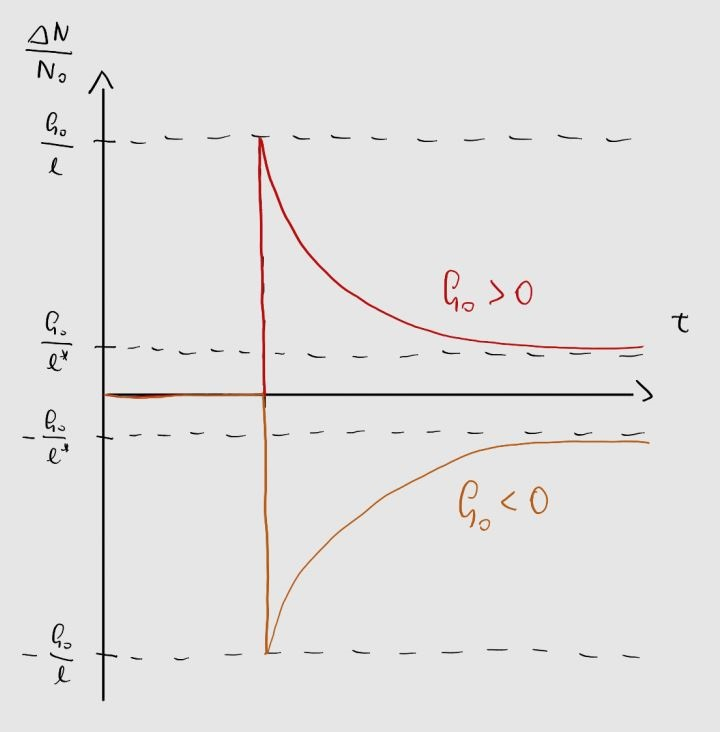
\includegraphics[width=0.6\textwidth]{img/impulsni.jpg}
  \caption{Závislost relativní změny četnosti neutronů pro impulsní charakteristiku.}
  \label{fig_impulsni}
\end{figure}

Je tedy jasné, že v čase $t=0$ je relativní změna četnosti neutronů ovlivněna okamžitými neutrony a v čase $t \rightarrow \infty$ zpožděnými neutrony. V reálu se u vysokých vložených reaktivit (TRIGA) výrazně projevují zpětné vazby. Výrazy platí pro záporné i kladné vnesené reaktivity.

\subsubsection{Přechodová charakteristika}

Jde o případ, kdy je vložená reaktivita konstantní, tedy:

$$\rho(t) = \rho_0$$

Lze aplikovat i v reálu (pád tyče), i když ve skutečnosti to tak není (tyč padá nějakou tu dobu). Pro řešení vycházíme ještě z doby před zavedením integrální podoby jednobodové kinetiky\footnote{Tady si pro další usnadnění života přepíšu proměnou v LT pomocí $z$, aby se mi nepletlo s obecným řešením.}:

$$ \tilde{N}(z) = \dfrac{N_0}{z} + \tilde{G_0}(z) \cdot \mathcal{L}[\rho(t) N(t)](z), $$

$$ \tilde{N}(z) = \dfrac{N_0}{z} + \rho_0 \tilde{G_0}(z) \tilde{N}(z).$$

Nás zajímá relativní četnost $\dfrac{\tilde{N}(z)}{N_0}$ a zároveň za $\tilde{G_0}(z)$ dosadíme z \eqref{prenosova_funkce}, tedy:

\begin{equation}
  \boxed{
  \dfrac{\tilde{N}(z)}{N_0} = \dfrac{1}{z \left ( 1-\rho_0 \tilde{G_0}(z) \right )} = \dfrac{\Lambda + \sum_{i = 1}^m \dfrac{\beta_{\text{ef},i}}{z + \lambda_i}}{z \left ( \Lambda + \sum_{i = 1}^m \dfrac{\beta_{\text{ef},i}}{z + \lambda_i} \right ) - \rho_0}.
  \label{prechodova_charakteristika_LT}}
\end{equation}

Rovnice \eqref{prechodova_charakteristika_LT} se dá transformovat úplně stejně, jako v minulé kapitole $\rightarrow$ převedu na parciální zlomky:

$$ \dfrac{\tilde{N}(z)}{N_0} = \sum_{n=0}^m \dfrac{C_n}{z-z_n}, $$

\begin{equation}
  \boxed{
  \dfrac{N(t)}{N_0} = \sum_{n=0}^m C_n e^{z_n t}.
  \label{prechodova_charakteristika}}
\end{equation}

Zaměříme-li se na znaménka koeficientů $C_n$ a $z_n$, tak:

\begin{itemize}
  \item $z_0$ má stejné znaménko jako $\rho_0$,
  \item $z_n < 0 \: \: \: \forall \: n \in \widehat{m}$,
  \item $C_0 > 0$,
  \item $C_n$ mají opačná znaménka než $\rho_0, \: \: \: \forall \: n \in \widehat{m}$.
\end{itemize}

Vztah mezi kořeny $z_n$ v závislosti na reaktivitě zobrazuje graf na obrázku \ref{fig_zn-rho}.

\begin{figure}[H]
  \centering
  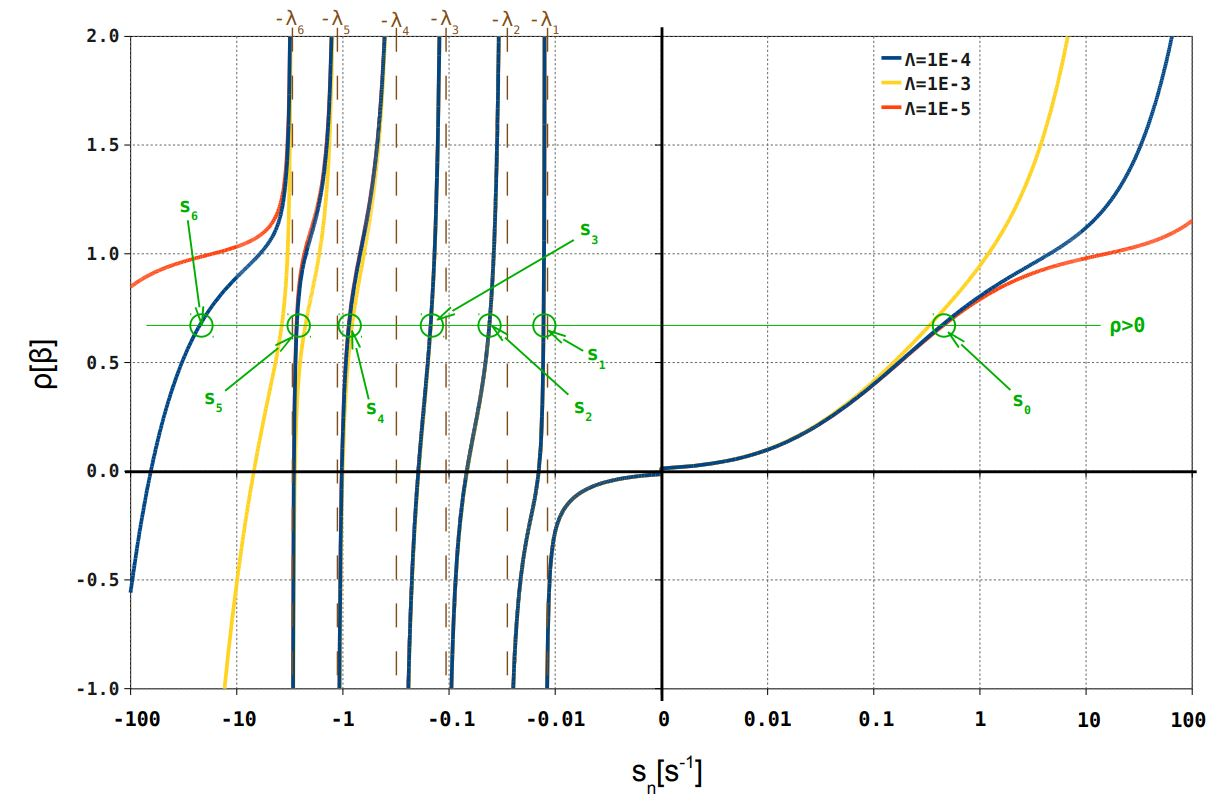
\includegraphics[width=1\textwidth]{img/zn-rho.jpg}
  \caption{Vztah mezi kořeny $z_n$ (zde $s_n$) a reaktivitou $\rho_0$ v přechodové charakteristice.}
  \label{fig_zn-rho}
\end{figure}

Pro $\rho_0 < 0$ bude relativní četnost v čase exponenciálně klesat (což bude ovlivněno největším $|z_n|$, což je závislé na $\Lambda$ $\rightarrow$ s menším $\Lambda$ očekáváme strmější nástup).

Pro $\rho_0 > 0$ po chvíli převládne kladné $z_0$ s $C_0$ a relativní četnost exponenciálně poroste. Do tohoto zlomového okamžiku bude relativní četnost také růst, ale s jiným průběhem.

Průběh relativní četnosti při vnesení kladné i záporné reaktivity zobrazuje obrázek \ref{fig_prechodova}.

\begin{figure}[H]
  \centering
  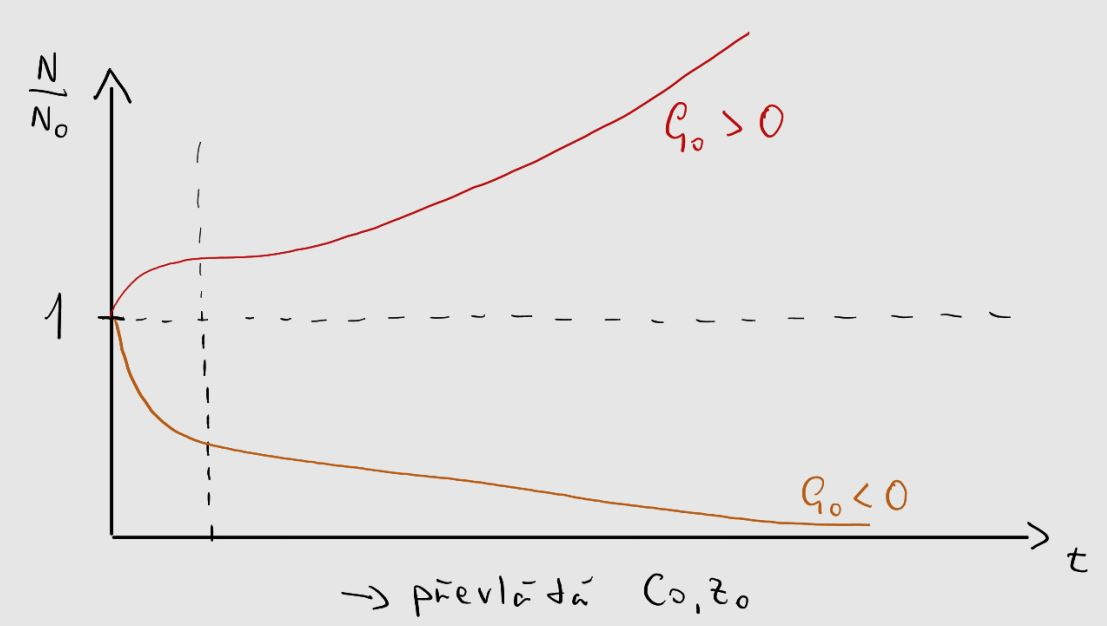
\includegraphics[width=0.7\textwidth]{img/prechodova.jpg}
  \caption{Závislost relativní četnosti neutronů pro přechodovou charakteristiku.}
  \label{fig_prechodova}
\end{figure}



\textbf{Ustálená perioda reaktoru}

Po vymizení všech členů, kdy bude vývoj ovlivněn pouze členy $z_0$ a $C_0$, bude možné popsat relativní četnost pomocí právě jedné exponenciály:

$$ \dfrac{N(t)}{N_0} = C_0 e^{z_0 t}. $$

Tento vztah je možné využít při vymizení většiny skupin zpožděnek, v tzv. \textbf{asymptotické oblasti} kdy už převládá pouze nejdelší ze skupin s $\tau_1 \approx 80$~s. Poté je možné stanovit tzv. \textbf{ustálenou periodu reaktoru} jako:

$$ T_e = \dfrac{1}{z_0}, $$

což při dosazení do vztahu, který jsme získali v minulé kapitole (při hledání kořenů $z_n$ pomocí položení jmenovatele nule)\footnote{Platí pro každé $z_n$, tedy i pro $z_0$}:

\begin{equation}
  \rho_0 = z_0 \left ( \Lambda + \sum_{i = 1}^m \dfrac{\beta_{\text{ef},i}}{z_0 + \lambda_i} \right )
  \label{rho0-z0}
\end{equation}

dává tzv. \textbf{in-hour equation}, tedy vztah, který dává do souvislosti reaktivitu a peroidu\footnote{Tohle jsme dělali právě na ERF, kdy jsme vložili kladnou reaktivitu a čekali, až se četnost začne zvyšovat podle jedné exponenciály. U té jsme poté určili její koeficient (směrnici v log měřítku) a po zadání do tohodle vztahu jsme zjistili hledanou kladnou reaktivitu.}:

\begin{equation}
  \boxed{
  \rho_0 = \dfrac{\Lambda}{T_e} + \sum_{i=1}^{m} \dfrac{\beta_{\text{ef},i}}{1 + \lambda_i T_e}.
  \label{in-hour}}
\end{equation}

\textbf{Zvláštní případy}

Podle velikosti reaktivity $\rho_0$ mohou nastat různé případy, které se limitně blíží k již odvozeným závěrům:

\textbf{a) Velmi malá reaktivita}

Pokud nastane případ, že $|\rho_0| << \beta_{\text{ef}}$, poté musí platit: $|z_0| << \lambda_1 << \lambda_2 ...$ . Díky tomu je možné ve výrazu \eqref{rho0-z0} odstranit $z_0$ ze zlomku a výraz se nám zjednodušší na:

$$ \rho_0 = \dfrac{1}{T_e} \left ( \Lambda + \sum_{i=1}^m \dfrac{\beta_{\text{ef},i}}{\lambda_i} \right ). $$

Závorka v tomto výrazu je již definovaná efektivní střední doba života neutronů a po vyjádření periody dostáváme:

$$ T_e^* = \dfrac{\ell^*}{\rho_0} \approx \dfrac{\ell^*}{k_{\text{ef}}-1}, $$

\noindent což je v podstatě důkaz již definované efektivní periody reaktoru. Pro malé reaktivity je tedy očividné, že se na reaktivitě a periodě systému výrazně podílí zpožděné neutrony.

\textbf{b) Velmi velká kladná reaktivita}

Pokud $\rho_0 >> \beta_{\text{ef}}$, platí, že $|z_0| >> \lambda_m << \lambda_{m-1} ...$ . V takovém případě je možné ze zlomku ve vztahu \eqref{rho0-z0} odstranit $\lambda_i$ a dostáváme:

$$ \rho_0 = \dfrac{\Lambda}{T_e} + \beta_{\text{ef}}. $$

Po úpravě a vyjádření periody:

$$ T_e = \dfrac{\Lambda}{\rho_0 - \beta_{\text{ef}}} = \dfrac{\ell}{k_{\text{ef}} \cdot (\rho_0 - \beta_{\text{ef}})} \approx \dfrac{\ell}{k_{\text{ef}}-1}. $$

Pro velké reaktivity tedy vymizí efekt zpožděných neutronů a perioda je dána pouze okamžitými (jak nečekané).

\textbf{c) Velmi velké záporné reaktivity}

Pokud $\rho_0 << -\beta_{\text{ef}}$, platí, že $|z_0| \approx -\lambda_1$\footnote{viz graf na obrázku \ref{fig_zn-rho}}. Poté je z definice ustálené periody reaktoru jasné, že:

$$ T_e = \dfrac{-1}{z_0} = \tau_1. $$

S libovolně malou vloženou reaktivitou není možné odstavovat reaktor pomaleji. Jsme tím schopni ovlivnit pouze rychlost okamžitého poklesu, ale tento doběh bude klesat vždy stejně rychle (řádově těch 80~s).

\textbf{d) Kritičnost na okamžitých neutronech}

Pokud $\rho_0 = \beta_{\text{ef}}$, pak se vrátíme zpět do rovnice \eqref{rovnice_kinetiky_zpozdenky_3}, která nám definovala produkční tvar rovnice jednobodové kinetiky se zpožděnými neutrony. Díky této rovnosti vymizí první člen a rovnice se změní na tvar:

$$ \dfrac{dN}{dt} = 0 + \sum_{i=1}^m \lambda_i C_i(t), $$

$$ \dfrac{dC_i}{dt} = -\lambda_i C_i(t) + \dfrac{\beta_{\text{ef},i}  N(t)}{\Lambda}. $$

Tato rovnice je řešitelná pomocí integračního faktoru (a dělat to nebudeme, je to ve skriptech\footnote{Možná když se budu nudit... :D}). Výsledkem je kritičnost bez potřeby zpožděných neutronů, tzv. kritičnost na okamžitých neutronech (propmt criticality), četnost exponenciálně roste, perioda se zkracuje.

\textbf{Periodické změny}

Nyní předpokládejme, že budeme střídavě měnit reaktivitu na $+ 0,5 \beta_{\text{ef}}$ a $- 0,5 \beta_{\text{ef}}$, viz obrázek \ref{fig_periodicke}.

\begin{figure}[H]
  \centering
  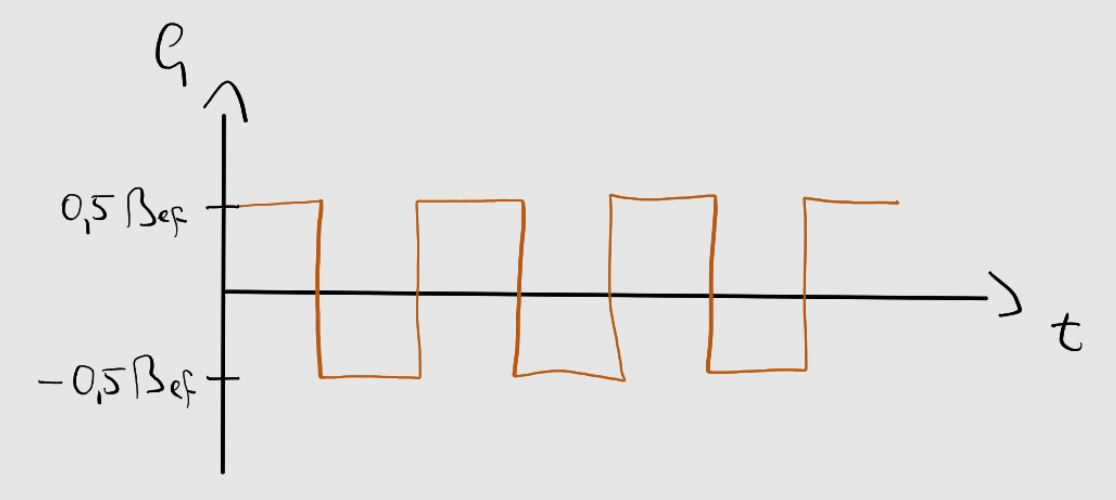
\includegraphics[width=0.5\textwidth]{img/periodicke.jpg}
  \caption{Ukázkový vstup pro periodickou změnu reaktivity.}
  \label{fig_periodicke}
\end{figure}

Poté ale pomocí již zmíněných vztahů pro periody dostáváme:

\begin{itemize}
  \item $+ 0,5 \beta_{\text{ef}} \rightarrow T_e = 10$~s,
  \item $- 0,5 \beta_{\text{ef}} \rightarrow T_e = 100$~s,
\end{itemize}

tedy relativní četnost musí růst rychleji, než klesat. Výsledkem tedy není periodická odezva četnosti, ale četnost postupně roste, viz obrázek \ref{fig_periodicke_reseni}.

\begin{figure}[H]
  \centering
  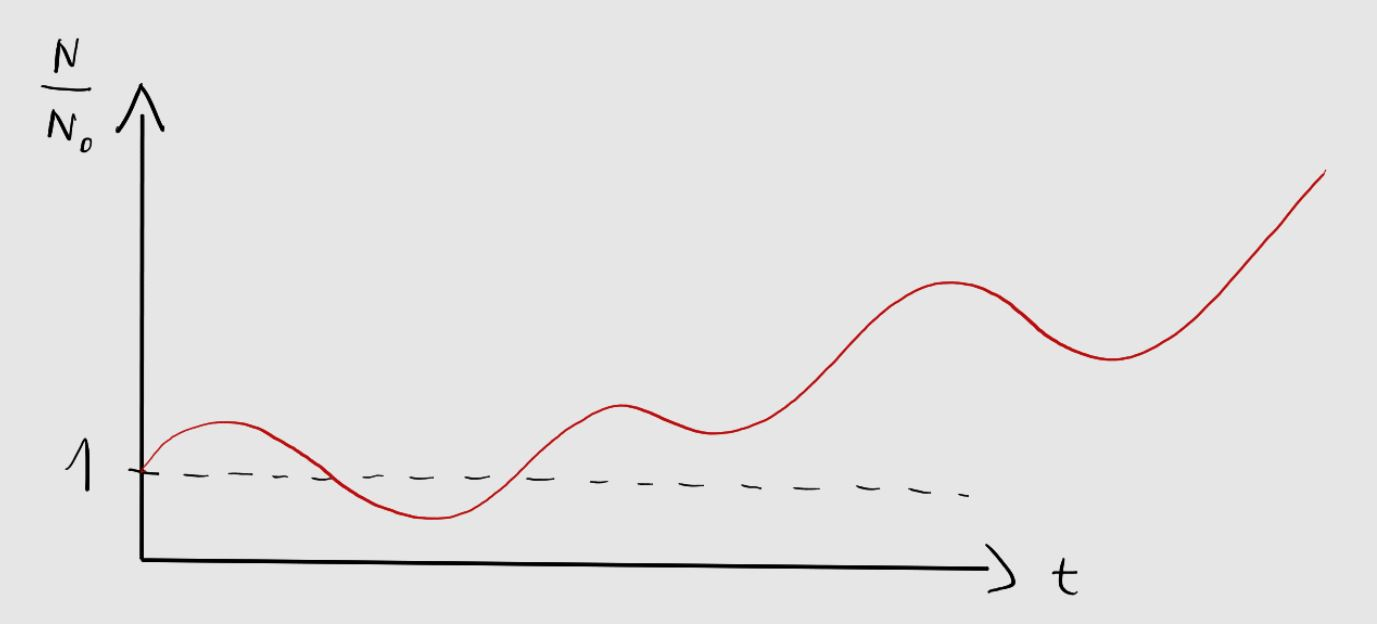
\includegraphics[width=0.5\textwidth]{img/periodicke_reseni.jpg}
  \caption{Ukázkový výstup pro periodickou změnu reaktivity.}
  \label{fig_periodicke_reseni}
\end{figure}

\textbf{Konstantní produkce zpožděných neutronů}

Jde o teoretický model, který lze očekávat v prvních desetinách vteřin po skokové změně reaktivity. Pro odvození opět skočíme do produkčního tvaru, kde předpokládáme, že máme produkční rovnováhu:

$$ \dfrac{dC_i}{dt} |_{0} = 0. $$

Rovnice tedy vypadají:

$$ \dfrac{dN}{dt} = \dfrac{\rho - \beta_{\text{ef}}}{\Lambda} N(t) + \sum_{i=1}^m \lambda_i C_i(t), $$

$$ 0 = -\lambda_i C_i(t) |_{0} + \dfrac{\beta_{\text{ef},i}  N(t)}{\Lambda}. $$

Obě rovnice jsou opět v pohodě řešitelné, ale ani to zde dělat nebudeme\footnote{To bych se musel fakt hodně nudit}. Řešení je ve skriptech a pro konstantní reaktivitu je tvaru:

$$ \dfrac{N(t)}{N_0} = \dfrac{\beta_{\text{ef}}}{\beta_{\text{ef}}-\rho_0} \left [ 1 - \dfrac{\rho_0}{\beta_{\text{ef}}} \exp{ \left ( \dfrac{\rho_0 - \beta_{\text{ef}}}{\Lambda}t \right ) } \right ]. $$

Tímto vztahem je tedy možné popsat průběh do inflexního bodu, který je dán parametrem $C_0$. Je zde možné nalézt paralelu s př. 3, kde se uvažovala pouze jedna skupina zpožděnek. Člen $C_0$ a $C_1$ zde vyšel stejně a exponenciela ve výraze představuje kořen $z_1$. Tato aproximace přibližuje odezvu pouze okamžitých neutronů.

Koeficient $C_0$:

$$ C_0 = \dfrac{\beta_{\text{ef}}}{\beta_{\text{eff}} - \rho_0} $$

představuje absolutní hodnotu relativní četnosti neutronů při okamžité změně reaktivity, viz graf na obrázku \ref{fig_konstantni_produkce}.

\begin{figure}[H]
  \centering
  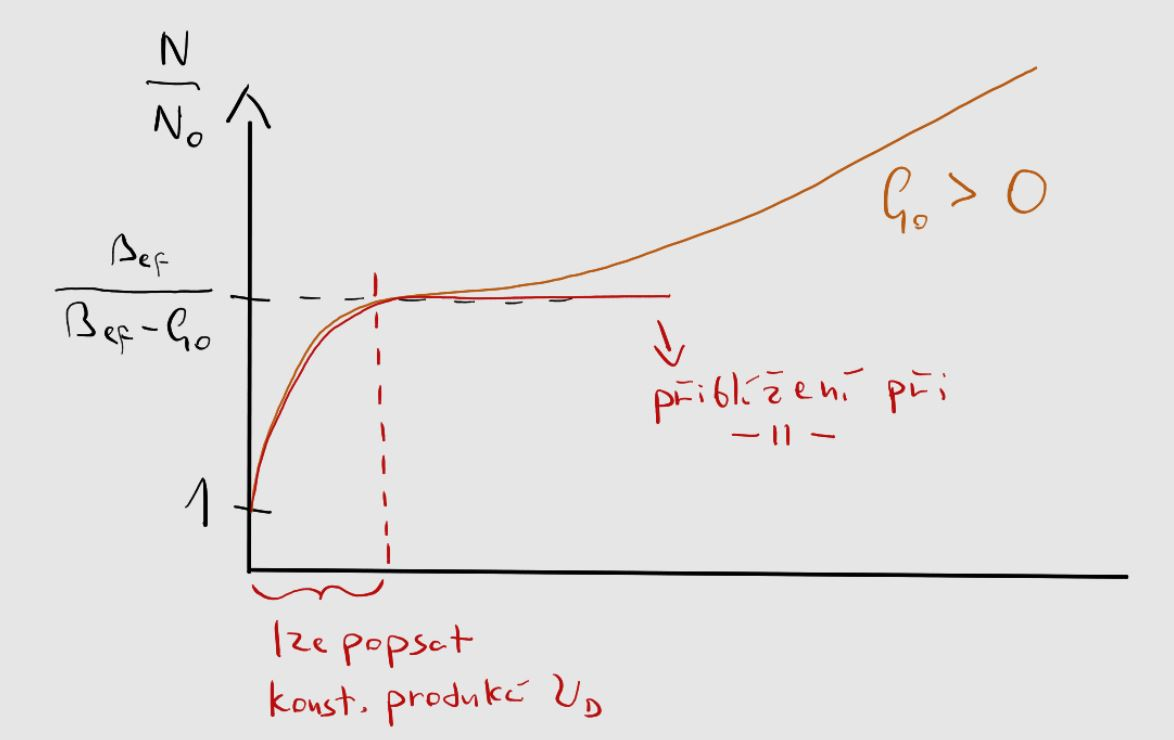
\includegraphics[width=0.5\textwidth]{img/konstantni_produkce.jpg}
  \caption{Průběh relativní četnosti při konstantní produkci zpožděných neutronů (červená křivka) vs. skutečný průběh (oranžová).}
  \label{fig_konstantni_produkce}
\end{figure}

\textbf{Okamžitý skok}

Další možnou aproximací je metoda okamžitého skoku, kdy v čase $t = 0$ předpokládáme:

$$ \dfrac{dN}{dt} = 0. $$

Tuto metodu lze aplikovat až po prvních pár desetinách vteřiny, kdy odezní vliv okamžitých neutronů, tedy v momentě, kdy se nacházíme za inflexním bodem\footnote{Metoda konstantní produkce neutronů se dá použít před inflexním bodem a metoda okamžitého skoku po inflexním bodu.}. Jde o aproximaci přibližující vliv zpožděných neutronů.

Následující vztahy jsou odvozeny pouze pro 1 skupinu zpožděných neutronů\footnote{Metoda konstantní produkce zpožděných neutronů vyjadřuje chování v systému díky okamžitým neutronům, proto nebylo potřeba uvažovat různé skupiny zpožděnek. Metoda okamžitého skoku naopak vyjadřuje vliv zpožděných neutronů, ovšem vztahy pro $m$ skupin by byl složitý.} a pro konstantní reaktivitu, přičemž odvození je opět ve skriptech\footnote{To bych se musel fakt hodně nudit.}. Řešíme rovnice tvaru:

$$ 0 = \dfrac{\rho - \beta_{\text{ef}}}{\Lambda} N(t) + \bar{\lambda} C(t), $$

$$ \dfrac{dC}{dt} = -\bar{\lambda} C(t) + \dfrac{\beta_{\text{ef}}  N(t)}{\Lambda}, $$

které dávají řešení:

$$ \dfrac{N(t)}{N_0} = \dfrac{\beta_{\text{ef}}}{\beta_{\text{ef}} - \rho_0} \exp{\left ( \dfrac{\bar{\lambda} \rho_0}{\beta_{\text{ef}} - \rho_0} t \right )}. $$

Je opět možné nalézt paralelu s př. 3, jelikož exponenciála představuje kořen $z_0$ a člen před exponencielou koeficient $C_0$, viz graf na obrázku \ref{fig_okamzity_skok}.

\begin{figure}[H]
  \centering
  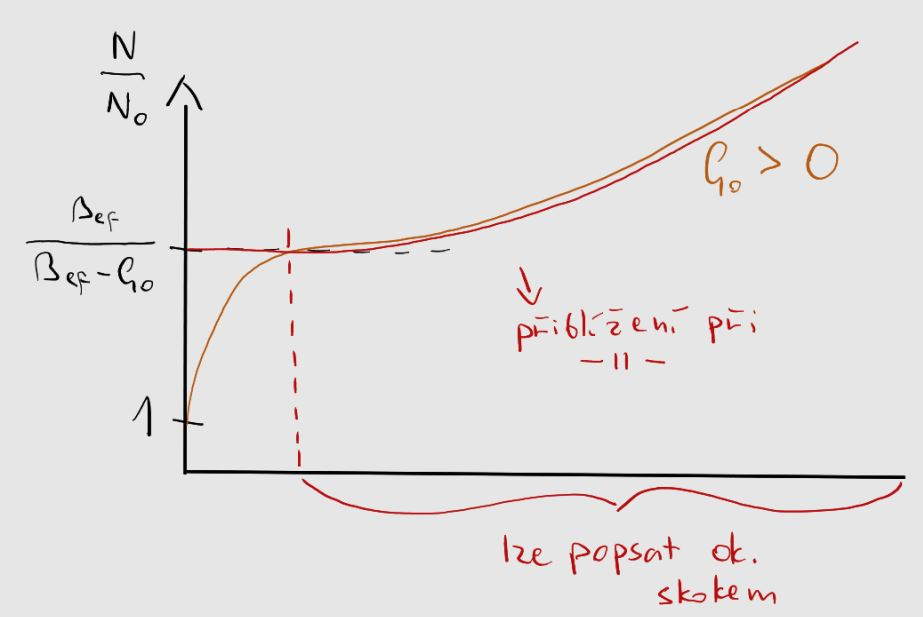
\includegraphics[width=0.5\textwidth]{img/okamzity_skok.jpg}
  \caption{Průběh relativní četnosti při okamžitém skoku (červená křivka) vs. skutečný průběh (oranžová).}
  \label{fig_okamzity_skok}
\end{figure}

Ve skutečnosti je přiblížení jednou skupinou dost mimo a je vhodnější k popisu použít více skupin. Příklad je pouze demonstrační\footnote{Nebo by bylo vhodnější středovat $\bar{\lambda}$ pomocí $\tau_i$.}.

\textbf{Externí zdroj neutronů}

Externí zdroj neutronů je dobré využívat k bezpečnějšímu spouštění, jelikož dává silnější tok než pozadí, které umožňuje sledovat kvalitnější odezvu na detektorech\footnote{Pozadí, resp. samoštěpení by šlo ke spuštění použít také, ale bylo by zapotřebí kvalitnější detektory, který by poskytly kvalitní odezvu a spouštění bylo skutečně bezpečné.}. Četnost neutronů při zavedení externího zdroje a pro různé reaktivity systému zobrazuje graf na obrázku \ref{fig_zdroj}.

\begin{figure}[H]
  \centering
  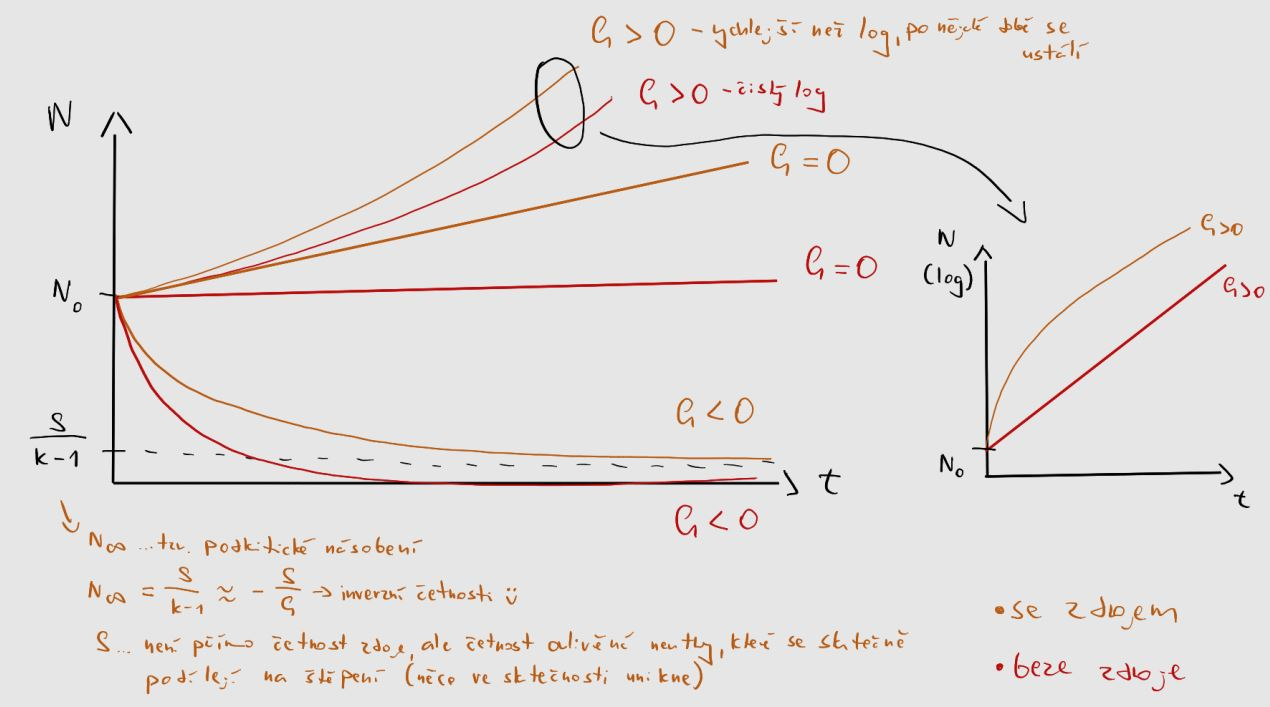
\includegraphics[width=0.8\textwidth]{img/zdroj.jpg}
  \caption{Četnost neutronů pro různé reaktivity s externím zdrojem (oranžová křivka) a bez externího zdroje (červená).}
  \label{fig_zdroj}
\end{figure}

\textbf{Podmínka stability s externím zdrojem:}

Mějme externí zdroj neutronů a sledujeme, za jakých podmínek se četnost neutronů ustálí. Vyjdeme z produkčního tvaru jednobodové kinetiky (kam dosadíme externí zdroj neutronů $S(t)$) kde předpokládáme ustálený tvar, tedy při dosazení $N(t) = N_0$ a $C_i(t) = C_i^0$ (jde o konstanty $\rightarrow$ nulové derivace) dostáváme tvar:

$$ 0 = \dfrac{\rho(t) - \beta_{\text{ef}}}{\Lambda} N_0 + \sum_{i=1}^m \lambda_i C_i^0 + S(t), $$

$$ 0 = -\lambda_i C_i^0 + \dfrac{\beta_{\text{ef},i}  N_0}{\Lambda}. $$

Rovnice do sebe podosazujeme a dostáváme jednoduché řešení (podmínka stability):

$$ 0 = \dfrac{\rho(t)}{\Lambda} N_0 + S(t). $$

Aby stabilita nastala, musí uvedená rovnice platit. K tomu dojde pouze za předpokladu:

\begin{itemize}
  \item $S(t) = 0$, $\rho(t) = 0$ $\rightarrow$ máme kritický stav a vypnutý zdroj,
  \item $S(t) = 0$, $N_0 = 0$ $\rightarrow$ máme vypnutý reaktor, v praxi zřejmě nedosažitelné,
  \item $S(t) > 0$, $\rho(t) = -S(t) \dfrac{\Lambda}{N_0}$ $\rightarrow$ hledaná podmínka stability pro zapnutý externí zdroj\footnote{Toho jsme využili u metody inverzních četností v ERF, kdy se určovala vnesená reaktivita.}.
\end{itemize}

\textbf{Vztah mezi dvěmi stavy:}

Nyní předpokládejme, že máme stav s $N_1$, $\rho_1$ a $S_1$, a změnou reaktivity docílíme nového stavu s $N_2$, $\rho_2$ a $S_2$. Zajímá nás vztah mezi $N_1$ a $N_2$ v závislosti na reaktivitách $\rho_{1,2}$ a externích zdrojích $S_{1,2}$. Předpokládejme, že ke změnám došlo okamžitě, proto můžeme aplikovat metodu konstantní produkce zpožděných neutronů i metodu okamžitého skoku (zde si pomůžeme přiblížením $C_i^1(t) = C_i^2(t)$). Schematicky by šel přechod znázornit pomocí grafu na obrázku \ref{fig_podil_N_ukazka}.

\begin{figure}[H]
  \centering
  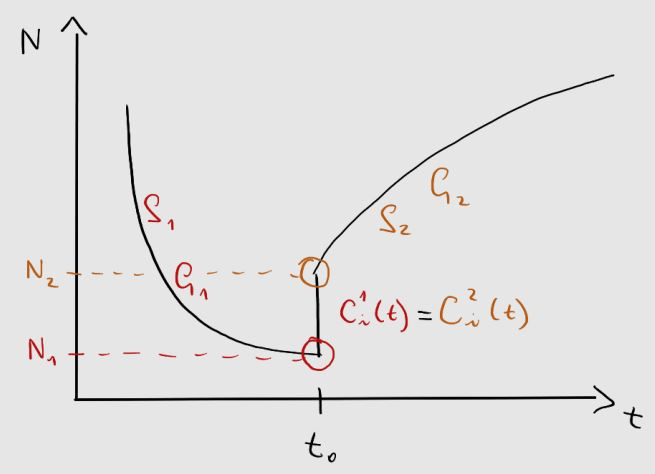
\includegraphics[width=0.5\textwidth]{img/podil_N_ukazka.jpg}
  \caption{Znázornění příkladu pro odvození vztahu mezi dvěmi stavy.}
  \label{fig_podil_N_ukazka}
\end{figure}

Vyjdeme z produkčního tvaru rovnic kinetiky (ale pouze z první rovnice, zpožděnky nás nezajímají), kterou si zapíšeme pro oba stavy a sečteme (obě strany jsou nulové). Dostáváme jednu rovnici:

$$ \dfrac{\rho_1 - \beta_{\text{ef}}}{\Lambda} N_1 + \sum_{i=1}^m \lambda_i C_i(t) + S_1 = \dfrac{\rho_2 - \beta_{\text{ef}}}{\Lambda} N_2 + \sum_{i=1}^m \lambda_i C_i(t) + S_2. $$

Po úpravě a vyjádření získáme:

$$ \dfrac{N_2}{N_1} = \dfrac{\beta_{\text{ef}} - \rho_1}{\beta_{\text{ef}} - \rho_2} + \dfrac{\Lambda}{N_1} \dfrac{S_2 - S_1}{\beta_{\text{ef}} - \rho_2}. $$

Toto přiblížení, přestože je jeho odvození dosti nepřesné a idealistické dává kupodivu přesné výsledky. Předvedeme na pár příkladech.

Mějme kritický stav ($\rho_1 = 0$) s externím zdrojem $S_1$. V jistém momentu zdroj vypneme (ve stavu s aktuální četností $N_1$), čímž se dostáváme do stavu s $\rho_2 = 0$ (stále máme kritický stav, četnost ovlivňujeme pouze pomocí zdroje), $S_2 = 0$ a $N_2$. Kupodivu, $N_2$ se neustálí ihned na pozici jako předchozí $N_1$, ale skočí na nižší hladinu, přesně podle rovnice:

$$ \dfrac{N_2}{N_1} = 1 - \dfrac{\Lambda}{N_1} \dfrac{S_1}{\beta_{\text{ef}}}. $$

Tento jev je možné fyzikálně odůvodnit tak, že v momentě vypnutí zdroje vznikají zpožděnky z předchozích generací, kdy ještě četnost nebyla tak vysoká (nižší než ve stavu $N_1$). Je jich tedy výrazně méně a nejsou schopny kompenzovat nedostatek v aktuální generaci, viz obrázek \ref{fig_podil_N_1}.

\begin{figure}[H]
 \centering
 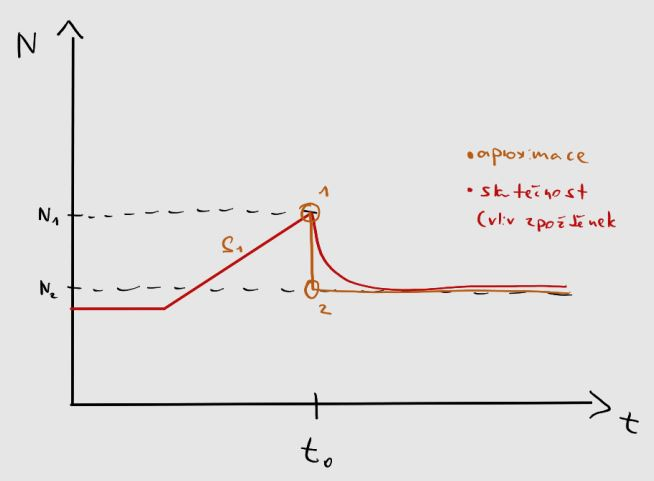
\includegraphics[width=0.6\textwidth]{img/podil_N_1.jpg}
 \caption{První ukázka využití vztahu mezi dvěmi stavy ($S_1$).}
 \label{fig_podil_N_1}
\end{figure}

Dalším příkladem může být zvyšování četnosti pomocí reaktivity. Mějme reaktor bez zdrojů ($S_{1,2} = 0$) a stav s malinkatou reaktivitou $\rho_1$. Opět v jistém momentě s četností $N_1$ vrátíme reaktivitu do stavu $\rho_2 = 0$, přičemž nová četnost opět skokově klesne dle vztahu:

$$ \dfrac{N_2}{N_1} = \dfrac{\beta_{\text{ef}} - \rho_1}{\beta_{\text{ef}}}. $$

Zdůvodnění je zde stejné, viz graf na obrázku \ref{fig_podil_N_2}.

\begin{figure}[H]
 \centering
 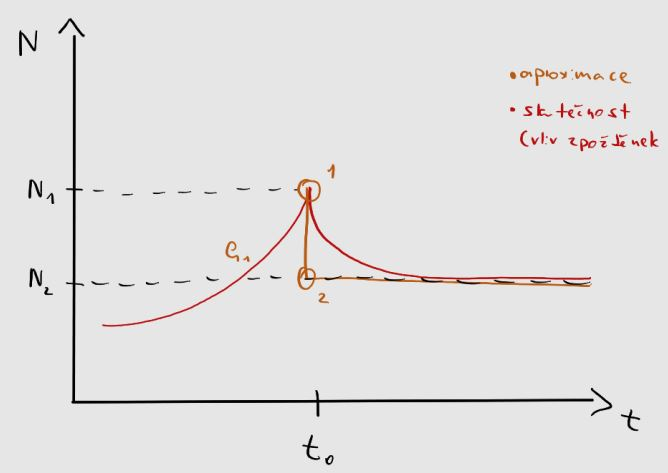
\includegraphics[width=0.6\textwidth]{img/podil_N_2.jpg}
 \caption{Druhá ukázka využití vztahu mezi dvěmi stavy ($\rho_1$).}
 \label{fig_podil_N_2}
\end{figure}

Z praktického hlediska je výhodnější najíždět mezi stavy postupně a nikoliv skokově. Díky tomu nebudeme sledovat skokové změny četností.

\subsubsection{Frekvenční charakteristika}

Pro odvození frekvenční charakteristiky je třeba trochu více matematiky.

\textbf{Přenosová funkce nulového reaktoru}

Platí, že každý lineární systém (takový, který je možné popsat soustavou lineárních diferenciálních rovnic) je možné popsat pomocí tzv. \textbf{přenosové funkce nulového reaktoru} $\tilde{W_{yx}}(s)$ definované dle:

\begin{equation}
  \boxed{
  \tilde{W_{yx}}(s) \equiv \dfrac{\tilde{y}(s)}{\tilde{x}(s)},
  \label{prenosova_funkce_definice}}
\end{equation}

kde:

\begin{itemize}
  \item $\tilde{y}(s)$ představuje výstupní veličinu (v našem případě jde o $\tilde{N}(s)$, resp. po převodu $N(t)$),
  \item $\tilde{x}(s)$ představuje vstupní veličinu (v našem případě $\tilde{\rho}(s)$, resp. $\rho(t)$).
\end{itemize}

Poté naši hledanou výstupní funkci nalezneme dle:

$$ \tilde{y}(s) = \tilde{W_{yx}}(s) \cdot \tilde{x}(s). $$

Jedná se o součin dvou Laplaceovsky transformovaných funkcí, tudíž po převedení se jedná o jejich konvoluci:

$$ y(t) = (W_{yx} * x ) (t) = \int_0^t W_{yx}(t-t') x(t') dt'. $$

Pro výpočet potřebujeme znát originální přenosovou funkci, kterou získáme pomocí Laplaceova obrazu\footnote{Ti, co dávali o RMF pozor si všimnou, že se jedná o Greenovu funkci.}:

$$ W_{yx}(t) \equiv \mathcal{L}^{-1}[\tilde{W_{yx}}(s)](t). $$

\textbf{Linearizovaný model}

Jaderný reaktor ale ve skutečnosti není lineárním systémem. Podíváme-li se na rovnici kinetiky v integrálním tvaru (viz \eqref{integralni_kinetika}), všimneme si, že se v integrandu vyskytuje součin vstupní ($\rho(t)$) a výstupní ($N(t)$) veličiny\footnote{Nejde ji napasovat do konvoluce s přenosovou funkcí, kterou jsme si definovali před chvílí.}:

$$ N(t) = N_0 + \int_0^t G_0(t-t') \rho(t') N(t')dt'. $$

Proto musíme rovnici linearizovat. To provedeme, zavedeme-li odchylku $\Delta N(t)$ jako:

$$ \Delta N(t) = N(t) - N_0 $$

a tu dosadíme do integrálního tvaru \eqref{integralni_kinetika}. Výsledkem bude:

$$ \Delta N(t) = N_0 \int_0^t G_0(t-t') \rho(t') dt' + \int_0^t G_0(t-t') \rho(t') \Delta N(t')dt'. $$

Právě ten druhý člen představuje nelinearitu systému. Zavedeme-li předpoklady, že se jedná o malé změny $\rho$ a malé změny $\Delta N$, můžeme druhý člen vypustit a dostaneme linearizovaný tvar:

\begin{equation}
  \boxed{
  \Delta N(t) = N_0 \int_0^t G_0(t-t') \rho(t') dt'.
  \label{linearizovana_kinetika}}
\end{equation}

Podobného výsledku jsme dosáhli už v impulsní charakteristice, ale tam jsme museli předpokládat okamžitý skok pomocí Diracovy funkce. Zde je to o něco málo obecnější a za $\rho(t)$ jde dosazovat víceméně cokoliv.

Odtud přejdeme opět zpět k LT pomocí konvoluce a dostáváme:

$$ \Delta \tilde{N}(s) = N_0 \tilde{G_0}(s) \tilde{\rho} (s), $$

což pokud chceme dokázat, že se jedná o lineární systém, chceme dostat do stejného tvaru, jako jsme si definovali přenosovou funkci nulového reaktoru (výstupní/vstupní). Zároveň za $\tilde{G_0}(s)$ můžeme dosadit z definice \eqref{prenosova_funkce}, čímž dostaneme:

$$ \tilde{G_0}(s) = \dfrac{1}{N_0} \dfrac{\Delta \tilde{N}(s)} {\tilde{\rho}(s)} = \dfrac{1}{s \left ( \Lambda + \sum_{i=1}^m \dfrac{\beta_{\text{ef},i}}{\lambda_i + s} \right )}.$$

\textbf{Frekvenční charakteristika -- konečně}

Nyní můžeme konečně řešit frekvenční charakteristiku, tedy předpoklad, že máme periodicky se měnící reaktivitu:

$$ \rho(t) = \rho_0 \cos (\omega t), $$

což v LT znamená:

$$ \tilde{\rho}(s) = \dfrac{s}{s^2 + \omega^2}. $$

Zajímá nás relativní změna četnosti, tedy:

$$ \dfrac{\Delta \tilde{N}(s)}{N_0} = \tilde{\rho}(s) \tilde{G_0}(s) = \rho_0 \: \dfrac{s}{s^2 + \omega^2} \: \dfrac{1}{s \left ( \Lambda + \sum_{i=1}^m \dfrac{\beta_{\text{ef},i}}{\lambda_i + s} \right )} = \rho_0 \: \dfrac{1}{s^2 + \omega^2} \: \dfrac{1}{\Lambda + \sum_{i=1}^m \dfrac{\beta_{\text{ef},i}}{\lambda_i + s}}. $$

Jde opět o lomenný výraz, tudíž ho můžeme převést na parciální zlomky\footnote{Nyní opět použijeme koeficienty $A_n$ a kořeny $s_n$, jelikož je tu jistá paralela s impulsní charakteristikou.}. Výraz má celkem $m+2$ kořenů. Prvních $m$ známe, jsou to ty záporné z impulsní charakteristiky. Zbylé dva kořeny jsou imaginární\footnote{Jako imaginární jednotku značíme $j$.}:

\begin{itemize}
  \item $s_n < 0 \: \: \: \forall \: n \in \widehat{m}$, navíc jsou stejné jako v impulsní charakteristice,
  \item $s_{m+1} = \omega j$,
  \item $s_{m+2} = - \omega j$.
\end{itemize}

Podle kuchařky dostaneme celkové řešení tvaru:

$$ \dfrac{\Delta \tilde{N}(s)}{N_0} = \sum_{n = 1}^{m+2} \dfrac{A_n}{s-s_n}, $$

$$ \dfrac{\Delta N(t)}{N_0} = \sum_{n = 1}^{m+2} A_n e^{s_n t}. $$

Díky zápornosti prvních $m$ členů první členy po čase vymizí a zůstanou pouze členy $m+1$ a $m+2$. Jejich kořeny jsou ryze imaginární $\rightarrow$ vede na řešení v goniometrických funkcích. Po trošce matematiky (substituci $s = \omega j$ a předpokladu\footnote{Resp. znalosti, prý to tak fakt je.}, že $\tilde{G_0}(\omega j)$ je komplexně sdružená funkce) dostaneme vyjádření koeficientů $A_{m+1}$ a $A_{m+2}$:

$$ A_{m+1} = \dfrac{\rho_0}{2} \tilde{G_0}(\omega j), $$
$$ A_{m+2} = \dfrac{\rho_0}{2} \tilde{G_0}(-\omega j), $$

tedy:

$$ \dfrac{\Delta N(t)}{N_0} \approx = \rho_0 \left [\dfrac{1}{2} \tilde{G_0}(\omega j) e^{\omega j t} + \dfrac{1}{2} \tilde{G_0}(-\omega j) e^{-\omega j t} \right ], $$

což je ve finále možné vyjádřit pomocí fázového posuvu $\varphi$:

\begin{equation}
  \boxed{
  \dfrac{\Delta N(t)}{N_0} = \rho_0 | \tilde{G_0}(\omega j) | \cos (\omega t + \varphi),
  \label{frekvencni_charakteristika_reseni}}
\end{equation}

kde pro $\varphi$ platí:

\begin{equation}
  \boxed{
  \varphi = \text{arctg} \left ( \dfrac{\text{Im} (\tilde{G_0}(\omega j)}{\text{Re}(\tilde{G_0}(\omega j)} \right ).
  \label{frekvencni_charakteristika_faze}}
\end{equation}

Co to tedy znamená? Máme-li periodickou změnu reaktivity, tak dostáváme periodickou odezvu na četnosti, která je ovšem posunutá o fázový posuv $\varphi$, viz graf na obrázku \ref{fig_frekvencni}.

\begin{figure}[H]
 \centering
 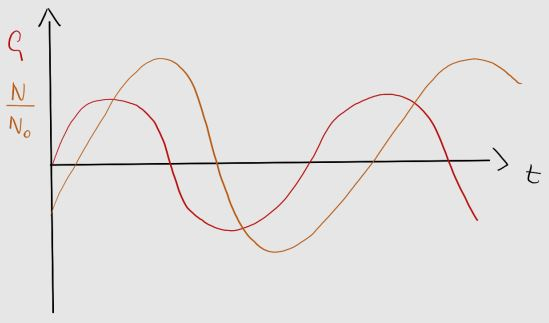
\includegraphics[width=0.5\textwidth]{img/frekvencni.jpg}
 \caption{Závislost relativní změny četnosti neutronů pro frekvenční charakteristiku a fázový posuv mezi odezvou a změnou reaktivity.}
 \label{fig_frekvencni}
\end{figure}

Absolutní hodnota je závislá pouze na frekvenci $\omega$ a vlastnostech reaktoru ($\Lambda$, $\lambda_i$ atd.). Ve skutečnosti ale maximální hodnota četnosti roste (viz obrázek \ref{fig_periodicke_reseni}). Tato nesrovnalost je způsobena právě linearizací systému. Toto přiblížení je tedy možné použít pouze pro kratší časy nebo menší reaktivity, kdy se nestihne rozvinout exponenciální odezva.

Pokud by nás zajímalo, jak vypadá závislost mezi frekvencí a aplitudou, resp. fázovým posuvem, stačí se juknout na graf na obrázku \ref{fig_frekvencni_zavislost}.

\begin{figure}[H]
  \centering
  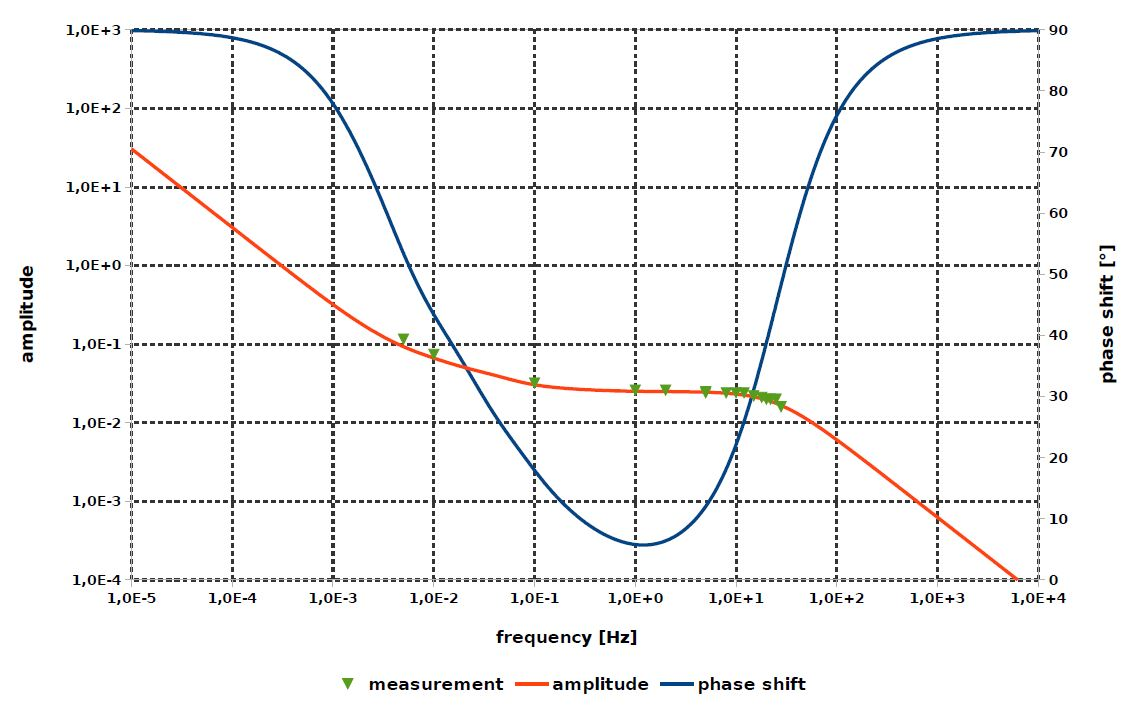
\includegraphics[width=1\textwidth]{img/frekvencni_zavislost.jpg}
  \caption{Závislost mezi frekvencí a amplitudou, resp. fázovým posuvem u frekvenční charakteristiky.}
  \label{fig_frekvencni_zavislost}
\end{figure}

Důkaz pro závislost amplitudy (která je ovlivněna $|\tilde{G_0}(\omega)|$) zde:

\textbf{a) Oblast pomalých změn:}

Tedy oblast s malými $\omega$, tedy i s malými $s$. V takovém případě můžeme v přenosové funkci zanedbat $s$ ve zlomku v sumě:

$$ \tilde{G_0}(s) = \dfrac{1}{s \left ( \Lambda + \sum_{i=1}^m \dfrac{\beta_{\text{ef},i}}{\lambda_i + s} \right )} \approx \dfrac{1}{s \left ( \Lambda + \sum_{i=1}^m \dfrac{\beta_{\text{ef},i}}{\lambda_i} \right )} = \dfrac{1}{s \ell^*} = \dfrac{1}{j \omega \ell^*} = - \dfrac{j}{\omega \ell^*}. $$

Tedy pro amplitudu:

$$ |\tilde{G_0}(\omega)| = \dfrac{1}{\omega \ell^*}. $$

A speciální případ (kvůli grafu):

$$ \left |\tilde{G_0} \left ( \dfrac{\beta_{\text{ef}}}{\ell^*} \right ) \right | = \dfrac{1}{\beta_{\text{ef}}}. $$

\textbf{b) Oblast rychlých změn:}

Zde můžeme ze stejného zlomku odstranit $\lambda_i$, potom dostaneme:

$$ \tilde{G_0}(s) = \dfrac{1}{s \left ( \Lambda + \sum_{i=1}^m \dfrac{\beta_{\text{ef},i}}{\lambda_i + s} \right )} \approx \dfrac{1}{s \left ( \Lambda + \sum_{i=1}^m \dfrac{\beta_{\text{ef},i}}{s} \right )} = \dfrac{1}{s \ell} = \dfrac{1}{j \omega \ell} = - \dfrac{j}{\omega \ell}. $$

Speciální případ:

$$ \left |\tilde{G_0} \left ( \dfrac{\beta_{\text{ef}}}{\ell} \right ) \right | = \dfrac{1}{\beta_{\text{ef}}}. $$

\textbf{c) Oblast středně rychlých změn:}

Zde můžeme\footnote{Z neznámých důvodů.} odstranit z výrazu $\Lambda$ a dostaneme:

$$ \tilde{G_0}(s) = \dfrac{1}{s \left ( \Lambda + \sum_{i=1}^m \dfrac{\beta_{\text{ef},i}}{\lambda_i + s} \right )} \approx \dfrac{1}{s \left ( \sum_{i=1}^m \dfrac{\beta_{\text{ef},i}}{\lambda_i + s} \right )} = \dfrac{1}{\sum_{i=1}^m \dfrac{\beta_{\text{ef},i}}{1 + \dfrac{\lambda_i}{s}} }. $$

Za předpokladu, že $\dfrac{\lambda_i}{s} \rightarrow 0$ dostáváme:

$$ \left |\tilde{G_0} \left (\omega \right ) \right | = \dfrac{1}{\beta_{\text{ef}}}. $$

Sumasumárum, závislost amplitudy na frekvenci (spočtenou vs. skutečnou) zobrazuje graf na obrázku \ref{fig_amplituda_frekvence}.

\begin{figure}[H]
  \centering
  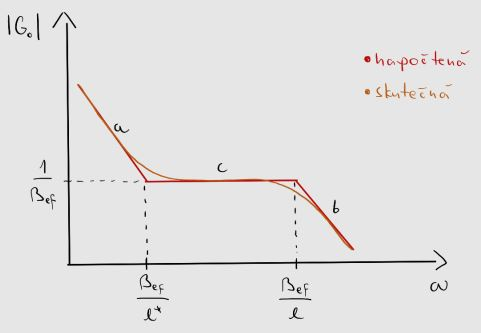
\includegraphics[width=0.5\textwidth]{img/amplituda_frekvence.jpg}
  \caption{Spočtená (červená) vs. napočtená (oranžová) závislost amplitudy na frekvenci při frekvenční charakteristice.}
  \label{fig_amplituda_frekvence}
\end{figure}

\subsubsection{Vlivy zjendnodušení}

Na závěr se podíváme, v jakých oblastech změn reaktivity můžeme použít různá zjednodušení v rovnicích jednobodové kinetiky.

\textbf{Zanedbání zpožděnek}

Zajímá nás, v jaké oblasti funguje jednobodová kinetika při zanedbání zpožděných neutronů. Dosadíme odchylku $\Delta N(t)$ do rovnice bodové kinetiky a s jediným zanedbáním malé změny reaktivity:

$$ \dfrac{d (\Delta N)}{dt} = \dfrac{k_{\text{ef}}-1}{\ell} (N_0 + \Delta N) \doteq \dfrac{\rho}{\ell} N_0. $$

Rovnici zLaplaceujeme a dostaneme:

$$ \tilde{\Delta N} = \dfrac{N_0}{\ell} \dfrac{\tilde{\rho}}{s}. $$

Dosadíme do definice přenosové funkce:

$$ \tilde{G_0}(s) = \dfrac{\tilde{\Delta N}}{N_0 \rho} = \dfrac{1}{s \ell}. $$

Toto je v podstatě to samé, co jsme získali v oblasti rychlých změn frekvenční charakteristiky. To tedy znamená, že toto přiblížení (bez zpožděnek) platí právě pro oblast rychlých změn reaktivity.

\textbf{Efektivní doba života neutronů}

Co se stane, pokud zaměníme $\ell$ za $\ell^*$? Odvození stejné, pouze dosadím nakonec $\ell^*$, zjednodušení tedy platí v oblasti pomalých změn reaktivity.

\textbf{Konstantní produkce zpožděnek}

V takovém případě je možné popsat systém pomocí jedné rovnice:

$$ \dfrac{dN}{dt} = \dfrac{\rho(t) - \beta_{\text{ef}}}{\Lambda} N(t) + \dfrac{\beta_{\text{ef}}}{\Lambda} N_0. $$

Stejným způsobem zavedeme odchylky a zlinearizujeme

$$ \dfrac{d (\Delta N)}{dt} = \dfrac{\rho(t)}{\Lambda} P_0 - \dfrac{\beta_{\text{ef}}}{\Lambda} \Delta N. $$

Zlaplaceujeme, dosadíme opět do přenosové funkce a máme:

$$ \tilde{G_0} (s) = \dfrac{1}{\Lambda s +  \beta_{\text{eff}}}. $$

Tento vztah je možné získat i z přímé definice přenosové funkce, při $\lambda_i \rightarrow 0$. Toto zjednodušení platí v oblasti rychlých a částečně rychlých změn.

\textbf{Okamžitý skok}

Složitá rovnice, vynecháme. Ve výsledku dostaneme:

$$ \tilde{G_0} (s) = \dfrac{s+\bar{\lambda}}{s \beta_{\text{eff}}}. $$

Toto je možné použít v oblasti malých změn a pomalých přechodových procesech.
\section[Zpětné vazby]{Zpětné vazby v jaderném reaktoru, principy jejich působení a důsledky pro dynamiku jaderného reaktoru}

\textbf{Zpětná vazba} (ZV) = proces, díky kterému se změna výstupních parametrů ($P$, $\Phi$) může podílet na změnu vstupních parametrů.

\textbf{Dynamika reaktoru} = to samé co kinetika, pouze už uvažuje zapojení ZV.

Cílem dynamiky reaktorů je řešit ZV. Vlivem ZV se nám totiž reaktivita mění (teplota, tlak, roztažnost...). Vše je primárně ovlivněno teplotou, jelikož s rosroucí reaktivitou roste výkon a tím i teplota systému. Celkovou reaktivitu můžeme určit jako součet reaktivity dodané zvenčí (tyče, palivo, konfigurace) a reaktivity ve ZV.

\subsection{Zpětné vazby}

ZV mohou být obecně:

\begin{itemize}
  \item kladné -- odezva roste, nestabilita.
  \item záporné -- odezva klesá, čímž se reaktor může stabilizovat,
\end{itemize}

Pokud se do reaktoru zavede kladná reaktivita s vlivem kladné zpětné vazby, a zároveň není-li reaktivita potlačena (tyčemi apod.), může i tato malá změna vést k nekontrolovanému nárůstu výkonu (rychlejší než exponenciální). Naopak, projeví-li se záporná zpětná vazba, reaktor se po chvíli stabilizuje. A na jaké hodnotě? Tehdy, pokud se reaktivity vyrovnají (kladná vnesená reaktivita se vyrovná záporné reaktivitě vziklé vlivem ZV $\rightarrow$ Celkový efekt je na nule), což závisí na velikosti vnesené reaktivity a velikosti zpětnovazebních koeficientů. Záporné ZV pomáhají k řízení reaktoru, jelikož vždy působí proti počáteční změně a mají tendenci reaktor stabilizovat, viz graf \ref{ZV}.

\begin{figure}[H]
  \centering
  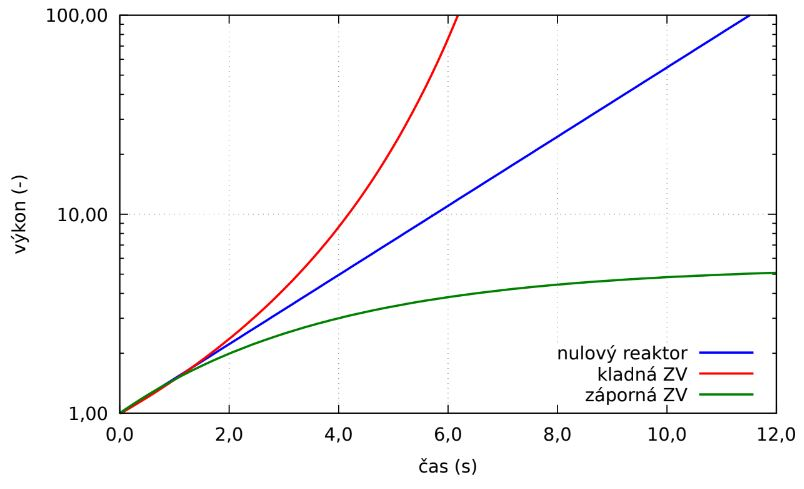
\includegraphics[width=0.7\textwidth]{img/ZV.JPG}
  \caption{Vliv ZV na zavedení kladné reaktivity.}
  \label{ZV}
\end{figure}

Graf dále ukazuje, že při velmi nízkých výkonech (nulový reaktor) všechny křivky splývají, jelikož se vliv ZV zatím neuplatňuje. Lze tedy říci, že každý reaktor se chová jako nulový a každý reaktor má ZV, pouze závisí, od jakého výkonu se začnou projevovat.

Dále je možné ZV rozlišit pomocí fyzikálních vlastností:

\begin{itemize}
  \item jaderné -- změnou teploty se mění mikroskopické účinné průřezy (Doppler), zároveň se může změnit Maxwell-Boltzmannovo rozdělení hustoty toku (maximum se posune do vyšších energií), což má za následek změnu reakčních rychlostí,
  \item hustotní -- změnou teploty se mění hustota jader a tím makroskopické účinné průřezy, nebo geometrické změny ovlivní Buckling.
\end{itemize}

\subsubsection{Doppler}

Dopplerovo rozšíření je kapitola sama o sobě. To se uplatňuje pouze v rezonancích, kde vlivem teplotní změny dochází k poklesu maxima a nárůstu šířky peaku tak, aby plocha pod peakem zůstala konstantní (vlivem teplotní změny atomy více kmitají, a proto se jakoby "rozmazávají"). Jelikož neutron ztrácí svoji energii po skocích, ne kontinuálně, při rozšíření základny rezonance vzniká "větší prostor", kam může neutron spadnout a dojít k záchytu.

Ve výsledku, Dopplerovo rozšíření vždy způsobuje zvyšování abrosbce, otázka je, jestli jde o radiační záchyt, nebo štěpení. Pro okolní materiály mimo palivo (moderátor, chladivo, konstrukce) vždy dochází k radiačnímu záchytu, jde tedy o zápornou ZV která vede k poklesu reaktivity.

U paliva záleží na konkrétním izotopickém složení a obohacení. Například pro U-238 je Doppler velmi významný, jelikož při zpomalování neutronu už ho neutron nemůže štěpit a dochází právě k radičnímu záchytu. Naopak u U-235 by sice došlo k nárůstu absorbce, ale tím i nárůstu štěpení. Je proto důležitý poměr obohacení. Na KIDu jsme si říkali, že při obohacení pod 35\% dojde vždy k převládnutí parazitní abrosrbce na U-238 a tedy k poklesu reaktivity. Pod touto hranicí jde tedy o zápornou ZV (tepelné reaktory), nad tuto hranici je třeba být opatrný, jelikož může vést ke kladné ZV (rychlé reaktory).

\subsubsection{Vodo-uranový poměr}

Tepelné jaderné reaktory potřebují k udržení štěpné řetězové reakce tepelné neutrony, které vznikají zpomalováním v moderátoru. Při změně teploty moderátoru dochází rovněž ke změně jeho hustoty a tím i ke změně makroskopických průřezů a reakčních rychlostí. Při změně teploty moderátoru tak nutně dochází ke změně moderačních vlastností a tím i ke změně reaktivity.

Aby bylo možné analyzovat, jak se změna hustoty moderátoru projeví na změně reaktivity, je třeba určit průběh závislosti reaktivity na hustotě moderátoru (\textbf{vodo-uranový poměr}), viz obrázek \ref{voda-uran}. Z toho lze rozlišit 2 typy moderátoru:

\begin{itemize}
  \item ideální moderátor (modrý) -- moderátor, na kterém nedochází k žádné parazitní absorbci,
  \item skutečný moderátor (červená).
\end{itemize}

\begin{figure}[H]
  \centering
  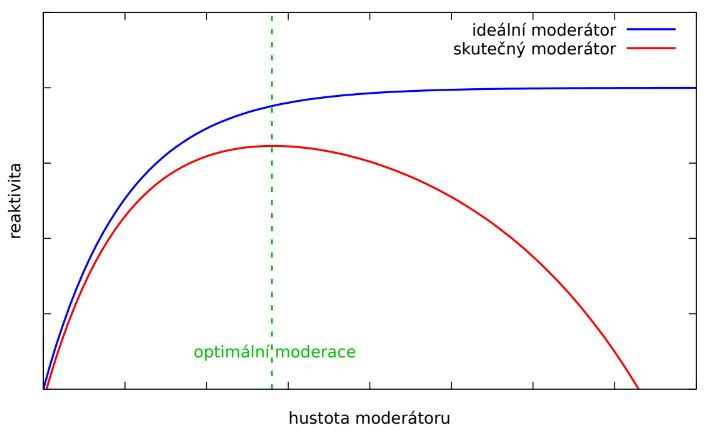
\includegraphics[width=0.7\textwidth]{img/voda-uran.JPG}
  \caption{Závislost reaktivity na hustotě moderátoru.}
  \label{voda-uran}
\end{figure}

Při přidávání ideálního moderátoru dochází pouze k větší termalizaci a žádné parazitní absorbci, proto reaktivita roste a ustaluje se na saturované hodnotě. Ve skutečnosti ale při přidávání moderátoru od jistého okamžiku dojde k převládnutí parazitní absorbce a reaktivita opět klesá. K maximu reaktivity pak dochází při tzv. \textbf{optimální moderaci}, část vlevo se poté nazývá \textbf{podmoderovaná} (méně moderátoru než je optimum) a část vpravo \textbf{přemoderovaná}. Tvar této křivky závisí na konkrétním moderátoru (zde je vidět např. výhoda těžké vody oproti lehké vodě, kdy na těžké dochází k absorbci výrazně méně).

Známe-li tyto grafy, je možné analyzovat, co se stane při změně teploty. Při zvyšování teploty dojde k poklesu hustoty moderátoru, což v řeči grafu \ref{voda-uran} znamená posun doleva. Pokud se budeme nacházet v podmoderované oblasti, dojde k poklesu reaktivity (ZV). Nicméně v přemoderované oblasti dojde k nárůstu (kladná ZV). Z hlediska bezpečnosti je proto důležité mít reaktor v podmoderované oblasti, což je možné ovlivnit: geometrií, obohacením, vyhořením, koncentrací boru apod. Zároveň může docházet k lokálnímu přemoderování (výzkumné reaktory), důležité je ale celkový charakter.

\subsubsection{Dutinový efekt}

V případě varných reaktorů může dojít k varu vody, čímž vnikne prostor s velkým objemem páry (tzv. dutina), což má za následek pokles moderace, ale zároveň opkles absorbce. Otázkou opět je, který efekt převládne.

Pro lehkovodní PWR reaktory platí, že mají záporný dutinový koeficient. Pokud zvýším průtok, zlepší se přenos tepla, dutiny se zmenší a výkonnaroste. To samé zvýší-li se tlak, tak se zvýší bod varu, dutiny se opět zmenší a výkon naroste. To je dobrý bezpečnostní efekt, při LOCE dojde ke snížení tlaku (klesá výkon) a ke snížení průtoku (klesá výkon).

Naopak RBMK má kladný dutinový koeficient, jelikož tam voda není zároveň moderátor. Lepší nestavět.

Pro PWR reaktory jde o nevýznamný efekt, tady dutiny nevznikají. Pokud ano, tak je něco špatně.

\subsection{Zpětnovazební koeficienty reaktivity}

\textbf{Zpětnovazební koeficienty} mohou být jakékoliv (teplotní, hustotní, výkonové), nicméně většinou je stejně vše ovlivněno právě teplotou (teplota ovlivní hustotu, změna výkonu ovlivní teplotu apod.), tudíž se dále zaměříme pouze na ty teplotní. Ty je možné určit dle vztahu:

\begin{equation}
  \boxed{
  a_i = \dfrac{\partial \rho}{\partial T_i}
  \label{zpetnovazebni_koeficient_definice}
  }
\end{equation}

A celkový vliv na reaktivitu jako:

\begin{equation}
  \boxed{
  \rho_{tot} = \sum_i \dfrac{1}{V_i} \int_{V_i} a_i(\bar{r}) \Delta T_i(\bar{r}) \Omega_i(\bar{r}) d\bar{r},
  \label{zpetnovazebni_koeficient_reaktivita}
  }
\end{equation}

kde:

\begin{itemize}
  \item $\Delta T_i$ -- představuje teplotní odchylku od i-té složky (teplotní rozdíl od kritického a aktuálního stavu),
  \item $\Omega_i$ představuje tzv. \textbf{normovanou váhovou funkci}, která opravuje fakt, že stejné teplotní změny mohou mít v jiných místech jiný vliv na reaktivitu. Skutečně jsou úměrné $\Phi^2$.
\end{itemize}

Při použití jednobodové kinetiky je možné zanedbat prostorovou závislost. Pokud se navíc zavede lineární model zpětné vazby, kdy budou koeficienty konstantní (normálně jsou závislé na teplotě), tak se výpočet zjednodušší:

\begin{equation}
  \boxed{
  \rho_{tot} = \sum_i a_i \Delta T_i (t).
  \label{zpetnovazebni_koeficient_reaktivita_1B}
  }
\end{equation}

\subsection{Přenosová funkce zpětné vazby}

Vliv zpětně vazby je možné vyjádřit i pomocí jednobodové kinetiky/dynamiky. Z linearizovaného modelu nulového reaktoru vyplývá (směr "doprava", tedy jak změna reaktivity vede na změnu četnosti):

$$ \dfrac{\Delta \tilde{N}(s)}{N_0} = \tilde{G_0}(s) \cdot \tilde{\rho}(s) = \tilde{G_0}(s) \cdot [ \tilde{\rho_\text{ex}}(s) + \tilde{\rho_\text{ZV}}(s) ], $$

kde $\tilde{\rho_\text{ex}}(s)$ značí vnesenou reaktivitu a $\tilde{\rho_\text{ZV}}(s)$ reaktivitu zpětné vazby. Zároveň je ale tato ZV reaktivita ovlivněna změnou četnosti, proto musí mít vlastní \textbf{přenosovou funkci zpětné vazby} $\tilde{W_\text{ZV}}(s)$, pro kterou platí\footnote{Tentokrát se přenosová funkce ZV definuje "obráceně", viz linearizovaný model v předešlé otázce. Tudíž pro $G_0$ platí, že změna reaktivity ovlivní četnost, ale tady platí, že změna četnosti ovlivní velikost ZV reaktivity.} (směr "doleva", tedy jak změna četnosti ovlivní reaktivitu, nicméně tentokrát pouze tu zpětnovazební):

$$ \tilde{\rho_\text{ZV}}(s) = \tilde{W_\text{ZV}}(s) \cdot \dfrac{\Delta \tilde{N}(s)}{N_0}. $$

Když se to všechno poskládá do sebe, tak je možné získat finální tvar spolu s tzv. \textbf{přenosovou funkcí reaktoru}\footnote{Tentokrát už nenulového.} $\tilde{G}(s)$ ve tvaru:

\begin{equation}
  \boxed{
    \dfrac{\Delta \tilde{N}(s)}{N_0} = \tilde{G}(s) \cdot \tilde{\rho}(s) = \dfrac{\tilde{G_0}(s)}{1 - \tilde{G_0}(s) \tilde{W_\text{ZV}}(s)} \cdot \tilde{\rho}(s).
  }
\end{equation}

Zbývá určit pouze tvar přenosové funkce zpětné vazby, čímž se získá tvar celkové přenosové funkce a vše se může řešit stejnými postupy, jako v případě kinetiky.

Zároveň se ještě hodí znát podmínku stability reaktoru, tedy situaci, jestli se výkon po nějaké době ustálí, nebo diferguje do nekonečna. Zde platí jednoduchý vztah:

\begin{equation}
  \boxed{
    \int_0^\infty  |G(t)| dt < \infty.
  }
\end{equation}

Zde platí, že nulový reaktor je vždy nestabilní. Stabilizuje se pouze až se zápornými ZV.

\subsection{Modely dynamiky reaktoru}

Analytické vyjádření zpětnovazební přenosové funkce je obtížné, často se musí něco zanedbat apod. Existuje několik modelů v závislosti na tom, co se mění (ve všech případech jde o linearizované modely):

\begin{itemize}
  \item Dvousložkový model -- mění se pouze teplota paliva a chladiva (tlakovodní a sodíkové reaktory):\\
  $$ \tilde{W_\text{ZV}}(s) = \dfrac{a_\text{fuel} (1 + s \: \tau_\text{cool}) + a_\text{cool} \: \Gamma}{k_\text{fuel} \: [(1 + s \: \tau_\text{cool})(1 + s \: \tau_\text{fuel}) - \Gamma]} $$
  \item Jednosložkový model -- pouze jedna teplota (molten salt):\\
  $$ \tilde{W_\text{ZV}}(s) = \dfrac{a_\text{power}}{1 + s \: \tau}. $$
  \item Adiabatický model -- rychlé změny, kdy se teplo nestačí odvézt:\\
  $$ \tilde{W_\text{ZV}}(s) = \dfrac{a_\text{fuel}}{s \: C_\text{fuel}}. $$
\end{itemize}

Ve všech případech: $a$ značí koeficient reaktivity, $C$ tepelnou kapacitu, $k$ součinitel prostupu tepla a konstanty $\tau$ a $\Gamma$ jsou jisté časové, resp. bezrozměrné konstanty, které pouze zjednodušují zápis a pro každý model se volí jinak. Více modelů a jejich odvození je v Bédových skriptech.


\section[Monte-Carlo]{Princip metody Monte Carlo, analogová a neanalogová metoda, srovnání s deterministickými metodami}

\subsection{Základní filosofie}

Základním principem pro deterministické kódy je přímé řešení matematických rovnic popisujících chování v jaderném reaktoru, tedy difúzní rovnice, nebo transportní rovnice. Máme tedy jasný matematický model a ten řešeíme pomocí numeriky.

Oproti tomu stochastické metody ke svému řešení žádné rovnice nepotřebují a simulují přímo konkrétní částice. Modelování tedy probíhá na takovém prinicpu, že se jasně stanoví geometrie a pomocí generátoru náhodných čísel se generují imaginární částice, které s danými geometriemi interagují. To, jak budou částice interagovat čistě závisí na účinných průřezech (je potřeba znát diferenciální průřezy, jelikož nás i zajímá směr příletu/odletu částice). 

Z této základní filosofie tedy platí jasné rozdíly mezi deterministickými a stochastickými metodami:

Deterministické:
\begin{itemize}
  \item Rychlejší, ale přesné pouze tak, jak přesný je daný matematický model.
  \item Získám jeden výsledek bez nejistot (ačkoliv nejistoty jsou dané zjednodušeními, není je tak jednoduché vyčíslit).
  \item Složité modelování geometrie $\rightarrow$ aplikují se různá geometrická zjednodušení (nekonečná mříž, 2D aproximace apod.)
  \item Účinné průřezy se musejí grupovat $\rightarrow$ je potřeba více programů a více přístupů (nejprve příprava v rámci jednoho souboru pomocí transportky, poté aplikace ve velkém celozónovém modelu pomocí difúzní rovnice).
\end{itemize}

Stochastické:
\begin{itemize}
  \item Pomalejší, ale teoreticky přesnější. S rozvojem techniky se dá očekávat převládnutí. Přesnost je ovlivněna hlavně účinnými průřezy, a pak trochu generací pseudonáhodných čísel.
  \item Vždy mi nástroj vyplivne výsledek s danou nejistotou, kterou je teoreticky možné snížit simulací většího počtu částic.
  \item Jednoduché 3D modelování.
  \item Spojité účinné průřezy (lze získat pomocí NJOY).
\end{itemize}

Stochatické metody tedy nepotřebují žádné matematické rovnice, celý výpočet probíhá pomocí tzv. \textbf{náhodné procházky} metodou Monte-Carlo, což je dále rozebráno v další otázce.

Jako částice je možné simulovat absolutně cokoliv, záleží na znalosti účinných průřezů a rozšíření výpočetního kódu:
\begin{itemize}
  \item Serpent 2 -- hlavní využití pro reaktorovou fyziku, specializuje se tedy převážně na neutrony (ačkoliv by měl nějak zohledňovat i (n,$\gamma$) reakce, ze zkušenosti se mi zdá, že to moc nefunguje).
  \item MCNP 6 -- momentálně asi nejznámnější kód, umí modelovat neutrony, fotony, elektrony..., skoro cokoliv. Bere se jako benchmark pro ostatní kódy, ale je složitý na syntaxi a zdlouhavý.
  \item OpenMC -- o tom moc nevím. Dobrý je, že je zadarmo.
  \item KENO -- low-budget alternativa od Scaleu. Prý stojí za prd, ale umí hezky spolupracovat s ostatními SCALE balíky, tudíž se taky může hodit.
\end{itemize}

\subsection{Analogová a neanalogová metoda}

Základním principem \textbf{analogové metody} je to, že trekujeme konkrétní neutrony, které když zaniknou (absorbcí či únikem), tak prostě zaniknou a dál neexistují. Při výpočtu skórování v datém detektoru/tallies se tedy započítávají s váhou 1. Tato metoda více odpovídá realitě, nicméně je zdlouhavá, jelikož pro přesnější výsledek je nutné simulovat větší populaci částic.

To platí např. pro prostředí s velkou absorbcí a malým zdrojem (chceme-li např. řešit problematiku stínění, reflektoru apod.)

Oproti tomu \textbf{neanalogová metoda} či \textbf{implicitní metoda} funguje tak, že narodí-li se částice, tak je jí přiřazena váha 1. A tím, jak se částice toulá po daném systému, tak interaguje s prostředím až do místa, kde by teoreticky mělo dojít k její absorbci. Nicméně, nedojde k úplné absorbci, pouze se dojde k započítání do skórování a dále se jí srazí váha na nižší hodnotu. Nedojde tedy k zániku, a jedna částice může pokračovat v toulání se po systému. Pouze má nižší váhu, proto narazí-li na další absorbci, opět dojde k započtení do skórování, ale s nižší váhou, jelikož v tomto druhém místě by už částice neměla teoreticky existovat. Dojde-li po několika srážkách ke snížení váhy pod jistou hladinu, až tehdy dojde k celkovému zániku dané částice.

Tímto způsobem se dají zpřesnit výsledky za pomoci menšího počtu částic. Nicméně, jde o komplikovanější metodu a je potřeba znát širší matematický základ. V prvním případě je důležité určit, jakým zpsůobem se změní váha dané částice. Tato technika se nazývá \textbf{redukce variance} (redukce variance, jelikož zpřesňují výsledek a snižuji rozptyl, tedy varianci).

\subsection{Redukce variance}

První možností při sražení váhy je za pomoci teoretické absorbce. To se určí jednoduše dle vztahu:

$$ w = w' \left ( 1-\dfrac{\Sigma_\text{a}}{\Sigma_\text{t}} \right ). $$

Dále je třeba určit, při jaké energii dojde ke skutečnému zániku částice, jelikož trekování částice s příliš malou váhou je naopak kontraproduktivní. To se určuje dle tzv. Ruské rulety, jejíž nejjednodušší zápis je ve tvaru:

$$ P = 1-\dfrac{w}{w_0}, $$

kde $w_0$ značí váhu na začátku historie a $P$ značí pravděpodobnost, při které dojde k zániku.

Dále je možné podobnou metodu aplikovat na vznik částic (z hlediska neutronů štěpení (n,xn) reakce). V takovém případě se nová váha určí jako:

$$ w = w' \nu. $$

Tohle jsou jenom základní metody, ve skutečnosti je nutné aplikovat více metod redukce variance. Těmi hlavními jsou:

\begin{itemize}
  \item cut-off -- zánik při poklesu pod jistou hladinu (energetické, váhové, časové apod.),
  \item splitting -- rozdělení na 2 částice, každá s jinou váhou (geometrické, energetické, časové),
  \item ruská ruleta -- naopak zánik dané částice, kombinace se splittingem (velká váha splitting, malá váha ruská ruleta),
  \item biassing -- to je to zmiňované sražení váhy (absorbcí).
\end{itemize}

Nicméně nejdůležitější je pochopitelně kombinace všeho.

\section[Náhodná procházka]{Náhodná procházka při simulaci životního cyklu neutronů v jaderném reaktoru}

Jak bylo zmíněno, ýpočty ve stochatických kódech probhají díky simulaci tzv. \textbf{random walks - náhodné procházky} dané částice, tedy simulace skutečného života dané částice. K tomu je potřeba znát pár základů.

\subsection{Matematická vsuvka}

\subsubsection{Generace pseudonáhodných čísel}

Jde o stochastickou/pravděpodobnostní metodu, tedy základem je generování náhodných čísel. Jelikož ke generaci dochází strojově, nebude nikdy možné stanovit skutečně náhodná čísla, pouze tzv. pseudonáhodná. O to větší problém je vytvořit sekvenci náhodných/pseudonáhodných čísel tak, aby se neopakovaly. K tomu se ve většině kódů využívá tzv. \textbf{linear congruential random numbers generator}:

$$ S_{i+1} = ( S_i \cdot g + c ) \: \text{mod} \: 2^m, $$

kde $S_i$ značí seed (typicky nějaké velké číslo, pokaždé jiné), $g$ značí generátor/násobič (opět veliké číslo, to může být stejné), $c$ značí přírůstek (může být 0, 1, nebo opět jakékoliv) a z toho všeho určíme modulus (tedy zbytek po dělení) nějakého čísla $2^m$.

Přesnou kombinací těchto čísel je možné stanovit konkrétní generátor, např. MCNP využívá: $m = 63$, $g$ je různé a $c = 1$.

\subsubsection{Random Sampling - Náhodné vzorkování}

Dále je potřeba navzorkovat daná čísla podle jistých pravděpodobnostních funkcí $f(x)$. Generátor náhodných čísel nám poskytne uniformní rozdělení na intervalu (0,1), nicméně např. k rozptylu dochází pod jistým úhlem s danou pravděpodobností, nebo energie vzniklých neutronů také mají jistou pravděpodobnost.

Máme-li tedy danou pravděpodobnostní funkci (PDF) $f(x)$ normovanou na 1. Z té jsme schopni určit distribuční funkci (CDF) $F(x)$ jako postupný integrál:

$$ F(x) = \int_{-\infty}^x f(y) \text{d}y. $$

Označíme-li uniformní náhodná čísla jako $\xi$, ale my chceme získat/navzorkovat hodnoty $x$, pak tedy hledáme relaci mezi:

$$ F(x) = \xi \iff x = F^{-1}(\xi). $$

To je možné určit:

\begin{itemize}
  \item \textbf{direct sampling - přímé vzorkování}, tedy napřímo. Není možné vždy, může být zdlouhavé a koplikované (jednoduché např. u konstanty).
  \item \textbf{rejection sampling - metoda odmítnutí}, mnohem více univerzálmí metoda.
\end{itemize}

Nejprve se stanoví konstanta $c \geq 1$ a další hraniční PDE $g(x)$ kterou je možné navzorkovat napřímo (např. konstanta) tak, aby pro všechna $x$ platilo:

$$ f(x) \leq c g(x). $$

Nejprve navzorkuji danou $\bar{x}$ z funkce $g(x)$ (to je jednoduché, udělám to napřímo). Dále naleznu nějakou hodnotu $\xi$  jednotkového intervalu (0,1), a pokud platí, že:

$$ \xi \leq \dfrac{f(\bar{x})}{c g(\bar{x})}, $$

pak mohu s jistotou říci, že zároveň $\bar{x}$ je navzorkována i z původní $f(x)$. Je to v podstatě stejný způsob, jako když se integrauje přes Monte-Carlo. Vybírám hodnoty z intervalu (0,$cg(x)$), a pokud platí, že hodnota je zároveň v intervalu (0,$f(x)$), tak ji vezmu, jinak ne, viz obrázek \ref{rejection}.

\begin{figure}[H]
  \centering
  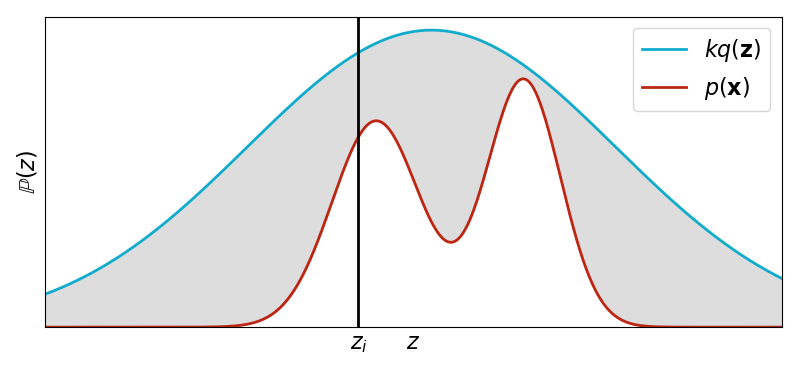
\includegraphics[width=0.7\textwidth]{img/rejection_sampling.png}
  \caption{Metoda odmítnutí.}
  \label{rejection}
\end{figure}

\subsection{Popis náhodné procházky}

Schematicky je náhodná procházka jednoduchá:

\begin{enumerate}
  \item[1.] Vznik -- částice nejprve vznikne, buď z externího zdroje, nebo za pomoci štěpení či (n,xn) reakce.
  \item[2.] Tracking -- částice se nějak pohybuje v daném prostředí. Sleduje se kudy prochází, jakými geometrickými hranicemi apod.
  \item[3.] Reakce -- tím, jak částice prochází prostředím, tak interaguje s okolní látkou, čímž se mění její směr, energie a v případě implicitní metody i váha
  \item[4.] Detektory/Tallies -- statistické vyhodnocení dané reakce.
  \item[5.] Zánik -- případné vyhodnocení za pomoci redukce variance.
\end{enumerate}

Toto se opakuje tisíckrát-milionkrát. 4ím větší geometrie, tím více částic je potřeba na detailnější prozkoumání celého systému. Na základě všech dat se poté vyhodnotí detektory, koeficient násobení, reakční rychlosti apod.

\subsubsection{Vznik}

Částice nejprve vznikne. Pokud máme externí zdroj, tak je dopředu nadefinováno energetické a směrové rozdělení. Pokud jde o zdroj ze štěpení, tak je třeba uvažovat energetické vzorkování přes štěpné spektrum a uniformní směrovou distribuci.

\subsubsection{Tracking}

Pokud znám počáteční energii a směr, je třeba určit, za jakou dobu dojde k další reakci (která se bude odehrávat na jiném místě). Opět se postupuje přes pravděpodobnostní PDE funkci ve tvaru:

$$ f(x) = \Sigma_\text{t} e^{-x \Sigma_\text{t}} $$

a distribuční CDF funkci:

$$ F(x) = 1 - e^{-x \Sigma_\text{t}}. $$

V tomto případě je CDF funkci možné vyjádřit pomocí přímého vzorkování jako:

$$ x = -\dfrac{1}{\Sigma_{\text{t}}} \text{ln}(1-\xi) = -\dfrac{1}{\Sigma_{\text{t}}} \text{ln}(\xi), $$

kde $\xi = F(x)$ navzorkujeme rovnoměrně z intervalu (0,1). 

Tohle platí, je-li geometrie složena homogenně pouze z jednoho materiálu. Máme-li ale geometrii s různými materiály (a tedy i různými $\Sigma_{t})$, je třeba postupovat postupně. Rozlišují se 2 přístupy:

\begin{itemize}
  \item Surface-tracking,
  \item Delta-tracking.
\end{itemize}

V případě \textbf{Surface-trackingu} se uplatňují izolované 2 výpočty před a za hranicí (tedy v materiálu 1 a 2). Má-li být zvdálenost mezi reakcemi $x$ delší, než je přímá trasa k hranici $d$ (tedy dojde-li k překročení hranice), musí se výpočet rozepsat, protože v novém materiálu už zbylé $x$ bude logicky jiné, kvůli jinému $\Sigma_\text{t}$. V novém materiálu tedy platí:

$$ e^{-x_2 \Sigma_2} = e^{-(x_1-d)\Sigma_2} $$

z čehož se vyjádří $x_2$ a pro celou dráhu $x$ bude platit:

$$ x = d + x_2 = d + (x_1 - d) \dfrac{\Sigma_1}{\Sigma_2}. $$

Opět, platí-li, že $x_2$ je opět větší než vzdálenost k další hranici, postupujeme pořád obdobně, dokud nevyjde, že $x_i$ skutečně skončí v daném materiálu. Hlavní filosofie tedy je, že se výpočet na každé hranici zastaví a podle aktuálního $\Sigma_\text{t}$ se přepočte vzdálenost mezi reakcemi $x$.

V případě \textbf{Delta-trackingu} se postupuje jinak, bez zastavování se na každé hranici. Cílem je stanovení virtuálního $\Sigma_0$, který by reprezentoval veškeré materiály nacházející se v daném směru, dle vztahu:

$$ \Sigma_0 = \Sigma_\text{m} - \Sigma_\text{t}, $$

kde $\Sigma_\text{m}$ značí maximální možný průřez, který se v systému vyskytuje (dává tedy horní odhad). Známe-li počáteční směr, určí se vzdálenost $x$ mezi reakcemi za pomocí pouze $\Sigma_\text{m}$ (tím získáme dolní odhad vzdálenosti), kde dojde k virtuální reakci. To, jestli dojde či nedojde k reakci, se určí dle pravděpodobnosti:

$$ P = \dfrac{\Sigma_0}{\Sigma_\text{m}} = 1 - \dfrac{\Sigma_\text{t}}{\Sigma_\text{m}}. $$

Pokud dojde k zamítnutí, proces pokračuje dál, dokud nedojde ke skutečné reakci. Výhody Delta-trackingu jsou patrné hlavně v momentu, kdy geometrie obsahuje spoustu ploch.

\subsubsection{Reakce}

Nyní jsme už v bodě, kde dojde k nějaké reakci, zbývá zjistit k jaké. To se opět určí pravděpodobnostně, tedy to, že dojde k $i$-reakci na $m$-izotopu určuje vztah:

$$ P = \dfrac{\Sigma_{i,m}}{\Sigma_\text{t}}. $$

V případě absorbce se dále může uplatnit redukce variance. V případě rozptylu se dále musí určit, pod jakým úhlem a s jakou energií se neutron rozptýlí. V případě štěpení kolik neutronů se emituje, atd. 

\subsubsection{Detektory}

V posledním případě zbývá zaznamenat dané reakce a určit nějakou integrální hodnotu. Může jít o hustotu toku, hustotu proudu, reakční rychlosti apod. Dá se postupovat analogově/implicitně, viz předešlá otázka.

Neméně důležité je zapracování nejistot. U výsledků se předpokládá Gaussovské rozdělení kolem nějaké střední hodnoty s daným rozptylem. Čím větší statistika, tím menší rozptyl. K tomuto určování se aplikují jakési matematicko-statistické nástroje, o kterých nemám ponětí, nicméně bavili jsme se o tzv. \textbf{Central Limit Theorem}, který tohleto umí dělat.

Výsledky jdou posléze i kombinovat mezi sebou. Dále se hodí vědět, že celkový rozptyl klesá s odmocninou celkové generace, tedy:

$$ \sigma^2 = \dfrac{\sigma^2_i}{N}. $$

\subsubsection{Zánik}

Nakonec neutron zanikne a už dále neexistuje :(
\section[Vyhořívání]{Výpočty vyhoření jaderného paliva, formulace úlohy a metoda prediktor-korektor}

UPRAVIT!!

\subsection{Výpočty vyhoření}

Vyhoření se počítá pomocí Batemanových rovnic:

\begin{equation}
  \dfrac{\text{d}n_i}{\text{d}t} = -\sigma_i \phi n_i + \sum_{j \to i} \gamma_i \sigma_j \phi n_j - \lambda_i n_i + \sum_{j \to i} \gamma_i \lambda_j n_j,
\end{equation}

nicméně aby šly dopočíst, je třeba znát hodnotu $\phi$, která se časem mění. Proto se postupuje pomocí tzv. metody \textbf{prediktor-korektor}, která nejprve odhadne $\phi$ na začátku cyklu, dopočte na konec cyklu (prediktor), přepočte novou $\phi$ z konce. Z těchto dvou hodnot poté stanoví průměr (korektor) a dopočte nové složení na konci cyklu.

Proto je důležité vhodně stanovit délku kroku. Například u tepelných systémů je třeba počáteční kroky volit velmi krátké, jelikož dochází k ustalování koncentrace xenonu, což má za následek velký nárůst $\phi$. U rychlých systémů to tak kritické není.

Nicméně, tato metoda je pouze na odhad hustoty toku. Stále máme kombinaci LDR o hodně členech (např. ENDF/B-VIII.0 1600 nuklidů). Vypíšu 2 metody řešení:

\subsubsection{MATREX metoda}

Maticovou formu Batemanových rovnic:

\begin{equation}
  \dfrac{\text{d}\vec{N}}{\text{d}t} = \textbf{A} \vec{N}(t)
\end{equation}

řeším ve formě exponenciály:

\begin{equation}
  \vec{N}(t) = \text{exp} (\textbf{A}t) \vec{N}(0),
\end{equation}

$$ \text{exp} (\textbf{A}t) = \sum_{k=0}^\infty \dfrac{(\textbf{A}t)^k}{k!}. $$

\subsubsection{CRAM metoda}

Neboli aproximace pomocí Chebyshevových racionálních funkcí. Obyčejně se využívá CRAM metoda 16. řádu, která má stejnou přesnost, jenom je rychlejší než MATREX metoda.

Funguje na stejném základu, pouze rozkládá exponenciální matici do Chebyshevových racionálních funkcí:

$$ \vec{N}(t) = \left [ \sum_{k=0}^\infty \dfrac{(\textbf{A}t)^k}{k!} \right ] \vec{N}(0) \approx \left [ \alpha_{0,K} \textbf{I} + 2 \text{Re} \left [ \sum_{j=1}^{K/2} \left ( -\dfrac{\alpha_{j,K}}{\theta_{j,K}} \right ) \left ( \textbf{I} + \textbf{A} \left ( -\dfrac{t}{\theta_{j,K}} \right ) \right ) ^{-1} \right ] \right ] \vec{N}(0), $$

kde $K$ představuje řád a $\alpha_{i,j}$ a $\theta_{i,j}$ jsou příslušné CRAMerovy koeficienty k dohledání v literatuře.
\section[Celozónové výpočty]{Celozónové výpočty jaderných reaktorů, příprava makroskopických dat pro celozónové výpočty a používané předpoklady}

UPRAIT!

\subsection{Transportní (deterministický) výpočet}

Ve zkratce: 

\begin{enumerate}
  \item[1.] Nejprve si vymyslím, jakou knihovnu dat použiji a pro tu šáhnu (např. \textbf{ENDF/B}. Jde o bodové knihovny a každá má různý počet bodů pro různé materiály).
  \item[2.] Tato nezpracovaná data je potřeba zpracovat (zgrupovat, upravit na teplotu apod.) vhodným nástrojem (např. \textbf{NJOY}), čímž vzniká pracovní knihovna obsahující stovky až tisíce grup.
  \item[3.] Následuje \textbf{Lattice výpočet} pomocí nějakého mikrokódu (např. \textbf{Newt/TRITON}, \textbf{Helios}), často v nekonečné mříži (pro tepelné systémy to stačí) pomocí transportní teorie. Tento model už by měl zohledňovat samostínění. Homogenizovat je možné i stochasticky bez aplikace transportní teorie (např. \textbf{Serpent}).
  \item[4.] Tím dochází k homogenizaci a k tvorbě homogenizovaných dat (difúzní koeficient, makroskopické průřezy apod.) pro daný palivový soubor. Zároveň se slučují grupy do menšího počtu (tepelný systém stačí 2, rychlé 4, lépe 8, záleží na složení. Neplechu dělá větší množství Pu, kde je potřeba více grup).
  \item[5.] Homogenizované veličiny putují do celozónového výpočtu makrokódem (např. \textbf{PARCS}, \textbf{Andrea}), který častou pouze s pomocí difúzního přiblížení určí hledané parametry (kritičnost, energetická distribuce, vyhoření apod.).
\end{enumerate}

\subsubsection{Homogenizace}

Pro deterministické kódy se postupuje podobně, jako při grupování mikroskopických průřezů, akorát že teď se grupují makroskopické průřezy vážené hustotou toku a nově i objemem. Opět se musí zachovat reakční rychlost:

\begin{equation}
  \boxed{
    \Sigma_G = \dfrac{\sum_{h \in G} \sum_i V_i \Sigma_{i,h} \Phi_{i,h}}{\sum_{h \in G} \sum_i V_i \Phi_{i,h}}.}
\end{equation}

Problém je, že takto homogenizovaná data jde použít pouze na původně řešený problém, nepaltí tedy obecně. Při změně geometrie se musí homogenizovat znovu. Pro následující nodální výpočet nám jde o:

\begin{itemize}
  \item $\Sigma_\text{tr}$ -- převrácená hodnota představuje dráhu, kterou neutron urazí po nekonečném množství srážek. Potřebujeme znát pro výpočet difúzního koeficientu, který se používá v difúzním přiblížení. Pro jeho určení se vychází z In-scatter nebo Out-scatter aproximace (nebo obojího), což je rozdíl totálního průřezu a sumy rozptylových průřezů z rychlé grupy.
  \item $\Sigma_\text{a}$ -- představuje zánik neutronů.
  \item $\nu \Sigma_\text{f}$ -- představuje produkci neutronů.
  \item $\kappa \Sigma_\text{f}$ -- představuje energii ze štěpení.
  \item $\Sigma_\text{s, g - g'}$ -- vyjadřuje přechod mezi grupami. 
  \item relativní výkony jednotlivých proutků.
\end{itemize}

Pro zachování spojitosti hustoty proudu mezi soubory se využívají tzv. ADF (Assembly Discontinuity Factors).

Homogenizace ve štěpném prostředí (speciálně pro tepelné reaktory, rychlé si myslím že jsou obtížnější) probíhá v nekonečné mříži za použití zrcadlových hraničních podmínek. To má v sobě některá úskalí:

\begin{itemize}
  \item Neuvažuje se únik, který tam ve skutečnosti je. Ten je možné opravit pomocí B1 aproximace, což je oprava přes hranice souboru na základě kritičnosti. Jednoduše řečeno, k totální grupové reakční rychlosti se přičte/odečte B-násobek grupové hustoty proudu tak, aby došlo k dosažení kritického stavu, čímž se získají zbylé homogenizované průřezy.
  \item Neuvažuje se prostorový gradient hustoty toku (v celozónovém výpočtu není hustota toku ve všech souborech středově souměrná). Oprava pomocí rehomogenizace, která kombinuje hustotu toku v nekonečné mříži a hustotu toku z celozónového výpočtu, která se získala po dosazení původních dat. Je důležité hlavně v blízkosti silných absorbátorů, kde je gradient hustoty toku významný.
  \item Spektrum (teď nemyslím prostorové, ale energetické) neodpovídá skutečnosti.
\end{itemize}

Homogenizace v neštěpném prostředí je obtížnější, protože tady už tuplem neznáme spektrum neutronů. Jsou zde jiné hraniční podmínky (vacuum v okolí reflektoru, reflective/periodic v okolí souborů), nepoužívá se B1 aproximace. Pro anizotropní rozptyl na vodíku se zavádí speciální opravná funkce, která se dá získat výpočtem v 1D prostředí pomocí In-scatter aproximace.

\subsubsection{Parametrizace}

Homogenizace se provádí pro různé stavy řešeného systému, tzv. odskoky. Celozónový výpočet totiž potřebuje data, která jsou závislá na provozu reaktoru (změní-li se teplota paliva, jak se změní homogenizovaná data). Odskoky se provádí např. na teplotě (moderátoru i paliva), vyhoření, hustotě (moderátoru) a koncentraci absorbátoru.

Odskoky fungují tak, že se změní zkoumaný parametr (stačí jednou nahoru a podruhé dolu), systém se zhomogenizuje a výsledná data se proloží lineárním (či jiným) fitem. Tak se získá závislost homogenizované veličiny na měnícím se parametru. Jde to i složitě, mohou se např. měnit 2 parametry najednou (což dle Pavla dává mnohem lepší výsledky), prokládání fitem se může lišit apod.

Mzi odskoky v klasické provozní fyzice patří:

\begin{itemize}
  \item teplota a hustota moderátoru $\dfrac{\partial \Sigma}{\partial T_\text{M}}$,
  \item teplota paliva $\dfrac{\partial \Sigma}{\partial \sqrt{T_\text{P}}}$,
  \item koncentrace kyseliny borité $\dfrac{\partial \Sigma}{\partial C_\text{B}}$,
  \item regulačních tyčí $\alpha$.
\end{itemize}

Takto získám původní provozní sadu průřezů, parametrizované odskoky a pro nové průřezy pak platí:

\begin{equation}
  \boxed{
    \Sigma (T_\text{M}, T_\text{P}, C_\text{B}, \text{CR}) = \Sigma + \dfrac{\partial \Sigma}{\partial T_\text{M}} \Delta T_\text{M} + \dfrac{\partial \Sigma}{\partial \sqrt{T_\text{P}}} \Delta \sqrt{T_\text{P}} + \dfrac{\partial \Sigma}{\partial C_\text{B}} \Delta C_\text{B} + \alpha \Delta \Sigma_\text{CR}.}
\end{equation}

\subsubsection{Celozónový výpočet}

Po takto zhomogenizovaných a zparametrizovaných souborech následuje celozónový výpočet. Ten probíhá buď pomocí zjednodušeného difúzního přístupu, nebo pomocí Simplified P3 metody transportní rovnice (SP3).

Obecně jsou 2 přístupy:

\begin{itemize}
  \item Diferenční přístup -- derivace se nahradí diferencemi a postupuje se pomocí sítí. Je to metodicky snažší, ale zdlouhavé. Objemové elementy jsou mezi sebou vázány přes hustotu toku (rovnost na hranici) a systém vede na soustavu rovnic, která je řešitelná triagonální maticí se 2 neznámými ($\Phi$ a $k_\text{ef}$). Nejprve se provede počáteční odhad a pak se iteruje, dokud se nedokonverguje k nějaké hodnotě $\Phi$ (vnitřní iterace), pomocí které se získá nový $k_\text{ef}$ (podělí se zdroj neutronů z iterace 0 a 1, vnější iterace). Vnější iterace končí po dosažení nějakého kritéria.
  \item Nodální přístup -- hustota toku se rozvine do bazických funkcí, a pak je možné redukovat objemové elementy až na úroveň celého souboru (nódy). Rychlejší, ale fakt složité.
\end{itemize}

Celozónové kódy musí být rychlé a jednoduché. Dále se nabízí coupling s termohydraulickým kódem (RELAP, TRACE), ale to je už fakt hardcore, protože nikdo pořádně neví, jak k tomu přistupovat.
\section[Citlivostní analýza]{Zdroj nejistot numerických výpočtů v jaderných datech a analýza citlivosti koeficientu násobení}

\end{document}
